%% This is file `elsarticle-template-1-num.tex',
%%
%% Copyright 2009 Elsevier Ltd
%%
%% This file is part of the 'Elsarticle Bundle'.
%% ---------------------------------------------
%%
%% It may be distributed under the conditions of the LaTeX Project Public
%% License, either version 1.2 of this license or (at your option) any
%% later version.  The latest version of this license is in
%%    http://www.latex-project.org/lppl.txt
%% and version 1.2 or later is part of all distributions of LaTeX
%% version 1999/12/01 or later.
%%
%% Template article for Elsevier's document class `elsarticle'
%% with numbered style bibliographic references
%%
%% $Id: elsarticle-template-1-num.tex 149 2009-10-08 05:01:15Z rishi $
%% $URL: http://lenova.river-valley.com/svn/elsbst/trunk/elsarticle-template-1-num.tex $
%%
\documentclass[review,12pt]{elsarticle}

%% Use the option review to obtain double line spacing
%% \documentclass[preprint,review,12pt]{elsarticle}

%% Use the options 1p,twocolumn; 3p; 3p,twocolumn; 5p; or 5p,twocolumn
%% for a journal layout:
%% \documentclass[final,1p,times]{elsarticle}
%% \documentclass[final,1p,times,twocolumn]{elsarticle}
%% \documentclass[final,3p,times]{elsarticle}
% \documentclass[final,3p,times,twocolumn]{elsarticle}
%% \documentclass[final,5p,times]{elsarticle}
%% \documentclass[final,5p,times,twocolumn]{elsarticle}

%% The graphicx package provides the includegraphics command.
\usepackage{graphicx}
%% The amssymb package provides various useful mathematical symbols
\usepackage{amssymb}
\usepackage{amsmath}
\usepackage{graphicx}
\usepackage{algorithm}
\usepackage[noend]{algorithmic}
\usepackage{mathtools}
\usepackage{multirow}
\usepackage{url}
\usepackage[normalem]{ulem}
\useunder{\uline}{\ul}{}
\usepackage{subcaption}
%
%% The amsthm package provides extended theorem environments
%% \usepackage{amsthm}

%% The lineno packages adds line numbers. Start line numbering with
%% \begin{linenumbers}, end it with \end{linenumbers}. Or switch it on
%% for the whole article with \linenumbers after \end{frontmatter}.
\usepackage{lineno}


%% natbib.sty is loaded by default. However, natbib options can be
%% provided with \biboptions{...} command. Following options are
%% valid:

%%   round  -  round parentheses are used (default)
%%   square -  square brackets are used   [option]
%%   curly  -  curly braces are used      {option}
%%   angle  -  angle brackets are used    <option>
%%   semicolon  -  multiple citations separated by semi-colon
%%   colon  - same as semicolon, an earlier confusion
%%   comma  -  separated by comma
%%   numbers-  selects numerical citations
%%   super  -  numerical citations as superscripts
%%   sort   -  sorts multiple citations according to order in ref. list
%%   sort&compress   -  like sort, but also compresses numerical citations
%%   compress - compresses without sorting
%%
%% \biboptions{comma,round}

% \biboptions{}

\journal{Applied Soft Computing}

\newcommand{\ASF}{{\sc asf}}
\newcommand{\CMOGA}{{\sc c-moga}}
\newcommand{\MOGA}{{\sc moga}}
\newcommand{\AEPD}{{\sc aepd}}
\newcommand{\NP}{{\sc np}}
\newcommand{\RTS}{{\sc rts}}
\newcommand{\IEEE}{{\sc ieee}}
\newcommand{\CEC}{{\sc cec}}
\newcommand{\COMB}{{\sc comb}}
\newcommand{\PS}{{\sc ps}}
\newcommand{\DE}{{\sc de}}
\newcommand{\DCS}{{\sc dcs}}
\newcommand{\EA}{{\sc ea}}
\newcommand{\EAS}{{\sc ea}s}
\newcommand{\GDEIII}{{\sc gde3}}
\newcommand{\HGSADC}{{\sc hgsadc}}
\newcommand{\MOEA}{{\sc moea}}
\newcommand{\MOEAD}{{\sc moea/d}}
\newcommand{\MOEADDE}{{\sc moea/d-de}}
\newcommand{\MOEAS}{{\sc moea}s}
\newcommand{\MOP}{{\sc mop}}
\newcommand{\MOPS}{{\sc mop}s}
\newcommand{\NSGA}{{\sc nsga}}
\newcommand{\NSGAII}{{\sc nsga-ii}}
\newcommand{\NSGAIII}{{\sc nsga-iii}}
\newcommand{\IBEA}{{\sc ibea}}
\newcommand{\VSDMOEA}{{\sc vsd-moea}}
\newcommand{\VSDMOEAD}{{\sc vsd-moea/d}}
\newcommand{\AVSDMOEAD}{{\sc avsd-moea/d}}
\newcommand{\RMOEA}{{\sc r2-emoa}}
\newcommand{\RR}{{\sc r2}}
\newcommand{\REMOA}{{\sc r2-emoa}}
\newcommand{\WFG}{{\sc wfg}}
\newcommand{\UF}{{\sc uf}}
\newcommand{\DTLZ}{{\sc dtlz}}
\newcommand{\AASF}{{\sc aasf}}
\newcommand{\HV}{{\sc hv}}
\newcommand{\SBX}{{\sc sbx}}
\newcommand{\PF}{{\sc pf}}
\newcommand{\GDEA}{{\sc gdea}}
\newcommand{\KPone}{{\sc kp1}}
\newcommand{\KPtwo}{{\sc kp2}}
\newcommand{\MMEA}{{\sc mmea}}
\newcommand{\CMAES}{{\sc cma-es}}
\newcommand{\DIVA}{{\sc diva}}
\newcommand{\CMOEA}{{\sc c-moea}}
\newcommand{\UD}{{\sc ud}}
\newcommand{\GLP}{{\sc glp}}
\newcommand{\ADI}{{\sc adi}}
\newcommand{\BTS}{{\sc bt}s}
\newcommand{\BT}{{\sc bt}}
\newcommand{\IGD}{{\sc igd}}


\begin{document}

\begin{frontmatter}

%% Title, authors and addresses

\title{Supplementary Document for ``The Importance of Diversity in the Variable \\ Space in the Design of Multi-objective \\Evolutionary Algorithms''}

%% use the tnoteref command within \title for footnotes;
%% use the tnotetext command for the associated footnote;
%% use the fnref command within \author or \address for footnotes;
%% use the fntext command for the associated footnote;
%% use the corref command within \author for corresponding author footnotes;
%% use the cortext command for the associated footnote;
%% use the ead command for the email address,
%% and the form \ead[url] for the home page:
%%
%% \title{Title\tnoteref{label1}}
%% \tnotetext[label1]{}
%% \author{Name\corref{cor1}\fnref{label2}}
%% \ead{email address}
%% \ead[url]{home page}
%% \fntext[label2]{}
%% \cortext[cor1]{}
%% \address{Address\fnref{label3}}
%% \fntext[label3]{}


%% use optional labels to link authors explicitly to addresses:
%% \author[label1,label2]{<author name>}
%% \address[label1]{<address>}
%% \address[label2]{<address>}

\author[label1]{Carlos~Segura}
\ead{carlos.segura@cimat.mx}
\author[label1]{Joel~Chacón~Castillo}
\ead{joel.chacon@cimat.mx}
\author[label2]{Oliver~Sch\"{u}tze}
\ead{shuetze@cs.cinvestav.mx}

\address[label1]{Center for Research in Mathematics (CIMAT), Computer Science Department,
Callej\'on Jalisco s/n, Mineral de Valenciana, Guanajuato, Guanajuato 36240, Mexico}

\address[label2]{Department of Computer Science, CINVESTAV-IPN, Mexico City, Mexico}

%
%\address{California, United States}

\begin{abstract}
%Most current Multi-objective Evolutionary Algorithms (MOEAs) do not directly manage 
the population's diversity on variable space.
%
Usually, only when the aim is to attain diverse solutions on the variable space, these kinds
of mechanisms are considered.
%
This is a remarkable difference with respect to single-objective optimizers, where
even when no diverse solutions are required, the benefits of diversity-aware 
techniques are well-known.
%
The aim of this paper is to show that the quality of current MOEAs in terms of objective space metrics can be
enhanced by integrating mechanisms to explicitly manage the diversity on the variable space.
%
The key is to consider the stopping criterion and elapsed period with the aim of dynamically altering the importance
granted to the diversity on the variable space and to the quality and diversity on the objective space,
which is an important difference with respect to niching-based MOEAs.
%
Particularly, more importance is given to the variable space at initial phases and the balance
is moved towards the objective space as evolution progresses.
%
A novel MOEA based on decomposition (AVSD-MOEA/D) that uses these principles through a novel replacement phase is
devised.
%
Extensive experimentation shows the clear benefits provided by our design principle. 

\end{abstract}
\begin{keyword}
Diversity, Decomposition, Multi-objective Optimization, Evolutionary Algorithms. 
\end{keyword}

\end{frontmatter}

%%
%% Start line numbering here if you want
%%
\linenumbers



\label{Sec:ExperimentalValidation}


% Please add the following required packages to your document preamble:
% \usepackage{graphicx}
\begin{table*}[t]
\caption{Summary of the IGD+ attained for problems with two objectives}
\label{tab:StatisticsIGDP_2obj}
\centering
\resizebox{\textwidth}{!}{%
\begin{tabular}{c|c|c|c|c|c|c|c|c|c|c|c|c|c|c|c|}
\cline{2-16}
\textbf{} & \multicolumn{3}{c|}{\textbf{AVSD-MOEA/D}} & \multicolumn{3}{c|}{\textbf{MOEA/D-DE}} & \multicolumn{3}{c|}{\textbf{NSGA-II}} & \multicolumn{3}{c|}{\textbf{NSGA-III}} & \multicolumn{3}{c|}{\textbf{R2-EMOA}} \\ \cline{2-16} 
 & \textbf{Best} & \textbf{Mean} & \textbf{Std} & \textbf{Best} & \textbf{Mean} & \textbf{Std} & \textbf{Best} & \textbf{Mean} & \textbf{Std} & \textbf{Best} & \textbf{Mean} & \textbf{Std} & \textbf{Best} & \textbf{Mean} & \textbf{Std} \\ \hline
\multicolumn{1}{|c|}{\textbf{WFG1}} & 0.006 & 0.020 & 0.024 & 0.048 & 0.195 & 0.076 & 0.008 & 0.039 & 0.030 & 0.009 & \textbf{0.014} & 0.012 & 0.009 & 0.094 & 0.049 \\ \hline
\multicolumn{1}{|c|}{\textbf{WFG2}} & 0.003 & \textbf{0.003} & 0.000 & 0.008 & 0.008 & 0.000 & 0.004 & 0.004 & 0.000 & 0.007 & 0.045 & 0.066 & 0.004 & 0.006 & 0.001 \\ \hline
\multicolumn{1}{|c|}{\textbf{WFG3}} & 0.008 & \textbf{0.008} & 0.000 & 0.010 & 0.010 & 0.000 & 0.021 & 0.022 & 0.001 & 0.010 & 0.010 & 0.000 & 0.010 & 0.011 & 0.000 \\ \hline
\multicolumn{1}{|c|}{\textbf{WFG4}} & 0.006 & \textbf{0.006} & 0.000 & 0.009 & 0.009 & 0.000 & 0.014 & 0.016 & 0.001 & 0.009 & 0.010 & 0.001 & 0.008 & 0.014 & 0.003 \\ \hline
\multicolumn{1}{|c|}{\textbf{WFG5}} & 0.037 & \textbf{0.056} & 0.005 & 0.065 & 0.067 & 0.001 & 0.071 & 0.072 & 0.001 & 0.060 & 0.065 & 0.002 & 0.065 & 0.067 & 0.001 \\ \hline
\multicolumn{1}{|c|}{\textbf{WFG6}} & 0.024 & 0.047 & 0.013 & 0.009 & 0.022 & 0.011 & 0.014 & 0.016 & 0.001 & 0.026 & 0.039 & 0.008 & 0.007 & \textbf{0.007} & 0.000 \\ \hline
\multicolumn{1}{|c|}{\textbf{WFG7}} & 0.006 & \textbf{0.006} & 0.000 & 0.009 & 0.009 & 0.000 & 0.013 & 0.015 & 0.001 & 0.009 & 0.009 & 0.000 & 0.007 & 0.007 & 0.000 \\ \hline
\multicolumn{1}{|c|}{\textbf{WFG8}} & 0.034 & \textbf{0.048} & 0.005 & 0.110 & 0.115 & 0.002 & 0.119 & 0.124 & 0.002 & 0.116 & 0.117 & 0.001 & 0.116 & 0.118 & 0.001 \\ \hline
\multicolumn{1}{|c|}{\textbf{WFG9}} & 0.009 & \textbf{0.011} & 0.001 & 0.012 & 0.028 & 0.025 & 0.031 & 0.077 & 0.046 & 0.123 & 0.126 & 0.001 & 0.011 & 0.035 & 0.033 \\ \hline
\multicolumn{1}{|c|}{\textbf{DTLZ1}} & 0.001 & \textbf{0.001} & 0.000 & 0.001 & \textbf{0.001} & 0.000 & 0.002 & 0.002 & 0.000 & 0.001 & \textbf{0.001} & 0.000 & 0.002 & 0.002 & 0.000 \\ \hline
\multicolumn{1}{|c|}{\textbf{DTLZ2}} & 0.002 & \textbf{0.002} & 0.000 & 0.003 & 0.003 & 0.000 & 0.003 & 0.004 & 0.000 & 0.003 & 0.003 & 0.000 & 0.002 & \textbf{0.002} & 0.000 \\ \hline
\multicolumn{1}{|c|}{\textbf{DTLZ3}} & 0.002 & \textbf{0.002} & 0.000 & 0.003 & 0.003 & 0.000 & 0.003 & 0.003 & 0.000 & 0.003 & 0.003 & 0.000 & 0.002 & \textbf{0.002} & 0.000 \\ \hline
\multicolumn{1}{|c|}{\textbf{DTLZ4}} & 0.002 & \textbf{0.002} & 0.000 & 0.003 & 0.003 & 0.000 & 0.003 & 0.058 & 0.150 & 0.003 & 0.003 & 0.000 & 0.002 & 0.124 & 0.207 \\ \hline
\multicolumn{1}{|c|}{\textbf{DTLZ5}} & 0.002 & \textbf{0.002} & 0.000 & 0.003 & 0.003 & 0.000 & 0.003 & 0.004 & 0.000 & 0.003 & 0.003 & 0.000 & 0.002 & \textbf{0.002} & 0.000 \\ \hline
\multicolumn{1}{|c|}{\textbf{DTLZ6}} & 0.002 & \textbf{0.002} & 0.000 & 0.003 & 0.004 & 0.003 & 0.003 & 0.003 & 0.000 & 0.003 & 0.003 & 0.000 & 0.002 & 0.004 & 0.005 \\ \hline
\multicolumn{1}{|c|}{\textbf{DTLZ7}} & 0.002 & \textbf{0.002} & 0.000 & 0.004 & 0.004 & 0.000 & 0.003 & 0.003 & 0.000 & 0.004 & 0.004 & 0.000 & 0.002 & \textbf{0.002} & 0.000 \\ \hline
\multicolumn{1}{|c|}{\textbf{UF1}} & 0.003 & \textbf{0.003} & 0.000 & 0.007 & 0.007 & 0.000 & 0.005 & 0.006 & 0.000 & 0.004 & 0.004 & 0.000 & 0.004 & 0.004 & 0.000 \\ \hline
\multicolumn{1}{|c|}{\textbf{UF2}} & 0.003 & \textbf{0.003} & 0.000 & 0.006 & 0.007 & 0.001 & 0.009 & 0.011 & 0.001 & 0.009 & 0.014 & 0.003 & 0.008 & 0.009 & 0.001 \\ \hline
\multicolumn{1}{|c|}{\textbf{UF3}} & 0.030 & 0.042 & 0.007 & 0.004 & \textbf{0.005} & 0.000 & 0.006 & 0.008 & 0.002 & 0.008 & 0.022 & 0.018 & 0.005 & 0.010 & 0.004 \\ \hline
\multicolumn{1}{|c|}{\textbf{UF4}} & 0.007 & \textbf{0.007} & 0.000 & 0.027 & 0.031 & 0.002 & 0.034 & 0.037 & 0.001 & 0.038 & 0.039 & 0.001 & 0.030 & 0.033 & 0.001 \\ \hline
\multicolumn{1}{|c|}{\textbf{UF5}} & 0.016 & \textbf{0.026} & 0.006 & 0.140 & 0.251 & 0.063 & 0.094 & 0.129 & 0.032 & 0.103 & 0.146 & 0.022 & 0.094 & 0.135 & 0.067 \\ \hline
\multicolumn{1}{|c|}{\textbf{UF6}} & 0.017 & \textbf{0.024} & 0.012 & 0.036 & 0.225 & 0.151 & 0.078 & 0.202 & 0.060 & 0.078 & 0.130 & 0.074 & 0.081 & 0.220 & 0.103 \\ \hline
\multicolumn{1}{|c|}{\textbf{UF7}} & 0.003 & \textbf{0.003} & 0.000 & 0.004 & 0.004 & 0.000 & 0.008 & 0.010 & 0.001 & 0.010 & 0.016 & 0.002 & 0.004 & 0.012 & 0.005 \\ \hline
\multicolumn{1}{|c|}{\textbf{Mean}} & 0.010 & \textbf{0.014} & 0.003 & 0.023 & \textbf{0.044} & 0.015 & 0.024 & \textbf{0.038} & 0.014 & 0.028 & \textbf{0.036} & 0.009 & 0.021 & \textbf{0.040} & 0.021 \\ \hline
\end{tabular}%
}
\end{table*}


% Please add the following required packages to your document preamble:
% \usepackage{graphicx}
% \usepackage[normalem]{ulem}
% \useunder{\uline}{\ul}{}
%\begin{table*}[t]
%\caption{Summary of the hypervolume ratios attained for problems with two objectives}
%\label{tab:StatisticsIGDP_2obj}
%\centering
%\resizebox{\textwidth}{!}{%
%\begin{tabular}{c|c|c|c|c|c|c|c|c|c|c|c|c|c|c|c|}
%\cline{2-16}
%\textbf{} & \multicolumn{3}{c|}{\textbf{AVSD-MOEA/D}} & \multicolumn{3}{c|}{\textbf{MOEA/D-DE}} & \multicolumn{3}{c|}{NSGA-II} & \multicolumn{3}{c|}{NSGA-III} & \multicolumn{3}{c|}{R2-EMOA} \\ \cline{2-16} 
% & Best & Mean & Std & Best & Mean & Std & Best & Mean & Std & Best & Mean & Std & Best & Mean & Std \\ \hline
%\multicolumn{1}{|c|}{WFG1} & \{\textbackslash{}ul 0.995\} & 0.982 & 0.020 & 0.957 & 0.842 & 0.058 & 0.994 & 0.966 & 0.026 & 0.993 & \textbackslash{}textbf\{0.989\} & 0.011 & 0.993 & 0.921 & 0.039 \\ \hline
%\multicolumn{1}{|c|}{WFG2} & \{\textbackslash{}ul 0.999\} & \textbackslash{}textbf\{0.999\} & 0.000 & 0.996 & 0.996 & 0.000 & 0.998 & 0.998 & 0.000 & 0.997 & 0.990 & 0.013 & 0.998 & 0.998 & 0.000 \\ \hline
%\multicolumn{1}{|c|}{WFG3} & \{\textbackslash{}ul 0.993\} & \textbackslash{}textbf\{0.993\} & 0.000 & 0.992 & 0.992 & 0.000 & 0.980 & 0.978 & 0.001 & 0.992 & 0.992 & 0.000 & 0.992 & 0.991 & 0.000 \\ \hline
%\multicolumn{1}{|c|}{WFG4} & \{\textbackslash{}ul 0.991\} & \textbackslash{}textbf\{0.991\} & 0.000 & 0.988 & 0.988 & 0.000 & 0.979 & 0.975 & 0.002 & 0.988 & 0.986 & 0.003 & 0.988 & 0.973 & 0.007 \\ \hline
%\multicolumn{1}{|c|}{WFG5} & \{\textbackslash{}ul 0.933\} & \textbackslash{}textbf\{0.905\} & 0.008 & 0.891 & 0.882 & 0.004 & 0.883 & 0.878 & 0.002 & 0.895 & 0.888 & 0.003 & 0.890 & 0.885 & 0.003 \\ \hline
%\multicolumn{1}{|c|}{WFG6} & 0.959 & 0.922 & 0.020 & 0.988 & 0.963 & 0.019 & 0.977 & 0.974 & 0.001 & 0.956 & 0.934 & 0.013 & \{\textbackslash{}ul 0.991\} & \textbackslash{}textbf\{0.990\} & 0.001 \\ \hline
%\multicolumn{1}{|c|}{WFG7} & \{\textbackslash{}ul 0.991\} & \textbackslash{}textbf\{0.991\} & 0.000 & 0.988 & 0.988 & 0.000 & 0.980 & 0.977 & 0.001 & 0.988 & 0.988 & 0.000 & \{\textbackslash{}ul 0.991\} & \textbackslash{}textbf\{0.991\} & 0.000 \\ \hline
%\multicolumn{1}{|c|}{WFG8} & \{\textbackslash{}ul 0.963\} & \textbackslash{}textbf\{0.954\} & 0.004 & 0.846 & 0.833 & 0.004 & 0.825 & 0.815 & 0.003 & 0.829 & 0.826 & 0.001 & 0.835 & 0.832 & 0.001 \\ \hline
%\multicolumn{1}{|c|}{WFG9} & \{\textbackslash{}ul 0.978\} & \textbackslash{}textbf\{0.976\} & 0.002 & 0.974 & 0.954 & 0.039 & 0.941 & 0.873 & 0.071 & 0.798 & 0.796 & 0.001 & 0.975 & 0.939 & 0.051 \\ \hline
%\multicolumn{1}{|c|}{DTLZ1} & \{\textbackslash{}ul 0.993\} & \textbackslash{}textbf\{0.993\} & 0.000 & \{\textbackslash{}ul 0.993\} & \textbackslash{}textbf\{0.993\} & 0.000 & 0.992 & 0.991 & 0.000 & \{\textbackslash{}ul 0.993\} & \textbackslash{}textbf\{0.993\} & 0.000 & 0.992 & 0.992 & 0.000 \\ \hline
%\multicolumn{1}{|c|}{DTLZ2} & 0.991 & 0.991 & 0.000 & 0.989 & 0.989 & 0.000 & 0.987 & 0.986 & 0.001 & 0.989 & 0.989 & 0.000 & \{\textbackslash{}ul 0.992\} & \textbackslash{}textbf\{0.992\} & 0.000 \\ \hline
%\multicolumn{1}{|c|}{DTLZ3} & 0.991 & 0.991 & 0.000 & 0.989 & 0.989 & 0.000 & 0.989 & 0.989 & 0.000 & 0.989 & 0.989 & 0.000 & \{\textbackslash{}ul 0.992\} & \textbackslash{}textbf\{0.992\} & 0.000 \\ \hline
%\multicolumn{1}{|c|}{DTLZ4} & 0.991 & \textbackslash{}textbf\{0.991\} & 0.000 & 0.989 & 0.989 & 0.000 & 0.987 & 0.903 & 0.231 & 0.989 & 0.989 & 0.000 & \{\textbackslash{}ul 0.992\} & 0.803 & 0.320 \\ \hline
%\multicolumn{1}{|c|}{DTLZ5} & 0.991 & 0.991 & 0.000 & 0.989 & 0.989 & 0.000 & 0.987 & 0.986 & 0.001 & 0.989 & 0.989 & 0.000 & \{\textbackslash{}ul 0.992\} & \textbackslash{}textbf\{0.992\} & 0.000 \\ \hline
%\multicolumn{1}{|c|}{DTLZ6} & 0.991 & \textbackslash{}textbf\{0.991\} & 0.000 & 0.989 & 0.986 & 0.014 & 0.989 & 0.989 & 0.000 & 0.989 & 0.989 & 0.000 & \{\textbackslash{}ul 0.992\} & 0.985 & 0.021 \\ \hline
%\multicolumn{1}{|c|}{DTLZ7} & \{\textbackslash{}ul 0.997\} & \textbackslash{}textbf\{0.997\} & 0.000 & 0.996 & 0.996 & 0.000 & 0.997 & 0.996 & 0.000 & 0.996 & 0.996 & 0.000 & \{\textbackslash{}ul 0.997\} & \textbackslash{}textbf\{0.997\} & 0.000 \\ \hline
%\multicolumn{1}{|c|}{UF1} & \{\textbackslash{}ul 0.995\} & \textbackslash{}textbf\{0.995\} & 0.000 & 0.987 & 0.986 & 0.001 & 0.989 & 0.988 & 0.001 & 0.992 & 0.991 & 0.001 & 0.992 & 0.992 & 0.000 \\ \hline
%\multicolumn{1}{|c|}{UF2} & \{\textbackslash{}ul 0.995\} & \textbackslash{}textbf\{0.995\} & 0.000 & 0.990 & 0.988 & 0.001 & 0.984 & 0.982 & 0.001 & 0.986 & 0.981 & 0.003 & 0.988 & 0.987 & 0.001 \\ \hline
%\multicolumn{1}{|c|}{UF3} & 0.938 & 0.906 & 0.016 & \{\textbackslash{}ul 0.991\} & \textbackslash{}textbf\{0.990\} & 0.001 & 0.988 & 0.985 & 0.004 & 0.985 & 0.968 & 0.019 & \{\textbackslash{}ul 0.991\} & 0.982 & 0.005 \\ \hline
%\multicolumn{1}{|c|}{UF4} & \{\textbackslash{}ul 0.979\} & \textbackslash{}textbf\{0.977\} & 0.001 & 0.914 & 0.904 & 0.006 & 0.892 & 0.882 & 0.005 & 0.880 & 0.876 & 0.003 & 0.902 & 0.893 & 0.003 \\ \hline
%\multicolumn{1}{|c|}{UF5} & \{\textbackslash{}ul 0.990\} & \textbackslash{}textbf\{0.975\} & 0.009 & 0.715 & 0.439 & 0.137 & 0.792 & 0.734 & 0.087 & 0.777 & 0.654 & 0.067 & 0.792 & 0.733 & 0.092 \\ \hline
%\multicolumn{1}{|c|}{UF6} & \{\textbackslash{}ul 0.962\} & \textbackslash{}textbf\{0.938\} & 0.013 & 0.928 & 0.748 & 0.175 & 0.870 & 0.720 & 0.069 & 0.820 & 0.708 & 0.043 & 0.827 & 0.691 & 0.091 \\ \hline
%\multicolumn{1}{|c|}{UF7} & \{\textbackslash{}ul 0.993\} & \textbackslash{}textbf\{0.993\} & 0.000 & 0.991 & 0.990 & 0.001 & 0.980 & 0.976 & 0.002 & 0.983 & 0.975 & 0.002 & 0.992 & 0.982 & 0.006 \\ \hline
%\multicolumn{1}{|c|}{Mean} & 0.983 & \textbackslash{}textbf\{0.976\} & 0.004 & 0.960 & \textbackslash{}textbf\{0.931\} & 0.020 & 0.956 & \textbackslash{}textbf\{0.937\} & 0.022 & 0.948 & \textbackslash{}textbf\{0.934\} & 0.008 & 0.960 & \textbackslash{}textbf\{0.936\} & 0.028 \\ \hline
%\end{tabular}%
%}
%\end{table*}
%
%% Please add the following required packages to your document preamble:
% \usepackage{graphicx}
% \usepackage[normalem]{ulem}
% \useunder{\uline}{\ul}{}
%\begin{table*}[t]
%\caption{Summary of the hypervolume ratios attained for problems with two objectives}
%\label{tab:StatisticsHV_2obj}
%\centering
%\resizebox{\textwidth}{!}{%
%\begin{scriptsize}
%\begin{tabular}{c|c|c|c|c|c|c|c|c|c|c|c|c|c|c|c|}
%\cline{2-16}
% & \multicolumn{3}{|c|}{\textbf{AVSD-MOEA/D}} & \multicolumn{3}{c|}{\textbf{MOEA/D-DE}} & \multicolumn{3}{c|}{\textbf{NSGA-II}} & \multicolumn{3}{c|}{\textbf{NSGA-III}} & \multicolumn{3}{c|}{\textbf{R2-EMOA}} \\ \cline{2-16} 
% & Best & Mean & Std & Best & Mean & Std & Best & Mean & Std & Best & Mean & Std & Best & Mean & Std \\ \hline
%\multicolumn{1}{|c|}{WFG1} & {\ul 0.995} & 0.982 & 0.020 & 0.957 & 0.842 & 0.058 & 0.994 & 0.966 & 0.026 & 0.993 & \textbf{0.989} & 0.011 & 0.993 & 0.921 & 0.039 \\ \hline
%\multicolumn{1}{|c|}{WFG2} & {\ul 0.999} & \textbf{0.999} & 0.000 & 0.996 & 0.996 & 0.000 & 0.998 & 0.998 & 0.000 & 0.997 & 0.990 & 0.013 & 0.998 & 0.998 & 0.000 \\ \hline
%\multicolumn{1}{|c|}{WFG3} & {\ul 0.993} & \textbf{0.993} & 0.000 & 0.992 & 0.992 & 0.000 & 0.980 & 0.978 & 0.001 & 0.992 & 0.992 & 0.000 & 0.992 & 0.991 & 0.000 \\ \hline
%\multicolumn{1}{|c|}{WFG4} & {\ul 0.991} & \textbf{0.991} & 0.000 & 0.988 & 0.988 & 0.000 & 0.979 & 0.975 & 0.002 & 0.988 & 0.986 & 0.003 & 0.988 & 0.973 & 0.007 \\ \hline
%\multicolumn{1}{|c|}{WFG5} & {\ul 0.933} & \textbf{0.905} & 0.008 & 0.891 & 0.882 & 0.004 & 0.883 & 0.878 & 0.002 & 0.895 & 0.888 & 0.003 & 0.890 & 0.885 & 0.003 \\ \hline
%\multicolumn{1}{|c|}{WFG6} & 0.959 & 0.922 & 0.020 & 0.988 & 0.963 & 0.019 & 0.977 & 0.974 & 0.001 & 0.956 & 0.934 & 0.013 & {\ul 0.991} & \textbf{0.990} & 0.001 \\ \hline
%\multicolumn{1}{|c|}{WFG7} & {\ul 0.991} & \textbf{0.991} & 0.000 & 0.988 & 0.988 & 0.000 & 0.980 & 0.977 & 0.001 & 0.988 & 0.988 & 0.000 & {\ul 0.991} & \textbf{0.991} & 0.000 \\ \hline
%\multicolumn{1}{|c|}{WFG8} & {\ul 0.963} & \textbf{0.954} & 0.004 & 0.846 & 0.833 & 0.004 & 0.825 & 0.815 & 0.003 & 0.829 & 0.826 & 0.001 & 0.835 & 0.832 & 0.001 \\ \hline
%\multicolumn{1}{|c|}{WFG9} & {\ul 0.978} & \textbf{0.976} & 0.002 & 0.974 & 0.954 & 0.039 & 0.941 & 0.873 & 0.071 & 0.798 & 0.796 & 0.001 & 0.975 & 0.939 & 0.051 \\ \hline
%\multicolumn{1}{|c|}{DTLZ1} & {\ul 0.993} & \textbf{0.993} & 0.000 & {\ul 0.993} & \textbf{0.993} & 0.000 & 0.992 & 0.991 & 0.000 & {\ul 0.993} & \textbf{0.993} & 0.000 & 0.992 & 0.992 & 0.000 \\ \hline
%\multicolumn{1}{|c|}{DTLZ2} & 0.991 & 0.991 & 0.000 & 0.989 & 0.989 & 0.000 & 0.987 & 0.986 & 0.001 & 0.989 & 0.989 & 0.000 & {\ul 0.992} & \textbf{0.992} & 0.000 \\ \hline
%\multicolumn{1}{|c|}{DTLZ3} & 0.991 & 0.991 & 0.000 & 0.989 & 0.989 & 0.000 & 0.989 & 0.989 & 0.000 & 0.989 & 0.989 & 0.000 & {\ul 0.992} & \textbf{0.992} & 0.000 \\ \hline
%\multicolumn{1}{|c|}{DTLZ4} & 0.991 & \textbf{0.991} & 0.000 & 0.989 & 0.989 & 0.000 & 0.987 & 0.903 & 0.231 & 0.989 & 0.989 & 0.000 & {\ul 0.992} & 0.803 & 0.320 \\ \hline
%\multicolumn{1}{|c|}{DTLZ5} & 0.991 & 0.991 & 0.000 & 0.989 & 0.989 & 0.000 & 0.987 & 0.986 & 0.001 & 0.989 & 0.989 & 0.000 & {\ul 0.992} & \textbf{0.992} & 0.000 \\ \hline
%\multicolumn{1}{|c|}{DTLZ6} & 0.991 & \textbf{0.991} & 0.000 & 0.989 & 0.986 & 0.014 & 0.989 & 0.989 & 0.000 & 0.989 & 0.989 & 0.000 & {\ul 0.992} & 0.985 & 0.021 \\ \hline
%\multicolumn{1}{|c|}{DTLZ7} & {\ul 0.997} & \textbf{0.997} & 0.000 & 0.996 & 0.996 & 0.000 & 0.997 & 0.996 & 0.000 & 0.996 & 0.996 & 0.000 & {\ul 0.997} & \textbf{0.997} & 0.000 \\ \hline
%\multicolumn{1}{|c|}{UF1} & {\ul 0.995} & \textbf{0.995} & 0.000 & 0.987 & 0.986 & 0.001 & 0.989 & 0.988 & 0.001 & 0.992 & 0.991 & 0.001 & 0.992 & 0.992 & 0.000 \\ \hline
%\multicolumn{1}{|c|}{UF2} & {\ul 0.995} & \textbf{0.995} & 0.000 & 0.990 & 0.988 & 0.001 & 0.984 & 0.982 & 0.001 & 0.986 & 0.981 & 0.003 & 0.988 & 0.987 & 0.001 \\ \hline
%\multicolumn{1}{|c|}{UF3} & 0.938 & 0.906 & 0.016 & {\ul 0.991} & \textbf{0.990} & 0.001 & 0.988 & 0.985 & 0.004 & 0.985 & 0.968 & 0.019 & {\ul 0.991} & 0.982 & 0.005 \\ \hline
%\multicolumn{1}{|c|}{UF4} & {\ul 0.979} & \textbf{0.977} & 0.001 & 0.914 & 0.904 & 0.006 & 0.892 & 0.882 & 0.005 & 0.880 & 0.876 & 0.003 & 0.902 & 0.893 & 0.003 \\ \hline
%\multicolumn{1}{|c|}{UF5} & {\ul 0.990} & \textbf{0.975} & 0.009 & 0.715 & 0.439 & 0.137 & 0.792 & 0.734 & 0.087 & 0.777 & 0.654 & 0.067 & 0.792 & 0.733 & 0.092 \\ \hline
%\multicolumn{1}{|c|}{UF6} & {\ul 0.962} & \textbf{0.938} & 0.013 & 0.928 & 0.748 & 0.175 & 0.870 & 0.720 & 0.069 & 0.820 & 0.708 & 0.043 & 0.827 & 0.691 & 0.091 \\ \hline
%\multicolumn{1}{|c|}{UF7} & {\ul 0.993} & \textbf{0.993} & 0.000 & 0.991 & 0.990 & 0.001 & 0.980 & 0.976 & 0.002 & 0.983 & 0.975 & 0.002 & 0.992 & 0.982 & 0.006 \\ \hline
%\multicolumn{1}{|c|}{Mean} & 0.983 & \textbf{0.976} & 0.004 & 0.960 & \textbf{0.931} & 0.020 & 0.956 & \textbf{0.937} & 0.022 & 0.948 & \textbf{0.934} & 0.008 & 0.960 & \textbf{0.936} & 0.028 \\ \hline
%\end{tabular}%
%\end{scriptsize}
%}
%\end{table*}
%
% Please add the following required packages to your document preamble:
% \usepackage{graphicx}
% \usepackage[normalem]{ulem}
% \useunder{\uline}{\ul}{}
%\begin{table*}[t]
%\caption{Summary of the hypervolume ratio results attained for problems with two objectives}
%\label{tab:StatisticsHV_2obj}
%\centering
%%\resizebox{\textwidth}{!}{%
%\begin{tabular}{c l|l|l|l|l|l|l|l|l|l|l|l|l|l|l}
%\cline{2-16}
% & \multicolumn{3}{c|}{\textbf{VSD-MOEA/D}} & \multicolumn{3}{c|}{\textbf{MOEA/D-DE}} & \multicolumn{3}{c|}{\textbf{NSGA-II}} & \multicolumn{3}{c|}{\textbf{NSGA-III}} & \multicolumn{3}{c}{\textbf{R2-EMOA}} \\ \cline{2-16} 
% & \multicolumn{1}{c|}{Best} & \multicolumn{1}{c|}{Mean} & \multicolumn{1}{c|}{Std} & \multicolumn{1}{c|}{Best} & \multicolumn{1}{c|}{Mean} & \multicolumn{1}{c|}{Std} & \multicolumn{1}{c|}{Best} & \multicolumn{1}{c|}{Mean} & \multicolumn{1}{c|}{Std} & \multicolumn{1}{c|}{Best} & \multicolumn{1}{c|}{Mean} & \multicolumn{1}{c|}{Std} & \multicolumn{1}{c|}{Best} & \multicolumn{1}{c|}{Mean} & \multicolumn{1}{c}{Std} \\ \hline
%\multicolumn{1}{c|}{WFG1} & {\ul 0.993} & \textbf{0.981} & 0.020 & 0.957 & 0.842 & 0.058 & 0.984 & 0.888 & 0.053 & {\ul 0.993} & 0.919 & 0.051 & 0.762 & 0.628 & 0.077 \\ \hline
%\multicolumn{1}{c|}{WFG2} & 0.996 & 0.996 & 0.000 & 0.996 & 0.996 & 0.000 & 0.998 & \textbf{0.998} & 0.000 & 0.997 & 0.996 & 0.000 & {\ul 0.998} & \textbf{0.998} & 0.000 \\ \hline
%\multicolumn{1}{c|}{WFG3} & {\ul 0.992} & \textbf{0.992} & 0.000 & {\ul 0.992} & \textbf{0.992} & 0.000 & 0.984 & 0.982 & 0.001 & 0.992 & \textbf{0.992} & 0.000 & {\ul 0.992} & 0.991 & 0.000 \\ \hline
%\multicolumn{1}{c|}{WFG4} & 0.988 & \textbf{0.988} & 0.000 & 0.988 & \textbf{0.988} & 0.000 & 0.985 & 0.983 & 0.001 & 0.988 & \textbf{0.988} & 0.000 & {\ul 0.991} & 0.987 & 0.006 \\ \hline
%\multicolumn{1}{c|}{WFG5} & {\ul 0.929} & \textbf{0.902} & 0.008 & 0.891 & 0.882 & 0.004 & 0.892 & 0.883 & 0.003 & 0.892 & 0.890 & 0.001 & 0.888 & 0.885 & 0.002 \\ \hline
%\multicolumn{1}{c|}{WFG6} & 0.955 & 0.918 & 0.020 & 0.988 & 0.963 & 0.019 & 0.980 & 0.978 & 0.001 & 0.980 & 0.959 & 0.010 & {\ul 0.991} & \textbf{0.990} & 0.001 \\ \hline
%\multicolumn{1}{c|}{WFG7} & 0.988 & 0.988 & 0.000 & 0.988 & 0.988 & 0.000 & 0.984 & 0.982 & 0.001 & 0.988 & 0.988 & 0.000 & {\ul 0.991} & \textbf{0.990} & 0.000 \\ \hline
%\multicolumn{1}{c|}{WFG8} & {\ul 0.959} & \textbf{0.950} & 0.004 & 0.846 & 0.833 & 0.004 & 0.821 & 0.815 & 0.003 & 0.832 & 0.829 & 0.001 & 0.837 & 0.834 & 0.001 \\ \hline
%\multicolumn{1}{c|}{WFG9} & {\ul 0.975} & \textbf{0.973} & 0.002 & 0.974 & 0.954 & 0.039 & 0.941 & 0.853 & 0.071 & 0.799 & 0.798 & 0.001 & {\ul 0.975} & 0.936 & 0.063 \\ \hline
%\multicolumn{1}{c|}{DTLZ1} & {\ul 0.993} & \textbf{0.993} & 0.000 & {\ul 0.993} & \textbf{0.993} & 0.000 & 0.992 & 0.991 & 0.000 & {\ul 0.993} & \textbf{0.993} & 0.000 & 0.992 & 0.992 & 0.000 \\ \hline
%\multicolumn{1}{c|}{DTLZ2} & 0.989 & 0.989 & 0.000 & 0.989 & 0.989 & 0.000 & 0.989 & 0.988 & 0.001 & 0.989 & 0.989 & 0.000 & {\ul 0.992} & \textbf{0.992} & 0.000 \\ \hline
%\multicolumn{1}{c|}{DTLZ3} & 0.989 & 0.989 & 0.000 & 0.989 & 0.989 & 0.000 & 0.989 & 0.932 & 0.229 & 0.989 & 0.989 & 0.000 & {\ul 0.992} & \textbf{0.992} & 0.000 \\ \hline
%\multicolumn{1}{c|}{DTLZ4} & 0.989 & \textbf{0.989} & 0.000 & 0.989 & \textbf{0.989} & 0.000 & 0.990 & 0.926 & 0.204 & 0.989 & \textbf{0.989} & 0.000 & {\ul 0.992} & 0.740 & 0.348 \\ \hline
%\multicolumn{1}{c|}{DTLZ5} & 0.989 & 0.989 & 0.000 & 0.989 & 0.989 & 0.000 & 0.989 & 0.988 & 0.001 & 0.989 & 0.989 & 0.000 & {\ul 0.992} & \textbf{0.992} & 0.000 \\ \hline
%\multicolumn{1}{c|}{DTLZ6} & 0.989 & \textbf{0.989} & 0.000 & 0.989 & 0.986 & 0.014 & 0.989 & 0.984 & 0.024 & 0.989 & \textbf{0.989} & 0.000 & {\ul 0.992} & 0.456 & 0.366 \\ \hline
%\multicolumn{1}{c|}{DTLZ7} & 0.996 & 0.996 & 0.000 & 0.996 & 0.996 & 0.000 & {\ul 0.997} & \textbf{0.997} & 0.000 & 0.996 & 0.996 & 0.000 & {\ul 0.997} & \textbf{0.997} & 0.000 \\ \hline
%\multicolumn{1}{c|}{UF1} & {\ul 0.994} & \textbf{0.994} & 0.000 & 0.987 & 0.986 & 0.001 & 0.990 & 0.989 & 0.001 & 0.992 & 0.989 & 0.002 & 0.993 & 0.992 & 0.000 \\ \hline
%\multicolumn{1}{c|}{UF2} & {\ul 0.994} & \textbf{0.993} & 0.000 & 0.990 & 0.988 & 0.001 & 0.984 & 0.982 & 0.001 & 0.989 & 0.985 & 0.002 & 0.988 & 0.987 & 0.001 \\ \hline
%\multicolumn{1}{c|}{UF3} & 0.934 & 0.904 & 0.016 & {\ul 0.991} & \textbf{0.990} & 0.001 & 0.975 & 0.967 & 0.008 & 0.935 & 0.781 & 0.097 & 0.984 & 0.974 & 0.006 \\ \hline
%\multicolumn{1}{c|}{UF4} & {\ul 0.974} & \textbf{0.971} & 0.002 & 0.914 & 0.904 & 0.006 & 0.898 & 0.888 & 0.006 & 0.889 & 0.885 & 0.002 & 0.908 & 0.898 & 0.005 \\ \hline
%\multicolumn{1}{c|}{UF5} & {\ul 0.988} & \textbf{0.971} & 0.011 & 0.715 & 0.439 & 0.137 & 0.785 & 0.598 & 0.173 & 0.690 & 0.409 & 0.144 & 0.803 & 0.679 & 0.160 \\ \hline
%\multicolumn{1}{c|}{UF6} & {\ul 0.961} & \textbf{0.936} & 0.014 & 0.928 & 0.748 & 0.175 & 0.819 & 0.752 & 0.030 & 0.743 & 0.526 & 0.177 & 0.897 & 0.732 & 0.049 \\ \hline
%\multicolumn{1}{c|}{UF7} & {\ul 0.993} & \textbf{0.992} & 0.000 & 0.991 & 0.990 & 0.001 & 0.981 & 0.978 & 0.002 & 0.968 & 0.956 & 0.023 & 0.988 & 0.977 & 0.004 \\ \hline
%\multicolumn{1}{c|}{Mean} & 0.980 & \textbf{0.973} & 0.004 & 0.960 & \textbf{0.931} & 0.020 & 0.954 & \textbf{0.927} & 0.035 & 0.939 & \textbf{0.905} & 0.022 & 0.954 & \textbf{0.897} & 0.047 \\ \hline
%\end{tabular}%
%%}
%\end{table*}
%


%% Please add the following required packages to your document preamble:
%% \usepackage{graphicx}
%% \usepackage[normalem]{ulem}
%% \useunder{\uline}{\ul}{}
%\begin{table*}[t]
%\caption{Summary of the hypervolume ratio results attained for problems with two objectives}
%\label{tab:StatisticsHV_2obj}
%\centering
%%\resizebox{\textwidth}{!}{%
%\begin{tabular}{c|l|l|l|l|l|l|l|l|l|l|l|l|l|l|l|}
%\cline{2-16}
% & \multicolumn{3}{c|}{\textbf{VSD-MOEA/D}} & \multicolumn{3}{c|}{\textbf{MOEA/D-DE}} & \multicolumn{3}{c|}{\textbf{NSGA-II}} & \multicolumn{3}{c|}{\textbf{NSGA-III}} & \multicolumn{3}{c|}{\textbf{R2-EMOA}} \\ \cline{2-16} 
% & \multicolumn{1}{c|}{Best} & \multicolumn{1}{c|}{Mean} & \multicolumn{1}{c|}{Std} & \multicolumn{1}{c|}{Best} & \multicolumn{1}{c|}{Mean} & \multicolumn{1}{c|}{Std} & \multicolumn{1}{c|}{Best} & \multicolumn{1}{c|}{Mean} & \multicolumn{1}{c|}{Std} & \multicolumn{1}{c|}{Best} & \multicolumn{1}{c|}{Mean} & \multicolumn{1}{c|}{Std} & \multicolumn{1}{c|}{Best} & \multicolumn{1}{c|}{Mean} & \multicolumn{1}{c|}{Std} \\ \hline
%\multicolumn{1}{|c|}{WFG1} & {\ul 0.993} & \textbf{0.981} & 0.020 & 0.957 & 0.842 & 0.058 & 0.984 & 0.888 & 0.053 & {\ul 0.993} & 0.919 & 0.051 & 0.762 & 0.628 & 0.077 \\ \hline
%\multicolumn{1}{|c|}{WFG2} & 0.996 & 0.996 & 0.000 & 0.996 & 0.996 & 0.000 & 0.998 & \textbf{0.998} & 0.000 & 0.997 & 0.996 & 0.000 & {\ul 0.998} & \textbf{0.998} & 0.000 \\ \hline
%\multicolumn{1}{|c|}{WFG3} & {\ul 0.992} & \textbf{0.992} & 0.000 & {\ul 0.992} & \textbf{0.992} & 0.000 & 0.984 & 0.982 & 0.001 & 0.992 & \textbf{0.992} & 0.000 & {\ul 0.992} & 0.991 & 0.000 \\ \hline
%\multicolumn{1}{|c|}{WFG4} & 0.988 & \textbf{0.988} & 0.000 & 0.988 & \textbf{0.988} & 0.000 & 0.985 & 0.983 & 0.001 & 0.988 & \textbf{0.988} & 0.000 & {\ul 0.991} & 0.987 & 0.006 \\ \hline
%\multicolumn{1}{|c|}{WFG5} & {\ul 0.929} & \textbf{0.902} & 0.008 & 0.891 & 0.882 & 0.004 & 0.892 & 0.883 & 0.003 & 0.892 & 0.890 & 0.001 & 0.888 & 0.885 & 0.002 \\ \hline
%\multicolumn{1}{|c|}{WFG6} & 0.955 & 0.918 & 0.020 & 0.988 & 0.963 & 0.019 & 0.980 & 0.978 & 0.001 & 0.980 & 0.959 & 0.010 & {\ul 0.991} & \textbf{0.990} & 0.001 \\ \hline
%\multicolumn{1}{|c|}{WFG7} & 0.988 & 0.988 & 0.000 & 0.988 & 0.988 & 0.000 & 0.984 & 0.982 & 0.001 & 0.988 & 0.988 & 0.000 & {\ul 0.991} & \textbf{0.990} & 0.000 \\ \hline
%\multicolumn{1}{|c|}{WFG8} & {\ul 0.959} & \textbf{0.950} & 0.004 & 0.846 & 0.833 & 0.004 & 0.821 & 0.815 & 0.003 & 0.832 & 0.829 & 0.001 & 0.837 & 0.834 & 0.001 \\ \hline
%\multicolumn{1}{|c|}{WFG9} & {\ul 0.975} & \textbf{0.973} & 0.002 & 0.974 & 0.954 & 0.039 & 0.941 & 0.853 & 0.071 & 0.799 & 0.798 & 0.001 & {\ul 0.975} & 0.936 & 0.063 \\ \hline
%\multicolumn{1}{|c|}{DTLZ1} & {\ul 0.993} & \textbf{0.993} & 0.000 & {\ul 0.993} & \textbf{0.993} & 0.000 & 0.992 & 0.991 & 0.000 & {\ul 0.993} & \textbf{0.993} & 0.000 & 0.992 & 0.992 & 0.000 \\ \hline
%\multicolumn{1}{|c|}{DTLZ2} & 0.989 & 0.989 & 0.000 & 0.989 & \textbf{0.989} & 0.000 & 0.989 & 0.988 & 0.001 & 0.989 & 0.989 & 0.000 & {\ul 0.992} & \textbf{0.992} & 0.000 \\ \hline
%\multicolumn{1}{|c|}{DTLZ3} & 0.989 & 0.989 & 0.000 & 0.989 & 0.989 & 0.000 & 0.989 & 0.932 & 0.229 & 0.989 & 0.989 & 0.000 & {\ul 0.992} & \textbf{0.992} & 0.000 \\ \hline
%\multicolumn{1}{|c|}{DTLZ4} & 0.989 & \textbf{0.989} & 0.000 & 0.989 & \textbf{0.989} & 0.000 & 0.990 & 0.926 & 0.204 & 0.989 & \textbf{0.989} & 0.000 & {\ul 0.992} & 0.740 & 0.348 \\ \hline
%\multicolumn{1}{|c|}{DTLZ5} & 0.989 & 0.989 & 0.000 & 0.989 & 0.989 & 0.000 & 0.989 & 0.988 & 0.001 & 0.989 & 0.989 & 0.000 & {\ul 0.992} & \textbf{0.992} & 0.000 \\ \hline
%\multicolumn{1}{|c|}{DTLZ6} & 0.989 & \textbf{0.989} & 0.000 & 0.989 & 0.986 & 0.014 & 0.989 & 0.984 & 0.024 & 0.989 & \textbf{0.989} & 0.000 & {\ul 0.992} & 0.456 & 0.366 \\ \hline
%\multicolumn{1}{|c|}{DTLZ7} & 0.996 & 0.996 & 0.000 & 0.996 & 0.996 & 0.000 & {\ul 0.997} & \textbf{0.997} & 0.000 & 0.996 & 0.996 & 0.000 & {\ul 0.997} & \textbf{0.997} & 0.000 \\ \hline
%\multicolumn{1}{|c|}{UF1} & {\ul 0.994} & \textbf{0.994} & 0.000 & 0.987 & 0.986 & 0.001 & 0.990 & 0.989 & 0.001 & 0.992 & 0.989 & 0.002 & 0.993 & 0.992 & 0.000 \\ \hline
%\multicolumn{1}{|c|}{UF2} & {\ul 0.994} & \textbf{0.993} & 0.000 & 0.990 & 0.988 & 0.001 & 0.984 & 0.982 & 0.001 & 0.989 & 0.985 & 0.002 & 0.988 & 0.987 & 0.001 \\ \hline
%\multicolumn{1}{|c|}{UF3} & 0.934 & 0.904 & 0.016 & {\ul 0.991} & \textbf{0.990} & 0.001 & 0.975 & 0.967 & 0.008 & 0.935 & 0.781 & 0.097 & 0.984 & 0.974 & 0.006 \\ \hline
%\multicolumn{1}{|c|}{UF4} & {\ul 0.974} & \textbf{0.971} & 0.002 & 0.914 & 0.904 & 0.006 & 0.898 & 0.888 & 0.006 & 0.889 & 0.885 & 0.002 & 0.908 & 0.898 & 0.005 \\ \hline
%\multicolumn{1}{|c|}{UF5} & {\ul 0.988} & \textbf{0.971} & 0.011 & 0.715 & 0.439 & 0.137 & 0.785 & 0.598 & 0.173 & 0.690 & 0.409 & 0.144 & 0.803 & 0.679 & 0.160 \\ \hline
%\multicolumn{1}{|c|}{UF6} & {\ul 0.961} & \textbf{0.936} & 0.014 & 0.928 & 0.748 & 0.175 & 0.819 & 0.752 & 0.030 & 0.743 & 0.526 & 0.177 & 0.897 & 0.732 & 0.049 \\ \hline
%\multicolumn{1}{|c|}{UF7} & {\ul 0.993} & \textbf{0.992} & 0.000 & 0.991 & 0.990 & 0.001 & 0.981 & 0.978 & 0.002 & 0.968 & 0.956 & 0.023 & 0.988 & 0.977 & 0.004 \\ \hline
%\multicolumn{1}{|c|}{Mean} & 0.980 & \textbf{0.973} & 0.004 & 0.960 & \textbf{0.931} & 0.020 & 0.954 & \textbf{0.927} & 0.035 & 0.939 & \textbf{0.905} & 0.022 & 0.954 & \textbf{0.897} & 0.047 \\ \hline
%\end{tabular}%
%%}
%\end{table*}
%

% Please add the following required packages to your document preamble:
% \usepackage{graphicx}
% \usepackage[normalem]{ulem}
% \useunder{\uline}{\ul}{}
%\begin{table*}[t]
%\caption{Summary of the hypervolume ratio results attained for problems with two objectives}
%\label{tab:StatisticsHV_2obj}
%\centering
%%\resizebox{\textwidth}{!}{%
%\begin{tabular}{c l|l|l|l|l|l|l|l|l|l|l|l|l|l|l}
%\cline{2-16}
% & \multicolumn{3}{c|}{\textbf{VSD-MOEA/D}} & \multicolumn{3}{c|}{\textbf{MOEA/D-DE}} & \multicolumn{3}{c|}{\textbf{NSGA-II}} & \multicolumn{3}{c|}{\textbf{NSGA-III}} & \multicolumn{3}{c}{\textbf{R2-EMOA}} \\ \cline{2-16} 
%\multicolumn{1}{c}{} & \multicolumn{1}{c|}{\textbf{Best}} & \multicolumn{1}{c|}{\textbf{Mean}} & \multicolumn{1}{c|}{\textbf{Std}} & \multicolumn{1}{c|}{\textbf{Best}} & \multicolumn{1}{c|}{\textbf{Mean}} & \multicolumn{1}{c|}{\textbf{Std}} & \multicolumn{1}{c|}{\textbf{Best}} & \multicolumn{1}{c|}{\textbf{Mean}} & \multicolumn{1}{c|}{\textbf{Std}} & \multicolumn{1}{c|}{\textbf{Best}} & \multicolumn{1}{c|}{\textbf{Mean}} & \multicolumn{1}{c|}{\textbf{Std}} & \multicolumn{1}{c|}{\textbf{Best}} & \multicolumn{1}{c|}{\textbf{Mean}} & \multicolumn{1}{c}{\textbf{Std}} \\ \hline
%% & \multicolumn{1}{c|}{Best} & \multicolumn{1}{c|}{Mean} & \multicolumn{1}{c|}{Std} & \multicolumn{1}{c|}{Best} & \multicolumn{1}{c|}{Mean} & \multicolumn{1}{c|}{Std} & \multicolumn{1}{c|}{Best} & \multicolumn{1}{c|}{Mean} & \multicolumn{1}{c|}{Std} & \multicolumn{1}{c|}{Best} & \multicolumn{1}{c|}{Mean} & \multicolumn{1}{c|}{Std} & \multicolumn{1}{c|}{Best} & \multicolumn{1}{c|}{Mean} & \multicolumn{1}{c}{Std} \\ \hline
%\multicolumn{1}{c|}{WFG1} & {\ul 0.993} & \textbf{0.981} & 0.020 & 0.957 & 0.842 & 0.058 & 0.984 & 0.888 & 0.053 & {\ul 0.993} & 0.919 & 0.051 & 0.762 & 0.628 & 0.077 \\ \hline
%\multicolumn{1}{c|}{WFG2} & 0.996 & 0.996 & 0.000 & 0.996 & 0.996 & 0.000 & 0.998 & \textbf{0.998} & 0.000 & 0.997 & 0.996 & 0.000 & {\ul 0.998} & 0.998 & 0.000 \\ \hline
%\multicolumn{1}{c|}{WFG3} & {\ul 0.992} & 0.992 & 0.000 & {\ul 0.992} & 0.992 & 0.000 & 0.984 & 0.982 & 0.001 & 0.992 & \textbf{0.992} & 0.000 & {\ul 0.992} & 0.991 & 0.000 \\ \hline
%\multicolumn{1}{c|}{WFG4} & 0.988 & \textbf{0.988} & 0.000 & 0.988 & \textbf{0.988} & 0.000 & 0.985 & 0.983 & 0.001 & 0.988 & 0.988 & 0.000 & {\ul 0.991} & 0.987 & 0.006 \\ \hline
%\multicolumn{1}{c|}{WFG5} & {\ul 0.929} & \textbf{0.902} & 0.008 & 0.891 & 0.882 & 0.004 & 0.892 & 0.883 & 0.003 & 0.892 & 0.890 & 0.001 & 0.888 & 0.885 & 0.002 \\ \hline
%\multicolumn{1}{c|}{WFG6} & 0.955 & 0.918 & 0.020 & 0.988 & 0.963 & 0.019 & 0.980 & 0.978 & 0.001 & 0.980 & 0.959 & 0.010 & {\ul 0.991} & \textbf{0.990} & 0.001 \\ \hline
%\multicolumn{1}{c|}{WFG7} & 0.988 & 0.988 & 0.000 & 0.988 & 0.988 & 0.000 & 0.984 & 0.982 & 0.001 & 0.988 & 0.988 & 0.000 & {\ul 0.991} & \textbf{0.990} & 0.000 \\ \hline
%\multicolumn{1}{c|}{WFG8} & {\ul 0.959} & 0.950 & 0.004 & 0.846 & 0.833 & 0.004 & 0.821 & 0.815 & 0.003 & 0.832 & 0.829 & 0.001 & 0.837 & 0.834 & 0.001 \\ \hline
%\multicolumn{1}{c|}{WFG9} & {\ul 0.975} & 0.973 & 0.002 & 0.974 & 0.954 & 0.039 & 0.941 & 0.853 & 0.071 & 0.799 & 0.798 & 0.001 & {\ul 0.975} & 0.936 & 0.063 \\ \hline
%\multicolumn{1}{c|}{DTLZ1} & {\ul 0.993} & 0.993 & 0.000 & {\ul 0.993} & 0.993 & 0.000 & 0.992 & 0.991 & 0.000 & {\ul 0.993} & 0.993 & 0.000 & 0.992 & 0.992 & 0.000 \\ \hline
%\multicolumn{1}{c|}{DTLZ2} & 0.989 & 0.989 & 0.000 & 0.989 & \textbf{0.989} & 0.000 & 0.989 & 0.988 & 0.001 & 0.989 & 0.989 & 0.000 & {\ul 0.992} & \textbf{0.992} & 0.000 \\ \hline
%\multicolumn{1}{c|}{DTLZ3} & 0.989 & 0.989 & 0.000 & 0.989 & 0.989 & 0.000 & 0.989 & 0.932 & 0.229 & 0.989 & 0.989 & 0.000 & {\ul 0.992} & \textbf{0.992} & 0.000 \\ \hline
%\multicolumn{1}{c|}{DTLZ4} & 0.989 & 0.989 & 0.000 & 0.989 & 0.989 & 0.000 & 0.990 & 0.926 & 0.204 & 0.989 & \textbf{0.989} & 0.000 & {\ul 0.992} & 0.740 & 0.348 \\ \hline
%\multicolumn{1}{c|}{DTLZ5} & 0.989 & 0.989 & 0.000 & 0.989 & 0.989 & 0.000 & 0.989 & 0.988 & 0.001 & 0.989 & 0.989 & 0.000 & {\ul 0.992} & \textbf{0.992} & 0.000 \\ \hline
%\multicolumn{1}{c|}{DTLZ6} & 0.989 & 0.989 & 0.000 & 0.989 & 0.986 & 0.014 & 0.989 & 0.984 & 0.024 & 0.989 & \textbf{0.989} & 0.000 & {\ul 0.992} & 0.456 & 0.366 \\ \hline
%\multicolumn{1}{c|}{DTLZ7} & 0.996 & 0.996 & 0.000 & 0.996 & 0.996 & 0.000 & {\ul 0.997} & 0.997 & 0.000 & 0.996 & 0.996 & 0.000 & {\ul 0.997} & 0.997 & 0.000 \\ \hline
%\multicolumn{1}{c|}{UF1} & {\ul 0.994} & \textbf{0.994} & 0.000 & 0.987 & 0.986 & 0.001 & 0.990 & 0.989 & 0.001 & 0.992 & 0.989 & 0.002 & 0.993 & 0.992 & 0.000 \\ \hline
%\multicolumn{1}{c|}{UF2} & {\ul 0.994} & \textbf{0.993} & 0.000 & 0.990 & 0.988 & 0.001 & 0.984 & 0.982 & 0.001 & 0.989 & 0.985 & 0.002 & 0.988 & 0.987 & 0.001 \\ \hline
%\multicolumn{1}{c|}{UF3} & 0.934 & 0.904 & 0.016 & {\ul 0.991} & \textbf{0.990} & 0.001 & 0.975 & 0.967 & 0.008 & 0.935 & 0.781 & 0.097 & 0.984 & 0.974 & 0.006 \\ \hline
%\multicolumn{1}{c|}{UF4} & {\ul 0.974} & \textbf{0.971} & 0.002 & 0.914 & 0.904 & 0.006 & 0.898 & 0.888 & 0.006 & 0.889 & 0.885 & 0.002 & 0.908 & 0.898 & 0.005 \\ \hline
%\multicolumn{1}{c|}{UF5} & {\ul 0.988} & \textbf{0.971} & 0.011 & 0.715 & 0.439 & 0.137 & 0.785 & 0.598 & 0.173 & 0.690 & 0.409 & 0.144 & 0.803 & 0.679 & 0.160 \\ \hline
%\multicolumn{1}{c|}{UF6} & {\ul 0.961} & \textbf{0.936} & 0.014 & 0.928 & 0.748 & 0.175 & 0.819 & 0.752 & 0.030 & 0.743 & 0.526 & 0.177 & 0.897 & 0.732 & 0.049 \\ \hline
%\multicolumn{1}{c|}{UF7} & {\ul 0.993} & \textbf{0.992} & 0.000 & 0.991 & 0.990 & 0.001 & 0.981 & 0.978 & 0.002 & 0.968 & 0.956 & 0.023 & 0.988 & 0.977 & 0.004 \\ \hline
%\multicolumn{1}{c|}{Mean} & 0.980 & \textbf{0.973} & 0.004 & 0.960 & \textbf{0.931} & 0.020 & 0.954 & \textbf{0.927} & 0.035 & 0.939 & \textbf{0.905} & 0.022 & 0.954 & \textbf{0.897} & 0.047 \\ \hline
%\end{tabular}%
%%}
%\end{table*}



% Please add the following required packages to your document preamble:
% \usepackage{graphicx}
%\begin{table*}[t]
%\resizebox{\textwidth}{!}{%
%\begin{tabular}{c|l|l|l|l|l|l|l|l|l|l|l|l|l|l|l|}
%\cline{2-16}
% & \multicolumn{3}{c|}{\textbf{VSD-MOEA/D}} & \multicolumn{3}{c|}{\textbf{MOEA/D-DE}} & \multicolumn{3}{c|}{\textbf{NSGA-II}} & \multicolumn{3}{c|}{\textbf{NSGA-III}} & \multicolumn{3}{c|}{\textbf{R2-EMOA}} \\ \hline
%\multicolumn{1}{|c|}{} & \multicolumn{1}{c|}{Best} & \multicolumn{1}{c|}{Mean} & \multicolumn{1}{c|}{Std} & \multicolumn{1}{c|}{Best} & \multicolumn{1}{c|}{Mean} & \multicolumn{1}{c|}{Std} & \multicolumn{1}{c|}{Best} & \multicolumn{1}{c|}{Mean} & \multicolumn{1}{c|}{Std} & \multicolumn{1}{c|}{Best} & \multicolumn{1}{c|}{Mean} & \multicolumn{1}{c|}{Std} & \multicolumn{1}{c|}{Best} & \multicolumn{1}{c|}{Mean} & \multicolumn{1}{c|}{Std} \\ \hline
%\multicolumn{1}{|c|}{WFG1} & 0.993 & \textbf{0.981} & 0.020 & 0.957 & 0.842 & 0.058 & 0.984 & 0.888 & 0.053 & 0.993 & 0.919 & 0.051 & 0.762 & 0.628 & 0.077 \\ \hline
%\multicolumn{1}{|c|}{WFG2} & 0.996 & 0.996 & 0.000 & 0.996 & 0.996 & 0.000 & 0.998 & \textbf{0.998} & 0.000 & 0.997 & 0.996 & 0.000 & 0.998 & 0.998 & 0.000 \\ \hline
%\multicolumn{1}{|c|}{WFG3} & 0.992 & 0.992 & 0.000 & 0.992 & 0.992 & 0.000 & 0.984 & 0.982 & 0.001 & 0.992 & \textbf{0.992} & 0.000 & 0.992 & 0.991 & 0.000 \\ \hline
%\multicolumn{1}{|c|}{WFG4} & 0.988 & \textbf{0.988} & 0.000 & 0.988 & \textbf{0.988} & 0.000 & 0.985 & 0.983 & 0.001 & 0.988 & 0.988 & 0.000 & 0.991 & 0.987 & 0.006 \\ \hline
%\multicolumn{1}{|c|}{WFG5} & 0.929 & \textbf{0.902} & 0.008 & 0.891 & 0.882 & 0.004 & 0.892 & 0.883 & 0.003 & 0.892 & 0.890 & 0.001 & 0.888 & 0.885 & 0.002 \\ \hline
%\multicolumn{1}{|c|}{WFG6} & 0.955 & 0.918 & 0.020 & 0.988 & 0.963 & 0.019 & 0.980 & 0.978 & 0.001 & 0.980 & 0.959 & 0.010 & 0.991 & \textbf{0.990} & 0.001 \\ \hline
%\multicolumn{1}{|c|}{WFG7} & 0.988 & 0.988 & 0.000 & 0.988 & 0.988 & 0.000 & 0.984 & 0.982 & 0.001 & 0.988 & 0.988 & 0.000 & 0.991 & \textbf{0.990} & 0.000 \\ \hline
%\multicolumn{1}{|c|}{WFG8} & 0.959 & 0.950 & 0.004 & 0.846 & 0.833 & 0.004 & 0.821 & 0.815 & 0.003 & 0.832 & 0.829 & 0.001 & 0.837 & 0.834 & 0.001 \\ \hline
%\multicolumn{1}{|c|}{WFG9} & 0.975 & 0.973 & 0.002 & 0.974 & 0.954 & 0.039 & 0.941 & 0.853 & 0.071 & 0.799 & 0.798 & 0.001 & 0.975 & 0.936 & 0.063 \\ \hline
%\multicolumn{1}{|c|}{DTLZ1} & 0.993 & 0.993 & 0.000 & 0.993 & 0.993 & 0.000 & 0.992 & 0.991 & 0.000 & 0.993 & 0.993 & 0.000 & 0.992 & 0.992 & 0.000 \\ \hline
%\multicolumn{1}{|c|}{DTLZ2} & 0.989 & 0.989 & 0.000 & 0.989 & \textbf{0.989} & 0.000 & 0.989 & 0.988 & 0.001 & 0.989 & 0.989 & 0.000 & 0.992 & \textbf{0.992} & 0.000 \\ \hline
%\multicolumn{1}{|c|}{DTLZ3} & 0.989 & 0.989 & 0.000 & 0.989 & 0.989 & 0.000 & 0.989 & 0.932 & 0.229 & 0.989 & 0.989 & 0.000 & 0.992 & \textbf{0.992} & 0.000 \\ \hline
%\multicolumn{1}{|c|}{DTLZ4} & 0.989 & 0.989 & 0.000 & 0.989 & 0.989 & 0.000 & 0.990 & 0.926 & 0.204 & 0.989 & \textbf{0.989} & 0.000 & 0.992 & 0.740 & 0.348 \\ \hline
%\multicolumn{1}{|c|}{DTLZ5} & 0.989 & 0.989 & 0.000 & 0.989 & 0.989 & 0.000 & 0.989 & 0.988 & 0.001 & 0.989 & 0.989 & 0.000 & 0.992 & \textbf{0.992} & 0.000 \\ \hline
%\multicolumn{1}{|c|}{DTLZ6} & 0.989 & 0.989 & 0.000 & 0.989 & 0.986 & 0.014 & 0.989 & 0.984 & 0.024 & 0.989 & \textbf{0.989} & 0.000 & 0.992 & 0.456 & 0.366 \\ \hline
%\multicolumn{1}{|c|}{DTLZ7} & 0.996 & 0.996 & 0.000 & 0.996 & 0.996 & 0.000 & 0.997 & 0.997 & 0.000 & 0.996 & 0.996 & 0.000 & 0.997 & 0.997 & 0.000 \\ \hline
%\multicolumn{1}{|c|}{UF1} & 0.994 & \textbf{0.994} & 0.000 & 0.987 & 0.986 & 0.001 & 0.990 & 0.989 & 0.001 & 0.992 & 0.989 & 0.002 & 0.993 & 0.992 & 0.000 \\ \hline
%\multicolumn{1}{|c|}{UF2} & 0.994 & \textbf{0.993} & 0.000 & 0.990 & 0.988 & 0.001 & 0.984 & 0.982 & 0.001 & 0.989 & 0.985 & 0.002 & 0.988 & 0.987 & 0.001 \\ \hline
%\multicolumn{1}{|c|}{UF3} & 0.934 & 0.904 & 0.016 & 0.991 & \textbf{0.990} & 0.001 & 0.975 & 0.967 & 0.008 & 0.935 & 0.781 & 0.097 & 0.984 & 0.974 & 0.006 \\ \hline
%\multicolumn{1}{|c|}{UF4} & 0.974 & \textbf{0.971} & 0.002 & 0.914 & 0.904 & 0.006 & 0.898 & 0.888 & 0.006 & 0.889 & 0.885 & 0.002 & 0.908 & 0.898 & 0.005 \\ \hline
%\multicolumn{1}{|c|}{UF5} & 0.988 & \textbf{0.971} & 0.011 & 0.715 & 0.439 & 0.137 & 0.785 & 0.598 & 0.173 & 0.690 & 0.409 & 0.144 & 0.803 & 0.679 & 0.160 \\ \hline
%\multicolumn{1}{|c|}{UF6} & 0.961 & \textbf{0.936} & 0.014 & 0.928 & 0.748 & 0.175 & 0.819 & 0.752 & 0.030 & 0.743 & 0.526 & 0.177 & 0.897 & 0.732 & 0.049 \\ \hline
%\multicolumn{1}{|c|}{UF7} & 0.993 & \textbf{0.992} & 0.000 & 0.991 & 0.990 & 0.001 & 0.981 & 0.978 & 0.002 & 0.968 & 0.956 & 0.023 & 0.988 & 0.977 & 0.004 \\ \hline
%\multicolumn{1}{|c|}{Mean} & 0.980 & \textbf{0.973} & 0.004 & 0.960 & \textbf{0.931} & 0.020 & 0.954 & \textbf{0.927} & 0.035 & 0.939 & \textbf{0.905} & 0.022 & 0.954 & \textbf{0.897} & 0.047 \\ \hline
%\end{tabular}%
%}
%\end{table*}
%


% Please add the following required packages to your document preamble:
% \usepackage{graphicx}
%\begin{table*}[t]
%\resizebox{\textwidth}{!}{%
%\begin{tabular}{c|l|l|l|l|l|l|l|l|l|l|l|l|l|l|l|l|l|l|l|l|}
%\cline{2-21}
% & \multicolumn{4}{c|}{\textbf{MOEA/D}} & \multicolumn{4}{c|}{NSGA-II} & \multicolumn{4}{c|}{R2-EMOA} & \multicolumn{4}{c|}{VSD-MOEA} & \multicolumn{4}{c|}{VSD-MOEA} \\ \hline
%\multicolumn{1}{|c|}{} & \multicolumn{1}{c|}{Min} & \multicolumn{1}{c|}{Max} & \multicolumn{1}{c|}{Mean} & \multicolumn{1}{c|}{Std} & \multicolumn{1}{c|}{Min} & \multicolumn{1}{c|}{Max} & \multicolumn{1}{c|}{Mean} & \multicolumn{1}{c|}{Std} & \multicolumn{1}{c|}{Min} & \multicolumn{1}{c|}{Max} & \multicolumn{1}{c|}{Mean} & \multicolumn{1}{c|}{Std} & \multicolumn{1}{c|}{Min} & \multicolumn{1}{c|}{Max} & \multicolumn{1}{c|}{Mean} & \multicolumn{1}{c|}{Std} & \multicolumn{1}{c|}{Min} & \multicolumn{1}{c|}{Max} & \multicolumn{1}{c|}{Mean} & \multicolumn{1}{c|}{Std} \\ \hline
%\multicolumn{1}{|c|}{WFG1} & 0.730 & 0.957 & 0.842 & 0.058 & 0.795 & 0.984 & 0.888 & 0.053 & 0.793 & 0.993 & 0.919 & 0.051 & 0.391 & 0.762 & 0.628 & 0.077 & 0.914 & 0.993 & 0.981 & 0.020 \\ \hline
%\multicolumn{1}{|c|}{WFG2} & 0.996 & 0.996 & 0.996 & 0.000 & 0.998 & 0.998 & 0.998 & 0.000 & 0.995 & 0.997 & 0.996 & 0.000 & 0.998 & 0.998 & 0.998 & 0.000 & 0.996 & 0.996 & 0.996 & 0.000 \\ \hline
%\multicolumn{1}{|c|}{WFG3} & 0.992 & 0.992 & 0.992 & 0.000 & 0.981 & 0.984 & 0.982 & 0.001 & 0.992 & 0.992 & 0.992 & 0.000 & 0.991 & 0.992 & 0.991 & 0.000 & 0.992 & 0.992 & 0.992 & 0.000 \\ \hline
%\multicolumn{1}{|c|}{WFG4} & 0.988 & 0.988 & 0.988 & 0.000 & 0.977 & 0.985 & 0.983 & 0.001 & 0.986 & 0.988 & 0.988 & 0.000 & 0.972 & 0.991 & 0.987 & 0.006 & 0.988 & 0.988 & 0.988 & 0.000 \\ \hline
%\multicolumn{1}{|c|}{WFG5} & 0.876 & 0.891 & 0.882 & 0.004 & 0.878 & 0.892 & 0.883 & 0.003 & 0.887 & 0.892 & 0.890 & 0.001 & 0.880 & 0.888 & 0.885 & 0.002 & 0.891 & 0.929 & 0.902 & 0.008 \\ \hline
%\multicolumn{1}{|c|}{WFG6} & 0.931 & 0.988 & 0.963 & 0.019 & 0.976 & 0.980 & 0.978 & 0.001 & 0.930 & 0.980 & 0.959 & 0.010 & 0.989 & 0.991 & 0.990 & 0.001 & 0.884 & 0.955 & 0.918 & 0.020 \\ \hline
%\multicolumn{1}{|c|}{WFG7} & 0.988 & 0.988 & 0.988 & 0.000 & 0.980 & 0.984 & 0.982 & 0.001 & 0.988 & 0.988 & 0.988 & 0.000 & 0.990 & 0.991 & 0.990 & 0.000 & 0.988 & 0.988 & 0.988 & 0.000 \\ \hline
%\multicolumn{1}{|c|}{WFG8} & 0.825 & 0.846 & 0.833 & 0.004 & 0.808 & 0.821 & 0.815 & 0.003 & 0.825 & 0.832 & 0.829 & 0.001 & 0.832 & 0.837 & 0.834 & 0.001 & 0.943 & 0.959 & 0.950 & 0.004 \\ \hline
%\multicolumn{1}{|c|}{WFG9} & 0.795 & 0.974 & 0.954 & 0.039 & 0.788 & 0.941 & 0.853 & 0.071 & 0.795 & 0.799 & 0.798 & 0.001 & 0.797 & 0.975 & 0.936 & 0.063 & 0.969 & 0.975 & 0.973 & 0.002 \\ \hline
%\multicolumn{1}{|c|}{DTLZ1} & 0.993 & 0.993 & 0.993 & 0.000 & 0.989 & 0.992 & 0.991 & 0.000 & 0.993 & 0.993 & 0.993 & 0.000 & 0.992 & 0.992 & 0.992 & 0.000 & 0.993 & 0.993 & 0.993 & 0.000 \\ \hline
%\multicolumn{1}{|c|}{DTLZ2} & 0.989 & 0.989 & 0.989 & 0.000 & 0.987 & 0.989 & 0.988 & 0.001 & 0.989 & 0.989 & 0.989 & 0.000 & 0.991 & 0.992 & 0.992 & 0.000 & 0.989 & 0.989 & 0.989 & 0.000 \\ \hline
%\multicolumn{1}{|c|}{DTLZ3} & 0.989 & 0.989 & 0.989 & 0.000 & 0.000 & 0.989 & 0.932 & 0.229 & 0.989 & 0.989 & 0.989 & 0.000 & 0.991 & 0.992 & 0.992 & 0.000 & 0.989 & 0.989 & 0.989 & 0.000 \\ \hline
%\multicolumn{1}{|c|}{DTLZ4} & 0.989 & 0.989 & 0.989 & 0.000 & 0.259 & 0.990 & 0.926 & 0.204 & 0.989 & 0.989 & 0.989 & 0.000 & 0.259 & 0.992 & 0.740 & 0.348 & 0.989 & 0.989 & 0.989 & 0.000 \\ \hline
%\multicolumn{1}{|c|}{DTLZ5} & 0.989 & 0.989 & 0.989 & 0.000 & 0.987 & 0.989 & 0.988 & 0.001 & 0.989 & 0.989 & 0.989 & 0.000 & 0.991 & 0.992 & 0.992 & 0.000 & 0.989 & 0.989 & 0.989 & 0.000 \\ \hline
%\multicolumn{1}{|c|}{DTLZ6} & 0.921 & 0.989 & 0.986 & 0.014 & 0.843 & 0.989 & 0.984 & 0.024 & 0.989 & 0.989 & 0.989 & 0.000 & 0.007 & 0.992 & 0.456 & 0.366 & 0.989 & 0.989 & 0.989 & 0.000 \\ \hline
%\multicolumn{1}{|c|}{DTLZ7} & 0.996 & 0.996 & 0.996 & 0.000 & 0.996 & 0.997 & 0.997 & 0.000 & 0.996 & 0.996 & 0.996 & 0.000 & 0.997 & 0.997 & 0.997 & 0.000 & 0.996 & 0.996 & 0.996 & 0.000 \\ \hline
%\multicolumn{1}{|c|}{UF1} & 0.984 & 0.987 & 0.986 & 0.001 & 0.988 & 0.990 & 0.989 & 0.001 & 0.982 & 0.992 & 0.989 & 0.002 & 0.992 & 0.993 & 0.992 & 0.000 & 0.994 & 0.994 & 0.994 & 0.000 \\ \hline
%\multicolumn{1}{|c|}{UF2} & 0.986 & 0.990 & 0.988 & 0.001 & 0.979 & 0.984 & 0.982 & 0.001 & 0.980 & 0.989 & 0.985 & 0.002 & 0.983 & 0.988 & 0.987 & 0.001 & 0.992 & 0.994 & 0.993 & 0.000 \\ \hline
%\multicolumn{1}{|c|}{UF3} & 0.988 & 0.991 & 0.990 & 0.001 & 0.944 & 0.975 & 0.967 & 0.008 & 0.598 & 0.935 & 0.781 & 0.097 & 0.961 & 0.984 & 0.974 & 0.006 & 0.861 & 0.934 & 0.904 & 0.016 \\ \hline
%\multicolumn{1}{|c|}{UF4} & 0.888 & 0.914 & 0.904 & 0.006 & 0.875 & 0.898 & 0.888 & 0.006 & 0.877 & 0.889 & 0.885 & 0.002 & 0.889 & 0.908 & 0.898 & 0.005 & 0.968 & 0.974 & 0.971 & 0.002 \\ \hline
%\multicolumn{1}{|c|}{UF5} & 0.130 & 0.715 & 0.439 & 0.137 & 0.211 & 0.785 & 0.598 & 0.173 & 0.306 & 0.690 & 0.409 & 0.144 & 0.195 & 0.803 & 0.679 & 0.160 & 0.936 & 0.988 & 0.971 & 0.011 \\ \hline
%\multicolumn{1}{|c|}{UF6} & 0.308 & 0.928 & 0.748 & 0.175 & 0.711 & 0.819 & 0.752 & 0.030 & 0.324 & 0.743 & 0.526 & 0.177 & 0.606 & 0.897 & 0.732 & 0.049 & 0.911 & 0.961 & 0.936 & 0.014 \\ \hline
%\multicolumn{1}{|c|}{UF7} & 0.989 & 0.991 & 0.990 & 0.001 & 0.974 & 0.981 & 0.978 & 0.002 & 0.879 & 0.968 & 0.956 & 0.023 & 0.972 & 0.988 & 0.977 & 0.004 & 0.992 & 0.993 & 0.992 & 0.000 \\ \hline
%\multicolumn{1}{|c|}{Mean} & 0.881 & 0.960 & \textbf{0.931} & 0.020 & 0.823 & 0.954 & \textbf{0.927} & \textbf{0.035} & 0.873 & 0.939 & \textbf{0.905} & 0.022 & \textbf{0.812} & 0.954 & \textbf{0.897} & 0.047 & 0.963 & \textbf{0.980} & \textbf{0.973} & 0.004 \\ \hline
%\end{tabular}%
%}
%\end{table*}
%%

% Please add the following required packages to your document preamble:
% \usepackage{graphicx}
%\begin{table*}[t]
%\caption{Summary of the hypervolume ratio results attained for problems with two objectives}
%\label{tab:StatisticsHV_2obj}
%\centering
%\begin{scriptsize}
%%\resizebox{\textwidth}{!}{%
%\begin{tabular}{cc|c|c|c|c|c|c|c|c|c|c|c|c|c|c|c}
%\cline{2-17}
%\textbf{}                           & \multicolumn{4}{c|}{\textbf{MOEA/D}}                              & \multicolumn{4}{c|}{\textbf{NSGA-II}}                             & \multicolumn{4}{c|}{\textbf{R2-EMOA}}                             & \multicolumn{4}{c}{\textbf{VSD-MOEA}}                            \\ \cline{2-17} 
%                                    & \textbf{Min}   & \textbf{Max}   & \textbf{Mean}  & \textbf{Std}   & \textbf{Min}   & \textbf{Max}   & \textbf{Mean}  & \textbf{Std}   & \textbf{Min}   & \textbf{Max}   & \textbf{Mean}  & \textbf{Std}   & \textbf{Min}   & \textbf{Max}   & \textbf{Mean}  & \textbf{Std}   \\ \hline
%\multicolumn{1}{c|}{\textbf{WFG1}}  & \textbf{0.984} & \textbf{0.993} & \textbf{0.992} & \textbf{0.002} & 0.987          & 0.993          & 0.992          & 0.002          & 0.946          & 0.994          & 0.988          & 0.012          & 0.980          & 0.994          & 0.992          & 0.003          \\ \hline
%\multicolumn{1}{c|}{\textbf{WFG2}}  & 0.965          & 0.996          & 0.967          & 0.007          & 0.966          & 0.998          & 0.974          & 0.014          & 0.965          & 0.966          & 0.966          & 0.000          & \textbf{0.998} & \textbf{0.998} & \textbf{0.998} & \textbf{0.000} \\ \hline
%\multicolumn{1}{c|}{\textbf{WFG3}}  & 0.992          & 0.992          & 0.992          & 0.000          & 0.987          & 0.988          & 0.987          & 0.000          & 0.991          & 0.992          & 0.991          & 0.000          & \textbf{0.992} & \textbf{0.992} & \textbf{0.992} & \textbf{0.000} \\ \hline
%\multicolumn{1}{c|}{\textbf{WFG4}}  & 0.988          & 0.988          & 0.988          & 0.000          & 0.983          & 0.987          & 0.985          & 0.001          & \textbf{0.991} & \textbf{0.991} & \textbf{0.991} & \textbf{0.000} & 0.990          & 0.990          & 0.990          & 0.000          \\ \hline
%\multicolumn{1}{c|}{\textbf{WFG5}}  & 0.876          & 0.893          & 0.882          & 0.005          & 0.884          & 0.899          & 0.890          & 0.002          & 0.886          & 0.895          & 0.891          & 0.003          & \textbf{0.894} & \textbf{0.928} & \textbf{0.914} & \textbf{0.010} \\ \hline
%\multicolumn{1}{c|}{\textbf{WFG6}}  & \textbf{0.879} & \textbf{0.940} & \textbf{0.914} & \textbf{0.016} & \textbf{0.894} & \textbf{0.942} & \textbf{0.913} & \textbf{0.012} & \textbf{0.875} & \textbf{0.942} & \textbf{0.912} & \textbf{0.015} & 0.855          & 0.888          & 0.868          & 0.007          \\ \hline
%\multicolumn{1}{c|}{\textbf{WFG7}}  & 0.988          & 0.988          & 0.988          & 0.000          & 0.983          & 0.987          & 0.984          & 0.001          & \textbf{0.991} & \textbf{0.991} & \textbf{0.991} & \textbf{0.000} & 0.990          & 0.990          & 0.990          & 0.000          \\ \hline
%\multicolumn{1}{c|}{\textbf{WFG8}}  & 0.800          & 0.822          & 0.811          & 0.006          & 0.771          & 0.801          & 0.789          & 0.006          & 0.803          & 0.824          & 0.815          & 0.005          & \textbf{0.828} & \textbf{0.958} & \textbf{0.928} & \textbf{0.046} \\ \hline
%\multicolumn{1}{c|}{\textbf{WFG9}}  & 0.795          & 0.972          & 0.883          & 0.082          & 0.793          & 0.966          & 0.832          & 0.070          & 0.797          & 0.976          & 0.884          & 0.079          & \textbf{0.963} & \textbf{0.975} & \textbf{0.970} & \textbf{0.004} \\ \hline
%\multicolumn{1}{c|}{\textbf{DTLZ1}} & \textbf{0.993} & \textbf{0.993} & \textbf{0.993} & \textbf{0.000} & 0.990          & 0.992          & 0.991          & 0.000          & 0.992          & 0.992          & 0.992          & 0.000          & 0.992          & 0.992          & 0.992          & 0.000          \\ \hline
%\multicolumn{1}{c|}{\textbf{DTLZ2}} & 0.989          & 0.989          & 0.989          & 0.000          & 0.986          & 0.988          & 0.987          & 0.000          & \textbf{0.991} & \textbf{0.992} & \textbf{0.992} & \textbf{0.000} & 0.990          & 0.990          & 0.990          & 0.000          \\ \hline
%\multicolumn{1}{c|}{\textbf{DTLZ3}} & 0.989          & 0.989          & 0.989          & 0.000          & 0.987          & 0.989          & 0.989          & 0.001          & \textbf{0.991} & \textbf{0.992} & \textbf{0.992} & \textbf{0.000} & 0.990          & 0.990          & 0.990          & 0.000          \\ \hline
%\multicolumn{1}{c|}{\textbf{DTLZ4}} & 0.259          & 0.989          & 0.781          & 0.330          & 0.259          & 0.988          & 0.863          & 0.274          & 0.259          & 0.992          & 0.657          & 0.365          & \textbf{0.990} & \textbf{0.990} & \textbf{0.990} & \textbf{0.000} \\ \hline
%\multicolumn{1}{c|}{\textbf{DTLZ5}} & 0.989          & 0.989          & 0.989          & 0.000          & 0.986          & 0.988          & 0.987          & 0.000          & \textbf{0.991} & \textbf{0.992} & \textbf{0.992} & \textbf{0.000} & 0.990          & 0.990          & 0.990          & 0.000          \\ \hline
%\multicolumn{1}{c|}{\textbf{DTLZ6}} & 0.448          & 0.910          & 0.700          & 0.105          & 0.138          & 0.511          & 0.322          & 0.075          & 0.510          & 0.922          & 0.691          & 0.107          & \textbf{0.990} & \textbf{0.990} & \textbf{0.990} & \textbf{0.000} \\ \hline
%\multicolumn{1}{c|}{\textbf{DTLZ7}} & 0.996          & 0.996          & 0.996          & 0.000          & 0.996          & 0.997          & 0.996          & 0.000          & \textbf{0.997} & \textbf{0.997} & \textbf{0.997} & \textbf{0.000} & 0.996          & 0.996          & 0.996          & 0.000          \\ \hline
%\multicolumn{1}{c|}{\textbf{UF1}}   & 0.991          & 0.993          & 0.992          & 0.000          & 0.986          & 0.989          & 0.988          & 0.000          & 0.978          & 0.994          & 0.990          & 0.005          & \textbf{0.994} & \textbf{0.995} & \textbf{0.994} & \textbf{0.000} \\ \hline
%\multicolumn{1}{c|}{\textbf{UF2}}   & \textbf{0.987} & \textbf{0.993} & \textbf{0.991} & \textbf{0.002} & 0.980          & 0.983          & 0.981          & 0.001          & 0.984          & 0.991          & 0.988          & 0.002          & 0.987          & 0.993          & 0.990          & 0.001          \\ \hline
%\multicolumn{1}{c|}{\textbf{UF3}}   & 0.481 	     & 0.674 	      & 0.597          & 0.043          & 0.678          & 0.871          & 0.784          & 0.048          & 0.531          & 0.704          & 0.589          & 0.041          & \textbf{0.799} & \textbf{0.916} & \textbf{0.881} & \textbf{0.025} \\ \hline
%\multicolumn{1}{c|}{\textbf{UF4}}   & 0.881          & 0.917          & 0.908          & 0.006          & 0.875          & 0.910          & 0.889          & 0.008          & \textbf{0.923} & \textbf{0.935} & \textbf{0.929} & \textbf{0.003} & 0.923          & 0.931          & 0.927          & 0.002          \\ \hline
%\multicolumn{1}{c|}{\textbf{UF5}}   & 0.035          & 0.792          & 0.484          & 0.165          & 0.256          & 0.766          & 0.641          & 0.104          & 0.123          & 0.792          & 0.566          & 0.192          & \textbf{0.582} & \textbf{0.763} & \textbf{0.647} & \textbf{0.040} \\ \hline
%\multicolumn{1}{c|}{\textbf{UF6}}   & 0.255          & 0.711          & 0.447          & 0.114          & 0.235          & 0.801          & 0.635          & 0.120          & 0.349          & 0.767          & 0.568          & 0.113          & \textbf{0.668} & \textbf{0.900} & \textbf{0.810} & \textbf{0.061} \\ \hline
%\multicolumn{1}{c|}{\textbf{UF7}}   & \textbf{0.987} & \textbf{0.991} & \textbf{0.990} & \textbf{0.001} & 0.980          & 0.983          & 0.981          & 0.001          & 0.557          & 0.991          & 0.910          & 0.150          & \textbf{0.975} & \textbf{0.992} & \textbf{0.988} & \textbf{0.004} \\ \hline
%\multicolumn{1}{c|}{\textbf{Mean}}  & 0.806          & 0.935          & 0.881          & 0.038          & 0.808          & 0.927          & 0.886          & 0.032          & 0.801          & 0.940          & 0.882          & 0.048          & 0.929          & 0.963          & 0.949          & 0.009          \\ \hline
%\end{tabular}%
%\end{scriptsize}
%%}
%\end{table*}



%%% Please add the following required packages to your document preamble:
%%% \usepackage{graphicx}
%%\begin{table*}[]
%%\begin{scriptsize}
%%\centering
%%\caption{Statistics HV with two objectives}
%%\label{tab:StatisticsHV_2obj}
%%%\resizebox{\textwidth}{!}{%
%%\begin{tabular}{c c|c|c|c|c|c|c|c|c|c|c|c|c|c|c|c}
%%\cline{2-17}
%% & \multicolumn{4}{c|}{\textbf{MOEA/D}} & \multicolumn{4}{c|}{\textbf{NSGA-II}} & \multicolumn{4}{c|}{\textbf{R2-EMOA}} & \multicolumn{4}{c}{\textbf{VSD-MOEA}} \\ \cline{2-17} 
%% & \textbf{Min} & \textbf{Max} & \textbf{Mean} & \textbf{Std} & \textbf{Min} & \textbf{Max} & \textbf{Mean} & \textbf{Std} & \textbf{Min} & \textbf{Max} & \textbf{Mean} & \textbf{Std} & \textbf{Min} & \textbf{Max} & \textbf{Mean} & \textbf{Std} \\ \hline
%%\multicolumn{1}{c|}{\textbf{WFG1}} & 0.984 & 0.993 & \textbf{0.992} & 0.002 & 0.987 & 0.993 & \textbf{0.992} & 0.002 & 0.946 & 0.994 & 0.988 & 0.012 & 0.984 & 0.994 & \textbf{0.992} & 0.003 \\ \hline
%%\multicolumn{1}{c|}{\textbf{WFG2}} & 0.965 & 0.996 & 0.967 & 0.007 & 0.966 & 0.998 & 0.974 & 0.014 & 0.965 & 0.966 & 0.966 & 0.000 & 0.998 & 0.998 & \textbf{0.998} & 0.000 \\ \hline
%%\multicolumn{1}{c|}{\textbf{WFG3}} & 0.992 & 0.992 & 0.992 & 0.000 & 0.987 & 0.988 & 0.987 & 0.000 & 0.991 & 0.992 & 0.991 & 0.000 & 0.992 & 0.992 & \textbf{0.992} & 0.000 \\ \hline
%%\multicolumn{1}{c|}{\textbf{WFG4}} & 0.988 & 0.988 & 0.988 & 0.000 & 0.983 & 0.987 & 0.985 & 0.001 & 0.991 & 0.991 & \textbf{0.991} & 0.000 & 0.990 & 0.990 & 0.990 & 0.000 \\ \hline
%%\multicolumn{1}{c|}{\textbf{WFG5}} & 0.876 & 0.893 & 0.882 & 0.005 & 0.884 & 0.899 & 0.890 & 0.002 & 0.886 & 0.895 & 0.891 & 0.003 & 0.911 & 0.946 & \textbf{0.926} & 0.008 \\ \hline
%%\multicolumn{1}{c|}{\textbf{WFG6}} & 0.879 & 0.940 & \textbf{0.914} & 0.016 & 0.894 & 0.942 & 0.913 & 0.012 & 0.875 & 0.942 & 0.912 & 0.015 & 0.858 & 0.885 & 0.869 & 0.006 \\ \hline
%%\multicolumn{1}{c|}{\textbf{WFG7}} & 0.988 & 0.988 & 0.988 & 0.000 & 0.983 & 0.987 & 0.984 & 0.001 & 0.991 & 0.991 & \textbf{0.991} & 0.000 & 0.990 & 0.990 & 0.990 & 0.000 \\ \hline
%%\multicolumn{1}{c|}{\textbf{WFG8}} & 0.800 & 0.822 & 0.811 & 0.006 & 0.771 & 0.801 & 0.789 & 0.006 & 0.803 & 0.824 & 0.815 & 0.005 & 0.830 & 0.955 & 0.947 & 0.020 \\ \hline
%%\multicolumn{1}{c|}{\textbf{WFG9}} & 0.795 & 0.972 & 0.883 & 0.082 & 0.793 & 0.966 & 0.832 & 0.070 & 0.797 & 0.976 & 0.884 & 0.079 & 0.964 & 0.975 & 0.970 & 0.003 \\ \hline
%%\multicolumn{1}{c|}{\textbf{DTLZ1}} & 0.993 & 0.993 & 0.993 & 0.000 & 0.990 & 0.992 & 0.991 & 0.000 & 0.992 & 0.992 & 0.992 & 0.000 & 0.992 & 0.992 & 0.992 & 0.000 \\ \hline
%%\multicolumn{1}{c|}{\textbf{DTLZ2}} & 0.989 & 0.989 & 0.989 & 0.000 & 0.986 & 0.988 & 0.987 & 0.000 & 0.991 & 0.992 & 0.992 & 0.000 & 0.990 & 0.990 & 0.990 & 0.000 \\ \hline
%%\multicolumn{1}{c|}{\textbf{DTLZ3}} & 0.989 & 0.989 & 0.989 & 0.000 & 0.987 & 0.989 & 0.989 & 0.001 & 0.991 & 0.992 & 0.992 & 0.000 & 0.990 & 0.990 & 0.990 & 0.000 \\ \hline
%%\multicolumn{1}{c|}{\textbf{DTLZ4}} & 0.259 & 0.989 & 0.781 & 0.330 & 0.259 & 0.988 & 0.863 & 0.274 & 0.259 & 0.992 & 0.657 & 0.365 & 0.990 & 0.990 & 0.990 & 0.000 \\ \hline
%%\multicolumn{1}{c|}{\textbf{DTLZ5}} & 0.989 & 0.989 & 0.989 & 0.000 & 0.986 & 0.988 & 0.987 & 0.000 & 0.991 & 0.992 & 0.992 & 0.000 & 0.990 & 0.990 & 0.990 & 0.000 \\ \hline
%%\multicolumn{1}{c|}{\textbf{DTLZ6}} & 0.448 & 0.910 & 0.700 & 0.105 & 0.138 & 0.511 & 0.322 & 0.075 & 0.510 & 0.922 & 0.691 & 0.107 & 0.990 & 0.990 & 0.990 & 0.000 \\ \hline
%%\multicolumn{1}{c|}{\textbf{DTLZ7}} & 0.996 & 0.996 & 0.996 & 0.000 & 0.996 & 0.997 & 0.996 & 0.000 & 0.997 & 0.997 & 0.997 & 0.000 & 0.996 & 0.996 & 0.996 & 0.000 \\ \hline
%%\multicolumn{1}{c|}{\textbf{UF1}} & 0.991 & 0.993 & 0.992 & 0.000 & 0.986 & 0.989 & 0.988 & 0.000 & 0.978 & 0.994 & 0.990 & 0.005 & 0.992 & 0.995 & 0.994 & 0.000 \\ \hline
%%\multicolumn{1}{c|}{\textbf{UF2}} & 0.987 & 0.993 & 0.991 & 0.002 & 0.980 & 0.983 & 0.981 & 0.001 & 0.984 & 0.991 & 0.988 & 0.002 & 0.986 & 0.992 & 0.989 & 0.002 \\ \hline
%%\multicolumn{1}{c|}{\textbf{UF3}} & 0.481 & 0.674 & 0.597 & 0.043 & 0.678 & 0.871 & 0.784 & 0.048 & 0.531 & 0.704 & 0.589 & 0.041 & 0.805 & 0.909 & 0.867 & 0.025 \\ \hline
%%\multicolumn{1}{c|}{\textbf{UF4}} & 0.881 & 0.917 & 0.908 & 0.006 & 0.875 & 0.910 & 0.889 & 0.008 & 0.923 & 0.935 & 0.929 & 0.003 & 0.920 & 0.930 & 0.925 & 0.002 \\ \hline
%%\multicolumn{1}{c|}{\textbf{UF5}} & 0.035 & 0.792 & 0.484 & 0.165 & 0.256 & 0.766 & 0.641 & 0.104 & 0.123 & 0.792 & 0.566 & 0.192 & 0.586 & 0.762 & 0.658 & 0.043 \\ \hline
%%\multicolumn{1}{c|}{\textbf{UF6}} & 0.255 & 0.711 & 0.447 & 0.114 & 0.235 & 0.801 & 0.635 & 0.120 & 0.349 & 0.767 & 0.568 & 0.113 & 0.668 & 0.922 & 0.827 & 0.080 \\ \hline
%%\multicolumn{1}{c|}{\textbf{UF7}} & 0.987 & 0.991 & 0.990 & 0.001 & 0.980 & 0.983 & 0.981 & 0.001 & 0.557 & 0.991 & 0.910 & 0.150 & 0.975 & 0.991 & 0.988 & 0.003 \\ \hline
%%\multicolumn{1}{c|}{\textbf{Mean}} & 0.806 & 0.935 & 0.881 & 0.038 & 0.808 & 0.927 & 0.886 & 0.032 & 0.801 & 0.940 & 0.882 & 0.048 & 0.930 & 0.964 & 0.951 & 0.008 \\ \hline
%%\end{tabular}%
%%%}
%%\end{scriptsize}
%%\end{table*}
%%
%%

%\begin{table*}
%\centering
%\caption{Statistics HV with two objectives}
%\label{tab:StatisticsHV_2obj}
%\resizebox{\textwidth}{!}{%
%\begin{tabular}{c|c|c|c|c|c|c|c|c|c|c|c|c|c|c|c|c} 
%\cline{2-17}
%\multicolumn{1}{c}{} & \multicolumn{4}{c|}{\textbf{MOEA/D} }                                 & \multicolumn{4}{c|}{\textbf{NSGA-II} }                                & \multicolumn{4}{c|}{\textbf{R2-MOEA} }                                & \multicolumn{4}{c}{\textbf{VSD-MOEA} }                                \\ 
%\cline{2-17}
%\multicolumn{1}{c}{} & \textbf{Min}    & \textbf{Max}    & \textbf{Mean}   & \textbf{Std}    & \textbf{Min}    & \textbf{Max}    & \textbf{Mean}   & \textbf{Std}    & \textbf{Min}    & \textbf{Max}    & \textbf{Mean}   & \textbf{Std}    & \textbf{Min}    & \textbf{Max}    & \textbf{Mean}   & \textbf{Std}     \\ 
%\hline
%\textbf{WFG1}         & 0.984           & 0.993           & 0.992           & 0.002           & 0.987           & 0.993           & 0.992           & 0.002           & 0.946           & 0.994           & 0.988           & 0.012           & 0.975           & 0.994           & \textbf{0.993 } & 0.003            \\ 
%\hline
%\textbf{WFG2}         & 0.965           & 0.996           & 0.967           & 0.007           & 0.966           & 0.998           & 0.974           & 0.014           & 0.965           & 0.966           & 0.966           & 0.000           & 0.998           & 0.998           & \textbf{0.998 } & 0.000            \\ 
%\hline
%\textbf{WFG3}         & 0.992           & 0.992           & 0.992           & 0.000           & 0.987           & 0.988           & 0.987           & 0.000           & 0.991           & 0.992           & 0.991           & 0.000           & 0.992           & 0.992           & \textbf{0.992 } & 0.000            \\ 
%\hline
%\textbf{WFG4}         & 0.988           & 0.988           & 0.988           & 0.000           & 0.983           & 0.987           & 0.985           & 0.001           & 0.991           & 0.991           & \textbf{0.991 } & 0.000           & 0.990           & 0.990           & 0.990           & 0.000            \\ 
%\hline
%\textbf{WFG5}         & 0.876           & 0.893           & 0.882           & 0.005           & 0.884           & 0.899           & 0.890           & 0.002           & 0.886           & 0.895           & 0.891           & 0.003           & 0.901           & 0.937           & \textbf{0.923 } & 0.008            \\ 
%\hline
%\textbf{WFG6}         & 0.879           & 0.940           & \textbf{0.914 } & 0.016           & 0.894           & 0.942           & 0.913           & 0.012           & 0.875           & 0.942           & 0.912           & 0.015           & 0.852           & 0.886           & 0.868           & 0.008            \\ 
%\hline
%\textbf{WFG7}         & 0.988           & 0.988           & 0.988           & 0.000           & 0.983           & 0.987           & 0.984           & 0.001           & 0.991           & 0.991           & \textbf{0.991 } & 0.000           & 0.990           & 0.990           & 0.990           & 0.000            \\ 
%\hline
%\textbf{WFG8}         & 0.800           & 0.822           & 0.811           & 0.006           & 0.771           & 0.801           & 0.789           & 0.006           & 0.803           & 0.824           & 0.815           & 0.005           & 0.945           & 0.959           & \textbf{0.953 } & 0.003            \\ 
%\hline
%\textbf{WFG9}         & 0.795           & 0.972           & 0.883           & 0.082           & 0.793           & 0.966           & 0.832           & 0.070           & 0.797           & 0.976           & 0.884           & 0.079           & 0.960           & 0.976           & \textbf{0.969 } & 0.004            \\ 
%\hline
%\textbf{DTLZ1}        & 0.993           & 0.993           & \textbf{0.993 } & 0.000           & 0.990           & 0.992           & 0.991           & 0.000           & 0.992           & 0.992           & 0.992           & 0.000           & 0.992           & 0.992           & 0.992           & 0.000            \\ 
%\hline
%\textbf{DTLZ2}        & 0.989           & 0.989           & 0.989           & 0.000           & 0.986           & 0.988           & 0.987           & 0.000           & 0.991           & 0.992           & \textbf{0.992 } & 0.000           & 0.990           & 0.990           & 0.990           & 0.000            \\ 
%\hline
%\textbf{DTLZ3}        & 0.989           & 0.989           & 0.989           & 0.000           & 0.987           & 0.989           & 0.989           & 0.001           & 0.991           & 0.992           & \textbf{0.992 } & 0.000           & 0.990           & 0.990           & 0.990           & 0.000            \\ 
%\hline
%\textbf{DTLZ4}        & 0.259           & 0.989           & 0.781           & 0.330           & 0.259           & 0.988           & 0.863           & 0.274           & 0.259           & 0.992           & 0.657           & 0.365           & 0.990           & 0.990           & \textbf{0.990 } & 0.000            \\ 
%\hline
%\textbf{DTLZ5}        & 0.989           & 0.989           & 0.989           & 0.000           & 0.986           & 0.988           & 0.987           & 0.000           & 0.991           & 0.992           & \textbf{0.992 } & 0.000           & 0.990           & 0.990           & 0.990           & 0.000            \\ 
%\hline
%\textbf{DTLZ6}        & 0.448           & 0.910           & 0.700           & 0.105           & 0.138           & 0.511           & 0.322           & 0.075           & 0.510           & 0.922           & 0.691           & 0.107           & 0.990           & 0.990           & \textbf{0.990 } & 0.000            \\ 
%\hline
%\textbf{DTLZ7}        & 0.996           & 0.996           & 0.996           & 0.000           & 0.996           & 0.997           & 0.996           & 0.000           & 0.997           & 0.997           & \textbf{0.997 } & 0.000           & 0.996           & 0.996           & 0.996           & 0.000            \\ 
%\hline
%\textbf{UF1}          & 0.991           & 0.993           & 0.992           & 0.000           & 0.986           & 0.989           & 0.988           & 0.000           & 0.978           & 0.994           & 0.990           & 0.005           & 0.994           & 0.995           & \textbf{0.994 } & 0.000            \\ 
%\hline
%\textbf{UF2}          & 0.987           & 0.993           & \textbf{0.991 } & 0.002           & 0.980           & 0.983           & 0.981           & 0.001           & 0.984           & 0.991           & 0.988           & 0.002           & 0.983           & 0.991           & 0.988           & 0.002            \\ 
%\hline
%\textbf{UF3}          & 0.481           & 0.674           & 0.597           & 0.043           & 0.678           & 0.871           & 0.784           & 0.048           & 0.531           & 0.704           & 0.589           & 0.041           & 0.822           & 0.904           & \textbf{0.881 } & 0.015            \\ 
%\hline
%\textbf{UF4}          & 0.881           & 0.917           & 0.908           & 0.006           & 0.875           & 0.910           & 0.889           & 0.008           & 0.923           & 0.935           & \textbf{0.929 } & 0.003           & 0.920           & 0.931           & 0.925           & 0.002            \\ 
%\hline
%\textbf{UF5}          & 0.035           & 0.792           & 0.484           & 0.165           & 0.256           & 0.766           & 0.641           & 0.104           & 0.123           & 0.792           & 0.566           & 0.192           & 0.628           & 0.787           & \textbf{0.688 } & 0.041            \\ 
%\hline
%\textbf{UF6}          & 0.255           & 0.711           & 0.447           & 0.114           & 0.235           & 0.801           & 0.635           & 0.120           & 0.349           & 0.767           & 0.568           & 0.113           & 0.813           & 0.919           & \textbf{0.888 } & 0.022            \\ 
%\hline
%\textbf{UF7}          & 0.987           & 0.991           & \textbf{0.990 } & 0.001           & 0.980           & 0.983           & 0.981           & 0.001           & 0.557           & 0.991           & 0.910           & 0.150           & 0.987           & 0.992           & \textbf{0.990 } & 0.001            \\ 
%\hline
%\textbf{Mean}         & \textbf{0.806}  & \textbf{0.935}  & \textbf{0.881}  & \textbf{0.038}  & \textbf{0.808}  & \textbf{0.927}  & \textbf{0.886}  & \textbf{0.032}  & \textbf{0.801}  & \textbf{0.940}  & \textbf{0.882}  & \textbf{0.048}  & \textbf{0.943}  & \textbf{0.964}  & \textbf{0.955}  & \textbf{0.005}   \\
%\hline
%\end{tabular}
%}
%\end{table*}
%

% Please add the following required packages to your document preamble:
% \usepackage{graphicx}
\begin{table}[t]
\centering
	\caption{Statistical Tests and Deterioration Level of the IGD+ for problems with two objectives}
\label{tab:Tests_IGDP_2obj}
%\resizebox{\textwidth}{!}{%
\begin{tabular}{c|c|c|c|c|c|}
\cline{2-6}
\textbf{} & \textbf{$\uparrow$} & \textbf{$\downarrow$} & \textbf{$\leftrightarrow$} & \textbf{Score} & \textbf{Deterioration} \\ \hline
\multicolumn{1}{|c|}{\textbf{AVSD-MOEA/D}} & 78 & 13 & 1 & 65 & 0.085 \\ \hline
\multicolumn{1}{|c|}{\textbf{MOEA/D-DE}} & 36 & 50 & 6 & -14 & 0.770 \\ \hline
\multicolumn{1}{|c|}{\textbf{NSGA-II}} & 21 & 65 & 6 & -44 & 0.620 \\ \hline
\multicolumn{1}{|c|}{\textbf{NSGA-III}} & 39 & 49 & 4 & -10 & 0.581 \\ \hline
\multicolumn{1}{|c|}{\textbf{R2-EMOA}} & 44 & 41 & 7 & 3 & 0.675 \\ \hline
\end{tabular}%
%}
\end{table}

% Please add the following required packages to your document preamble:
% \usepackage{graphicx}
%\begin{table}[t]
%\centering
%	\caption{Statistical Tests and Deterioration Level of the IGD+ for problems with two objectives}
%\label{tab:Tests_IGDP_2obj}
%%\resizebox{\textwidth}{!}{%
%
%\begin{scriptsize}
%\begin{tabular}{c|c|c|c|c|c|}
%\cline{2-6}
% & \textbf{$\uparrow$} & \textbf{$\downarrow$} & \textbf{$\leftrightarrow$} & \textbf{Score} & \textbf{Deterioration} \\ \hline
%\multicolumn{1}{|c|}{\textbf{AVSD-MOEA/D}} & 78 & 13 & 1 & 65 & 0.160 \\ \hline
%\multicolumn{1}{|c|}{\textbf{MOEA/D-DE}} & 41 & 50 & 1 & -9 & 1.181 \\ \hline
%\multicolumn{1}{|c|}{\textbf{NSGA-II}} & 21 & 66 & 5 & -45 & 1.057 \\ \hline
%\multicolumn{1}{|c|}{\textbf{NSGA-III}} & 35 & 52 & 5 & -17 & 1.119 \\ \hline
%\multicolumn{1}{|c|}{\textbf{R2-EMOA}} & 47 & 41 & 4 & 6 & 1.066 \\ \hline
%\end{tabular}%
%\end{scriptsize}
%%}
%\end{table}
%
% Please add the following required packages to your document preamble:
%% \usepackage{graphicx}
%\begin{table}[t]
%\centering
%\caption{Statistical Tests and Deterioration Level of the \HV{} ratio for problems with two objectives}
%\label{tab:Tests_HV_2obj}
%%\resizebox{\textwidth}{!}{%
%\begin{scriptsize}
%\begin{tabular}{c|c|c|c|c|c|}
%\cline{2-6}
% & \textbf{$\uparrow$} & \textbf{$\downarrow$} & \textbf{$\leftrightarrow$} & \textbf{Score} & \textbf{Deterioration} \\ \hline
%\multicolumn{1}{|c|}{\textbf{AVSD-MOEA/D}} & 78 & 13 & 1 & 65 & 0.160 \\ \hline
%\multicolumn{1}{|c|}{\textbf{MOEA/D-DE}} & 41 & 50 & 1 & -9 & 1.181 \\ \hline
%\multicolumn{1}{|c|}{\textbf{NSGA-II}} & 21 & 66 & 5 & -45 & 1.057 \\ \hline
%\multicolumn{1}{|c|}{\textbf{NSGA-III}} & 35 & 52 & 5 & -17 & 1.119 \\ \hline
%\multicolumn{1}{|c|}{\textbf{R2-EMOA}} & 47 & 41 & 4 & 6 & 1.066 \\ \hline
%\end{tabular}%
%\end{scriptsize}
%%}
%\end{table}

% Please add the following required packages to your document preamble:
% \usepackage{graphicx}
%\begin{table}[t]
%\centering
%\caption{Statistical Tests and Deterioration Level of the \HV{} ratio for problems with two objectives}
%\label{tab:Tests_HV_2obj}
%
%%\resizebox{\textwidth}{!}{%
%\begin{scriptsize}
%\begin{tabular}{c c|c|c|c}
%\cline{2-5}
%                                        & \textbf{$\uparrow$} & \textbf{$\downarrow$} & \textbf{$\leftrightarrow$} & \textbf{Deterioration} \\ \hline
%\multicolumn{1}{c|}{\textbf{MOEA/D}}   & 24                  & 36                    & 9                          & 1.615         \\ \hline
%\multicolumn{1}{c|}{\textbf{NSGA-II}}  & 13                  & 49                    & 7                          & 1.496         \\ \hline
%\multicolumn{1}{c|}{\textbf{R2-EMOA}}  & 34                  & 21                    & 14                         & 1.597         \\ \hline
%\multicolumn{1}{c|}{\textbf{VSD-MOEA}} & 50                  & 15                    & 4                          & 0.059         \\ \hline
%\end{tabular}%
%\end{scriptsize}
%%}
%\end{table}


%



\section{Comparison against State-of-the-art \MOEAS{} in long-term executions}
One of the aims behind the design of \AVSDMOEAD{} is to profit from long-term executions.
%
Therefore, in this section we present the results attained by the different algorithms when setting 
the stopping criterion to $2.5 \times 10^7$ function evaluations.
%
Table~\ref{tab:StatisticsHV_2obj} shows the \HV{} ratios obtained for the benchmark functions with two objectives.
%
Note that the same results can be drawn with the IGD+ metric~\cite{ishibuchi2015modified} and can be inspected in the supplementary material.
%
For each method and problem, the best, mean and standard deviation of the \HV{} ratio values are reported.
%
Furthermore, in order to summarize the results attained by each method, the last row shows the mean for the whole set 
of problems.
%
For each test problem, the method that yielded the largest mean and those that were not statistically inferior to the 
best are shown in \textbf{boldface}.
%
Similarly, the method that yielded the best \HV{} value among all the runs is {\ul underlined}.
%
From here on, the methods shown in {\bf boldface} for a given problem are referred to as the winning methods.
%
\AVSDMOEAD{}, \RMOEA{}, \MOEADDE{}, \NSGAIII{} and \NSGAII{} belonged to the winning methods in 
$17$, $6$, $2$, $2$ and $0$ problems, respectively.
%
The superiority of \AVSDMOEAD{} is clear both in terms of this metric and in terms of the mean \HV{}.
%
Particularly, \AVSDMOEAD{} attained a value equal to $0.976$, while all the remaining methods attained values between
$0.931$ and $0.937$.
%
A careful inspection of the data shows that in those cases where \AVSDMOEAD{} loses, the difference with respect to the best 
method is low.
%
In fact, the difference between the mean \HV{} ratio attained by the best method and by \AVSDMOEAD{} is never greater than $0.1$.
%
However, in all the other methods, there were several problems where the distance with respect to the best approach
was greater than $0.1$.
%
Specifically, it happened in $4$, $4$, $4$ and $5$ problems for \RMOEA{}, \MOEADDE{}, \NSGAII{} and \NSGAIII{}, respectively.
%
This means that \AVSDMOEAD{} wins in most cases and that when it loses, the difference is always small.
%
Note also that in terms of standard deviation, \AVSDMOEAD{} yields much lower values than all the other algorithms, meaning
it is quite robust.


In order to better clarify these findings, pair-wise statistical tests were applied between each method tested in each test problem.
%
For the two-objective cases, Table~\ref{tab:Tests_HV_2obj} shows the number of times that each method statistically won 
(column~$\uparrow$), lost (column~$\downarrow$) or tied (column~$\leftrightarrow$).
%
The \textbf{Score} column shows the difference between the number of times that each method won and the number of times that each 
method lost.
%
Additionally, for each method $M$, we calculated the sum of the differences between the mean \HV{} ratio attained by the best method 
(the ones with the highest mean) and method $M$, for each problem where $M$ was not in the group of winning methods.
%
This value is shown in the \textit{Deterioration} column.
%
The data confirm that although \AVSDMOEAD{} loses in some pair-wise tests, the overall numbers of wins and 
losses clearly favor \AVSDMOEAD{}.
%
More importantly, the total deterioration is much lower in the case of \AVSDMOEAD{}, confirming that when \AVSDMOEAD{} loses, 
the differences are low.

% Please add the following required packages to your document preamble:
% \usepackage{graphicx}
\begin{table*}[t]
\caption{Summary of the IGD+ attained for problems with three objectives}
\label{tab:StatisticsIGDP_3obj}
\centering
\resizebox{\textwidth}{!}{%
\begin{tabular}{c|c|c|c|c|c|c|c|c|c|c|c|c|c|c|c|}
\cline{2-16}
\textbf{} & \multicolumn{3}{c|}{\textbf{AVSD-MOEA/D}} & \multicolumn{3}{c|}{\textbf{MOEA/D-DE}} & \multicolumn{3}{c|}{\textbf{NSGA-II}} & \multicolumn{3}{c|}{\textbf{NSGA-III}} & \multicolumn{3}{c|}{\textbf{R2-EMOA}} \\ \cline{2-16} 
 & \textbf{Best} & \textbf{Mean} & \textbf{Std} & \textbf{Best} & \textbf{Mean} & \textbf{Std} & \textbf{Best} & \textbf{Mean} & \textbf{Std} & \textbf{Best} & \textbf{Mean} & \textbf{Std} & \textbf{Best} & \textbf{Mean} & \textbf{Std} \\ \hline
\multicolumn{1}{|c|}{\textbf{WFG1}} & 0.073 & \textbf{0.085} & 0.010 & 0.083 & 0.136 & 0.043 & 0.108 & 0.129 & 0.012 & 0.092 & 0.096 & 0.010 & 0.079 & 0.104 & 0.023 \\ \hline
\multicolumn{1}{|c|}{\textbf{WFG2}} & 0.055 & \textbf{0.057} & 0.001 & 0.062 & 0.069 & 0.004 & 0.096 & 0.135 & 0.021 & 0.097 & 0.113 & 0.018 & 0.119 & 0.120 & 0.000 \\ \hline
\multicolumn{1}{|c|}{\textbf{WFG3}} & 0.026 & \textbf{0.027} & 0.000 & 0.032 & 0.032 & 0.000 & 0.047 & 0.095 & 0.030 & 0.084 & 0.098 & 0.012 & 0.033 & 0.034 & 0.000 \\ \hline
\multicolumn{1}{|c|}{\textbf{WFG4}} & 0.088 & \textbf{0.092} & 0.001 & 0.133 & 0.133 & 0.000 & 0.132 & 0.142 & 0.009 & 0.133 & 0.133 & 0.000 & 0.119 & 0.124 & 0.002 \\ \hline
\multicolumn{1}{|c|}{\textbf{WFG5}} & 0.122 & \textbf{0.137} & 0.006 & 0.185 & 0.185 & 0.000 & 0.181 & 0.192 & 0.008 & 0.182 & 0.185 & 0.001 & 0.166 & 0.169 & 0.002 \\ \hline
\multicolumn{1}{|c|}{\textbf{WFG6}} & 0.112 & 0.130 & 0.009 & 0.140 & 0.158 & 0.009 & 0.159 & 0.183 & 0.012 & 0.145 & 0.162 & 0.009 & 0.120 & \textbf{0.128} & 0.005 \\ \hline
\multicolumn{1}{|c|}{\textbf{WFG7}} & 0.089 & \textbf{0.091} & 0.001 & 0.133 & 0.133 & 0.000 & 0.130 & 0.158 & 0.010 & 0.133 & 0.133 & 0.000 & 0.117 & 0.119 & 0.001 \\ \hline
\multicolumn{1}{|c|}{\textbf{WFG8}} & 0.122 & \textbf{0.128} & 0.003 & 0.191 & 0.193 & 0.001 & 0.242 & 0.254 & 0.006 & 0.194 & 0.198 & 0.002 & 0.174 & 0.178 & 0.002 \\ \hline
\multicolumn{1}{|c|}{\textbf{WFG9}} & 0.100 & \textbf{0.103} & 0.001 & 0.135 & 0.138 & 0.001 & 0.178 & 0.252 & 0.017 & 0.149 & 0.237 & 0.022 & 0.129 & 0.133 & 0.002 \\ \hline
\multicolumn{1}{|c|}{\textbf{DTLZ1}} & 0.015 & 0.015 & 0.000 & 0.014 & \textbf{0.014} & 0.000 & 0.019 & 0.021 & 0.001 & 0.014 & \textbf{0.014} & 0.000 & 0.015 & 0.015 & 0.000 \\ \hline
\multicolumn{1}{|c|}{\textbf{DTLZ2}} & 0.023 & \textbf{0.024} & 0.000 & 0.029 & 0.029 & 0.000 & 0.033 & 0.037 & 0.002 & 0.029 & 0.029 & 0.000 & 0.026 & 0.027 & 0.000 \\ \hline
\multicolumn{1}{|c|}{\textbf{DTLZ3}} & 0.023 & \textbf{0.023} & 0.000 & 0.029 & 0.029 & 0.000 & 0.035 & 0.039 & 0.002 & 0.029 & 0.029 & 0.000 & 0.026 & 0.027 & 0.000 \\ \hline
\multicolumn{1}{|c|}{\textbf{DTLZ4}} & 0.023 & \textbf{0.023} & 0.000 & 0.029 & 0.029 & 0.000 & 0.032 & 0.107 & 0.200 & 0.029 & 0.042 & 0.075 & 0.026 & 0.045 & 0.106 \\ \hline
\multicolumn{1}{|c|}{\textbf{DTLZ5}} & 0.004 & 0.004 & 0.000 & 0.005 & 0.005 & 0.000 & 0.003 & \textbf{0.003} & 0.000 & 0.008 & 0.010 & 0.002 & 0.003 & \textbf{0.003} & 0.000 \\ \hline
\multicolumn{1}{|c|}{\textbf{DTLZ6}} & 0.004 & 0.004 & 0.000 & 0.005 & 0.009 & 0.007 & 0.003 & 0.010 & 0.029 & 0.010 & 0.013 & 0.002 & 0.003 & \textbf{0.003} & 0.001 \\ \hline
\multicolumn{1}{|c|}{\textbf{DTLZ7}} & 0.033 & \textbf{0.033} & 0.000 & 0.059 & 0.059 & 0.000 & 0.040 & 0.060 & 0.056 & 0.050 & 0.061 & 0.005 & 0.075 & 0.113 & 0.047 \\ \hline
\multicolumn{1}{|c|}{\textbf{UF8}} & 0.030 & \textbf{0.032} & 0.001 & 0.040 & 0.054 & 0.016 & 0.089 & 0.111 & 0.026 & 0.040 & 0.075 & 0.066 & 0.042 & 0.050 & 0.008 \\ \hline
\multicolumn{1}{|c|}{\textbf{UF9}} & 0.029 & \textbf{0.031} & 0.001 & 0.038 & 0.169 & 0.071 & 0.103 & 0.164 & 0.058 & 0.032 & 0.046 & 0.041 & 0.034 & 0.110 & 0.085 \\ \hline
\multicolumn{1}{|c|}{\textbf{UF10}} & 0.060 & \textbf{0.072} & 0.010 & 0.105 & 0.309 & 0.091 & 0.229 & 0.273 & 0.043 & 0.154 & 0.276 & 0.055 & 0.254 & 0.261 & 0.017 \\ \hline
\multicolumn{1}{|c|}{\textbf{Mean}} & 0.054 & \textbf{0.058} & 0.002 & 0.076 & \textbf{0.099} & 0.013 & 0.098 & \textbf{0.124} & 0.029 & 0.084 & \textbf{0.103} & 0.017 & 0.082 & \textbf{0.093} & 0.016 \\ \hline
\end{tabular}%
}
\end{table*}


% Please add the following required packages to your document preamble:
% \usepackage{graphicx}
% \usepackage[normalem]{ulem}
% \useunder{\uline}{\ul}{}
%\begin{table*}[t]
%\caption{Summary of the hypervolume ratios attained for problems with three objectives}
%\label{tab:StatisticsHV_3obj}
%\centering
%\resizebox{\textwidth}{!}{%
%\begin{scriptsize}
%\begin{tabular}{c|c|c|c|c|c|c|c|c|c|c|c|c|c|c|c|}
%\cline{2-16}
% & \multicolumn{3}{c|}{\textbf{AVSD-MOEA/D}} & \multicolumn{3}{c|}{\textbf{MOEA/D-DE}} & \multicolumn{3}{c|}{\textbf{NSGA-II}} & \multicolumn{3}{c|}{\textbf{NSGA-III}} & \multicolumn{3}{c|}{\textbf{R2-EMOA}} \\ \cline{2-16} 
% & \multicolumn{1}{c|}{Best} & \multicolumn{1}{c|}{Mean} & \multicolumn{1}{c|}{Std} & \multicolumn{1}{c|}{Best} & \multicolumn{1}{c|}{Mean} & \multicolumn{1}{c|}{Std} & \multicolumn{1}{c|}{Best} & \multicolumn{1}{c|}{Mean} & \multicolumn{1}{c|}{Std} & \multicolumn{1}{c|}{Best} & \multicolumn{1}{c|}{Mean} & \multicolumn{1}{c|}{Std} & \multicolumn{1}{c|}{Best} & \multicolumn{1}{c|}{Mean} & \multicolumn{1}{c|}{Std} \\ \hline
%\multicolumn{1}{|c|}{WFG1} & {\ul 0.985} & \textbf{0.982} & 0.007 & 0.972 & 0.937 & 0.030 & 0.966 & 0.959 & 0.008 & 0.970 & 0.967 & 0.008 & 0.981 & 0.965 & 0.017 \\ \hline
%\multicolumn{1}{|c|}{WFG2} & {\ul 0.991} & \textbf{0.991} & 0.000 & 0.981 & 0.979 & 0.001 & 0.974 & 0.967 & 0.003 & 0.972 & 0.971 & 0.001 & 0.963 & 0.963 & 0.000 \\ \hline
%\multicolumn{1}{|c|}{WFG3} & {\ul 0.995} & \textbf{0.994} & 0.000 & 0.990 & 0.990 & 0.000 & 0.986 & 0.975 & 0.006 & 0.966 & 0.954 & 0.007 & 0.992 & 0.992 & 0.000 \\ \hline
%\multicolumn{1}{|c|}{WFG4} & {\ul 0.943} & \textbf{0.941} & 0.001 & 0.899 & 0.898 & 0.001 & 0.892 & 0.876 & 0.008 & 0.897 & 0.897 & 0.000 & 0.911 & 0.906 & 0.002 \\ \hline
%\multicolumn{1}{|c|}{WFG5} & {\ul 0.901} & \textbf{0.872} & 0.011 & 0.831 & 0.831 & 0.000 & 0.828 & 0.812 & 0.009 & 0.833 & 0.827 & 0.003 & 0.849 & 0.846 & 0.001 \\ \hline
%\multicolumn{1}{|c|}{WFG6} & {\ul 0.912} & 0.888 & 0.011 & 0.887 & 0.862 & 0.013 & 0.851 & 0.822 & 0.013 & 0.880 & 0.858 & 0.012 & 0.902 & \textbf{0.893} & 0.006 \\ \hline
%\multicolumn{1}{|c|}{WFG7} & {\ul 0.943} & \textbf{0.942} & 0.001 & 0.899 & 0.898 & 0.001 & 0.892 & 0.865 & 0.010 & 0.897 & 0.897 & 0.000 & 0.906 & 0.904 & 0.001 \\ \hline
%\multicolumn{1}{|c|}{WFG8} & {\ul 0.910} & \textbf{0.902} & 0.003 & 0.816 & 0.812 & 0.003 & 0.759 & 0.748 & 0.006 & 0.810 & 0.807 & 0.002 & 0.827 & 0.824 & 0.001 \\ \hline
%\multicolumn{1}{|c|}{WFG9} & {\ul 0.910} & \textbf{0.894} & 0.006 & 0.875 & 0.862 & 0.005 & 0.819 & 0.732 & 0.019 & 0.858 & 0.749 & 0.027 & 0.886 & 0.880 & 0.002 \\ \hline
%\multicolumn{1}{|c|}{DTLZ1} & {\ul 0.967} & \textbf{0.967} & 0.000 & 0.953 & 0.953 & 0.000 & 0.950 & 0.941 & 0.004 & 0.953 & 0.953 & 0.000 & 0.942 & 0.941 & 0.001 \\ \hline
%\multicolumn{1}{|c|}{DTLZ2} & {\ul 0.945} & \textbf{0.944} & 0.000 & 0.914 & 0.914 & 0.000 & 0.905 & 0.892 & 0.008 & 0.913 & 0.913 & 0.000 & 0.916 & 0.915 & 0.001 \\ \hline
%\multicolumn{1}{|c|}{DTLZ3} & {\ul 0.945} & \textbf{0.944} & 0.000 & 0.914 & 0.914 & 0.000 & 0.901 & 0.883 & 0.009 & 0.913 & 0.913 & 0.000 & 0.916 & 0.915 & 0.001 \\ \hline
%\multicolumn{1}{|c|}{DTLZ4} & {\ul 0.945} & \textbf{0.944} & 0.000 & 0.914 & 0.914 & 0.000 & 0.908 & 0.813 & 0.238 & 0.913 & 0.903 & 0.059 & 0.916 & 0.893 & 0.127 \\ \hline
%\multicolumn{1}{|c|}{DTLZ5} & 0.985 & 0.985 & 0.000 & 0.979 & 0.979 & 0.000 & 0.986 & 0.984 & 0.001 & 0.967 & 0.959 & 0.005 & {\ul 0.986} & \textbf{0.986} & 0.000 \\ \hline
%\multicolumn{1}{|c|}{DTLZ6} & 0.985 & \textbf{0.985} & 0.000 & 0.979 & 0.959 & 0.038 & 0.984 & 0.955 & 0.127 & 0.958 & 0.948 & 0.007 & {\ul 0.986} & 0.985 & 0.008 \\ \hline
%\multicolumn{1}{|c|}{DTLZ7} & {\ul 0.970} & \textbf{0.968} & 0.001 & 0.922 & 0.922 & 0.000 & 0.941 & 0.924 & 0.025 & 0.929 & 0.912 & 0.008 & 0.907 & 0.848 & 0.020 \\ \hline
%\multicolumn{1}{|c|}{UF8} & {\ul 0.922} & \textbf{0.916} & 0.003 & 0.891 & 0.862 & 0.032 & 0.747 & 0.695 & 0.035 & 0.890 & 0.835 & 0.101 & 0.893 & 0.877 & 0.016 \\ \hline
%\multicolumn{1}{|c|}{UF9} & {\ul 0.957} & \textbf{0.951} & 0.003 & 0.947 & 0.813 & 0.071 & 0.822 & 0.735 & 0.069 & 0.954 & 0.936 & 0.043 & 0.942 & 0.862 & 0.077 \\ \hline
%\multicolumn{1}{|c|}{UF10} & {\ul 0.831} & \textbf{0.787} & 0.041 & 0.681 & 0.435 & 0.147 & 0.543 & 0.483 & 0.084 & 0.624 & 0.458 & 0.127 & 0.579 & 0.561 & 0.042 \\ \hline
%\multicolumn{1}{|c|}{Mean} & 0.944 & \textbf{0.937} & 0.005 & 0.908 & \textbf{0.881} & 0.018 & 0.877 & \textbf{0.845} & 0.036 & 0.900 & \textbf{0.877} & 0.022 & 0.905 & \textbf{0.892} & 0.017 \\ \hline
%\end{tabular}%
%\end{scriptsize}
%}
%\end{table*}
%
% Please add the following required packages to your document preamble:
% \usepackage{graphicx}
% \usepackage[normalem]{ulem}
%% \useunder{\uline}{\ul}{}
%\begin{table*}[t]
%\caption{Summary of the hypervolume ratio results attained for problems with three objectives}
%\label{tab:StatisticsHV_3obj}
%\centering
%%\resizebox{\textwidth}{!}{%
%\begin{tabular}{c l|l|l|l|l|l|l|l|l|l|l|l|l|l|l}
%\cline{2-16}
% & \multicolumn{3}{c|}{\textbf{VSD-MOEA/D}} & \multicolumn{3}{c|}{\textbf{MOEA/D-DE}} & \multicolumn{3}{c|}{\textbf{NSGA-II}} & \multicolumn{3}{c|}{\textbf{NSGA-III}} & \multicolumn{3}{c}{\textbf{R2-EMOA}} \\ \hline
%\multicolumn{1}{c}{} & \multicolumn{1}{c|}{Best} & \multicolumn{1}{c|}{Mean} & \multicolumn{1}{c|}{Std} & \multicolumn{1}{c|}{Best} & \multicolumn{1}{c|}{Mean} & \multicolumn{1}{c|}{Std} & \multicolumn{1}{c|}{Best} & \multicolumn{1}{c|}{Mean} & \multicolumn{1}{c|}{Std} & \multicolumn{1}{c|}{Best} & \multicolumn{1}{c|}{Mean} & \multicolumn{1}{c|}{Std} & \multicolumn{1}{c|}{Best} & \multicolumn{1}{c|}{Mean} & \multicolumn{1}{c}{Std} \\ \hline
%\multicolumn{1}{c|}{WFG1} & 0.971 & \textbf{0.968} & 0.007 & 0.972 & 0.937 & 0.030 & 0.960 & 0.899 & 0.042 & 0.971 & 0.966 & 0.011 & {\ul 0.976} & 0.939 & 0.028 \\ \hline
%\multicolumn{1}{c|}{WFG2} & {\ul 0.980} & \textbf{0.979} & 0.001 & 0.981 & \textbf{0.979} & 0.001 & 0.951 & 0.922 & 0.027 & 0.973 & 0.970 & 0.002 & 0.963 & 0.962 & 0.000 \\ \hline
%\multicolumn{1}{c|}{WFG3} & 0.990 & 0.990 & 0.000 & 0.990 & 0.990 & 0.000 & 0.983 & 0.974 & 0.005 & 0.929 & 0.915 & 0.008 & {\ul 0.992} & \textbf{0.992} & 0.000 \\ \hline
%\multicolumn{1}{c|}{WFG4} & 0.899 & 0.897 & 0.000 & 0.899 & 0.898 & 0.001 & 0.898 & 0.879 & 0.008 & 0.885 & 0.881 & 0.002 & {\ul 0.915} & \textbf{0.909} & 0.002 \\ \hline
%\multicolumn{1}{c|}{WFG5} & {\ul 0.860} & 0.837 & 0.009 & 0.831 & 0.831 & 0.000 & 0.832 & 0.812 & 0.012 & 0.830 & 0.828 & 0.001 & 0.848 & \textbf{0.846} & 0.001 \\ \hline
%\multicolumn{1}{c|}{WFG6} & 0.866 & 0.842 & 0.011 & 0.887 & 0.862 & 0.013 & 0.861 & 0.838 & 0.013 & 0.897 & 0.880 & 0.030 & {\ul 0.904} & \textbf{0.893} & 0.005 \\ \hline
%\multicolumn{1}{c|}{WFG7} & 0.900 & 0.898 & 0.001 & 0.899 & 0.898 & 0.001 & 0.892 & 0.874 & 0.009 & 0.897 & 0.897 & 0.000 & {\ul 0.912} & \textbf{0.904} & 0.002 \\ \hline
%\multicolumn{1}{c|}{WFG8} & {\ul 0.890} & \textbf{0.881} & 0.004 & 0.816 & 0.812 & 0.003 & 0.765 & 0.752 & 0.007 & 0.807 & 0.806 & 0.001 & 0.826 & 0.824 & 0.001 \\ \hline
%\multicolumn{1}{c|}{WFG9} & {\ul 0.885} & 0.871 & 0.004 & 0.875 & 0.862 & 0.005 & 0.822 & 0.721 & 0.027 & 0.747 & 0.741 & 0.002 & 0.884 & \textbf{0.881} & 0.003 \\ \hline
%\multicolumn{1}{c|}{DTLZ1} & {\ul 0.953} & \textbf{0.953} & 0.000 & {\ul 0.953} & \textbf{0.953} & 0.000 & {\ul 0.953} & 0.795 & 0.312 & {\ul 0.953} & \textbf{0.953} & 0.000 & 0.942 & 0.941 & 0.001 \\ \hline
%\multicolumn{1}{c|}{DTLZ2} & 0.914 & 0.914 & 0.000 & 0.914 & 0.914 & 0.000 & 0.894 & 0.879 & 0.009 & 0.913 & 0.913 & 0.000 & {\ul 0.916} & \textbf{0.915} & 0.001 \\ \hline
%\multicolumn{1}{c|}{DTLZ3} & 0.914 & 0.914 & 0.000 & 0.914 & 0.914 & 0.000 & 0.892 & 0.395 & 0.432 & 0.913 & 0.913 & 0.000 & {\ul 0.916} & \textbf{0.915} & 0.001 \\ \hline
%\multicolumn{1}{c|}{DTLZ4} & 0.915 & \textbf{0.914} & 0.000 & 0.914 & \textbf{0.914} & 0.000 & 0.900 & 0.731 & 0.269 & 0.913 & 0.913 & 0.000 & {\ul 0.916} & 0.850 & 0.214 \\ \hline
%\multicolumn{1}{c|}{DTLZ5} & 0.979 & 0.979 & 0.000 & 0.979 & 0.979 & 0.000 & 0.981 & 0.979 & 0.001 & 0.978 & 0.971 & 0.003 & {\ul 0.986} & \textbf{0.986} & 0.000 \\ \hline
%\multicolumn{1}{c|}{DTLZ6} & 0.979 & \textbf{0.979} & 0.000 & 0.979 & 0.959 & 0.038 & 0.982 & 0.932 & 0.177 & 0.974 & 0.968 & 0.003 & {\ul 0.986} & 0.551 & 0.355 \\ \hline
%\multicolumn{1}{c|}{DTLZ7} & 0.922 & 0.922 & 0.000 & 0.922 & 0.922 & 0.000 & 0.946 & 0.926 & 0.029 & {\ul 0.950} & \textbf{0.939} & 0.006 & 0.889 & 0.850 & 0.019 \\ \hline
%\multicolumn{1}{c|}{UF8} & 0.897 & \textbf{0.890} & 0.004 & 0.891 & 0.862 & 0.032 & 0.861 & 0.832 & 0.057 & 0.553 & 0.550 & 0.001 & {\ul 0.903} & 0.885 & 0.007 \\ \hline
%\multicolumn{1}{c|}{UF9} & {\ul 0.953} & \textbf{0.950} & 0.001 & 0.947 & 0.813 & 0.071 & 0.937 & 0.879 & 0.066 & 0.871 & 0.815 & 0.041 & {\ul 0.953} & 0.846 & 0.080 \\ \hline
%\multicolumn{1}{c|}{UF10} & {\ul 0.789} & \textbf{0.746} & 0.042 & 0.681 & 0.435 & 0.147 & 0.629 & 0.295 & 0.171 & 0.553 & 0.539 & 0.066 & 0.579 & 0.566 & 0.056 \\ \hline
%\multicolumn{1}{c|}{Mean} & 0.919 & \textbf{0.912} & 0.004 & 0.908 & \textbf{0.881} & 0.018 & 0.891 & \textbf{0.806} & 0.088 & 0.869 & \textbf{0.861} & 0.009 & 0.906 & \textbf{0.866} & 0.041 \\ \hline
%\end{tabular}%
%%}
%\end{table*}
%

% Please add the following required packages to your document preamble:
% \usepackage{graphicx}
% \usepackage[normalem]{ulem}
% \useunder{\uline}{\ul}{}
%\begin{table*}[t]
%\caption{Summary of the hypervolume ratio results attained for problems with three objectives}
%\label{tab:StatisticsHV_3obj}
%\centering
%%\resizebox{\textwidth}{!}{%
%\begin{tabular}{c l|l|l|l|l|l|l|l|l|l|l|l|l|l|l}
%\cline{2-16}
% & \multicolumn{3}{c|}{\textbf{VSD-MOEA/D}} & \multicolumn{3}{c|}{\textbf{MOEA/D-DE}} & \multicolumn{3}{c|}{\textbf{NSGA-II}} & \multicolumn{3}{c|}{\textbf{NSGA-III}} & \multicolumn{3}{c}{\textbf{R2-EMOA}} \\ \hline
%\multicolumn{1}{c|}{} & \multicolumn{1}{c|}{\textbf{Best}} & \multicolumn{1}{c|}{\textbf{Mean}} & \multicolumn{1}{c|}{\textbf{Std}} & \multicolumn{1}{c|}{\textbf{Best}} & \multicolumn{1}{c|}{\textbf{Mean}} & \multicolumn{1}{c|}{\textbf{Std}} & \multicolumn{1}{c|}{\textbf{Best}} & \multicolumn{1}{c|}{\textbf{Mean}} & \multicolumn{1}{c|}{\textbf{Std}} & \multicolumn{1}{c|}{\textbf{Best}} & \multicolumn{1}{c|}{\textbf{Mean}} & \multicolumn{1}{c|}{\textbf{Std}} & \multicolumn{1}{c|}{\textbf{Best}} & \multicolumn{1}{c|}{\textbf{Mean}} & \multicolumn{1}{c}{\textbf{Std}} \\ \hline
%\multicolumn{1}{c|}{WFG1} & 0.971 & \textbf{0.968} & 0.007 & 0.972 & 0.937 & 0.030 & 0.960 & 0.899 & 0.042 & 0.971 & 0.966 & 0.011 & {\ul 0.976} & 0.939 & 0.028 \\ \hline
%\multicolumn{1}{c|}{WFG2} & {\ul 0.980} & \textbf{0.979} & 0.001 & 0.981 & 0.979 & 0.001 & 0.951 & 0.922 & 0.027 & 0.973 & 0.970 & 0.002 & 0.963 & 0.962 & 0.000 \\ \hline
%\multicolumn{1}{c|}{WFG3} & 0.990 & 0.990 & 0.000 & 0.990 & 0.990 & 0.000 & 0.983 & 0.974 & 0.005 & 0.929 & 0.915 & 0.008 & {\ul 0.992} & \textbf{0.992} & 0.000 \\ \hline
%\multicolumn{1}{c|}{WFG4} & 0.899 & 0.897 & 0.000 & 0.899 & 0.898 & 0.001 & 0.898 & 0.879 & 0.008 & 0.885 & 0.881 & 0.002 & {\ul 0.915} & \textbf{0.909} & 0.002 \\ \hline
%\multicolumn{1}{c|}{WFG5} & {\ul 0.860} & 0.837 & 0.009 & 0.831 & 0.831 & 0.000 & 0.832 & 0.812 & 0.012 & 0.830 & 0.828 & 0.001 & 0.848 & \textbf{0.846} & 0.001 \\ \hline
%\multicolumn{1}{c|}{WFG6} & 0.866 & 0.842 & 0.011 & 0.887 & 0.862 & 0.013 & 0.861 & 0.838 & 0.013 & 0.897 & 0.880 & 0.030 & {\ul 0.904} & \textbf{0.893} & 0.005 \\ \hline
%\multicolumn{1}{c|}{WFG7} & 0.900 & 0.898 & 0.001 & 0.899 & 0.898 & 0.001 & 0.892 & 0.874 & 0.009 & 0.897 & 0.897 & 0.000 & {\ul 0.912} & \textbf{0.904} & 0.002 \\ \hline
%\multicolumn{1}{c|}{WFG8} & {\ul 0.890} & \textbf{0.881} & 0.004 & 0.816 & 0.812 & 0.003 & 0.765 & 0.752 & 0.007 & 0.807 & 0.806 & 0.001 & 0.826 & 0.824 & 0.001 \\ \hline
%\multicolumn{1}{c|}{WFG9} & {\ul 0.885} & 0.871 & 0.004 & 0.875 & 0.862 & 0.005 & 0.822 & 0.721 & 0.027 & 0.747 & 0.741 & 0.002 & 0.884 & \textbf{0.881} & 0.003 \\ \hline
%\multicolumn{1}{c|}{DTLZ1} & {\ul 0.953} & 0.953 & 0.000 & {\ul 0.953} & \textbf{0.953} & 0.000 & {\ul 0.953} & 0.795 & 0.312 & {\ul 0.953} & 0.953 & 0.000 & 0.942 & 0.941 & 0.001 \\ \hline
%\multicolumn{1}{c|}{DTLZ2} & 0.914 & 0.914 & 0.000 & 0.914 & 0.914 & 0.000 & 0.894 & 0.879 & 0.009 & 0.913 & 0.913 & 0.000 & {\ul 0.916} & \textbf{0.915} & 0.001 \\ \hline
%\multicolumn{1}{c|}{DTLZ3} & 0.914 & 0.914 & 0.000 & 0.914 & 0.914 & 0.000 & 0.892 & 0.395 & 0.432 & 0.913 & 0.913 & 0.000 & {\ul 0.916} & \textbf{0.915} & 0.001 \\ \hline
%\multicolumn{1}{c|}{DTLZ4} & 0.915 & \textbf{0.914} & 0.000 & 0.914 & 0.914 & 0.000 & 0.900 & 0.731 & 0.269 & 0.913 & 0.913 & 0.000 & {\ul 0.916} & 0.850 & 0.214 \\ \hline
%\multicolumn{1}{c|}{DTLZ5} & 0.979 & 0.979 & 0.000 & 0.979 & 0.979 & 0.000 & 0.981 & 0.979 & 0.001 & 0.978 & 0.971 & 0.003 & {\ul 0.986} & \textbf{0.986} & 0.000 \\ \hline
%\multicolumn{1}{c|}{DTLZ6} & 0.979 & \textbf{0.979} & 0.000 & 0.979 & 0.959 & 0.038 & 0.982 & 0.932 & 0.177 & 0.974 & 0.968 & 0.003 & {\ul 0.986} & 0.551 & 0.355 \\ \hline
%\multicolumn{1}{c|}{DTLZ7} & 0.922 & 0.922 & 0.000 & 0.922 & 0.922 & 0.000 & 0.946 & 0.926 & 0.029 & {\ul 0.950} & \textbf{0.939} & 0.006 & 0.889 & 0.850 & 0.019 \\ \hline
%\multicolumn{1}{c|}{UF8} & 0.897 & \textbf{0.890} & 0.004 & 0.891 & 0.862 & 0.032 & 0.861 & 0.832 & 0.057 & 0.553 & 0.550 & 0.001 & {\ul 0.903} & 0.885 & 0.007 \\ \hline
%\multicolumn{1}{c|}{UF9} & {\ul 0.953} & \textbf{0.950} & 0.001 & 0.947 & 0.813 & 0.071 & 0.937 & 0.879 & 0.066 & 0.871 & 0.815 & 0.041 & {\ul 0.953} & 0.846 & 0.080 \\ \hline
%\multicolumn{1}{c|}{UF10} & {\ul 0.789} & \textbf{0.746} & 0.042 & 0.681 & 0.435 & 0.147 & 0.629 & 0.295 & 0.171 & 0.553 & 0.539 & 0.066 & 0.579 & 0.566 & 0.056 \\ \hline
%\multicolumn{1}{c|}{Mean} & 0.919 & \textbf{0.912} & 0.004 & 0.908 & \textbf{0.881} & 0.018 & 0.891 & \textbf{0.806} & 0.088 & 0.869 & \textbf{0.861} & 0.009 & 0.906 & \textbf{0.866} & 0.041 \\ \hline
%\end{tabular}%
%%}
%\end{table*}





%% Please add the following required packages to your document preamble:
%% \usepackage{graphicx}
%\begin{table*}[t]
%\resizebox{\textwidth}{!}{%
%\begin{tabular}{c|l|l|l|l|l|l|l|l|l|l|l|l|l|l|l|}
%\cline{2-16}
% & \multicolumn{3}{c|}{\textbf{VSD-MOEA/D}} & \multicolumn{3}{c|}{\textbf{MOEA/D-DE}} & \multicolumn{3}{c|}{\textbf{NSGA-II}} & \multicolumn{3}{c|}{\textbf{NSGA-III}} & \multicolumn{3}{c|}{\textbf{VSD-MOEA/D}} \\ \hline
%\multicolumn{1}{|c|}{} & \multicolumn{1}{c|}{Best} & \multicolumn{1}{c|}{Mean} & \multicolumn{1}{c|}{Std} & \multicolumn{1}{c|}{Best} & \multicolumn{1}{c|}{Mean} & \multicolumn{1}{c|}{Std} & \multicolumn{1}{c|}{Best} & \multicolumn{1}{c|}{Mean} & \multicolumn{1}{c|}{Std} & \multicolumn{1}{c|}{Best} & \multicolumn{1}{c|}{Mean} & \multicolumn{1}{c|}{Std} & \multicolumn{1}{c|}{Best} & \multicolumn{1}{c|}{Mean} & \multicolumn{1}{c|}{Std} \\ \hline
%\multicolumn{1}{|c|}{WFG1} & 0.971 & 0.968 & 0.007 & 0.972 & 0.937 & 0.030 & 0.960 & 0.899 & 0.042 & 0.971 & 0.966 & 0.011 & 0.976 & 0.939 & 0.028 \\ \hline
%\multicolumn{1}{|c|}{WFG2} & 0.980 & 0.979 & 0.001 & 0.981 & 0.979 & 0.001 & 0.951 & 0.922 & 0.027 & 0.973 & 0.970 & 0.002 & 0.963 & 0.962 & 0.000 \\ \hline
%\multicolumn{1}{|c|}{WFG3} & 0.990 & 0.990 & 0.000 & 0.990 & 0.990 & 0.000 & 0.983 & 0.974 & 0.005 & 0.929 & 0.915 & 0.008 & 0.992 & 0.992 & 0.000 \\ \hline
%\multicolumn{1}{|c|}{WFG4} & 0.899 & 0.897 & 0.000 & 0.899 & 0.898 & 0.001 & 0.898 & 0.879 & 0.008 & 0.885 & 0.881 & 0.002 & 0.915 & 0.909 & 0.002 \\ \hline
%\multicolumn{1}{|c|}{WFG5} & 0.860 & 0.837 & 0.009 & 0.831 & 0.831 & 0.000 & 0.832 & 0.812 & 0.012 & 0.830 & 0.828 & 0.001 & 0.848 & 0.846 & 0.001 \\ \hline
%\multicolumn{1}{|c|}{WFG6} & 0.866 & 0.842 & 0.011 & 0.887 & 0.862 & 0.013 & 0.861 & 0.838 & 0.013 & 0.897 & 0.880 & 0.030 & 0.904 & 0.893 & 0.005 \\ \hline
%\multicolumn{1}{|c|}{WFG7} & 0.900 & 0.898 & 0.001 & 0.899 & 0.898 & 0.001 & 0.892 & 0.874 & 0.009 & 0.897 & 0.897 & 0.000 & 0.912 & 0.904 & 0.002 \\ \hline
%\multicolumn{1}{|c|}{WFG8} & 0.890 & 0.881 & 0.004 & 0.816 & 0.812 & 0.003 & 0.765 & 0.752 & 0.007 & 0.807 & 0.806 & 0.001 & 0.826 & 0.824 & 0.001 \\ \hline
%\multicolumn{1}{|c|}{WFG9} & 0.885 & 0.871 & 0.004 & 0.875 & 0.862 & 0.005 & 0.822 & 0.721 & 0.027 & 0.747 & 0.741 & 0.002 & 0.884 & 0.881 & 0.003 \\ \hline
%\multicolumn{1}{|c|}{DTLZ1} & 0.953 & 0.953 & 0.000 & 0.953 & 0.953 & 0.000 & 0.953 & 0.795 & 0.312 & 0.953 & 0.953 & 0.000 & 0.942 & 0.941 & 0.001 \\ \hline
%\multicolumn{1}{|c|}{DTLZ2} & 0.914 & 0.914 & 0.000 & 0.914 & 0.914 & 0.000 & 0.894 & 0.879 & 0.009 & 0.913 & 0.913 & 0.000 & 0.916 & 0.915 & 0.001 \\ \hline
%\multicolumn{1}{|c|}{DTLZ3} & 0.914 & 0.914 & 0.000 & 0.914 & 0.914 & 0.000 & 0.892 & 0.395 & 0.432 & 0.913 & 0.913 & 0.000 & 0.916 & 0.915 & 0.001 \\ \hline
%\multicolumn{1}{|c|}{DTLZ4} & 0.915 & 0.914 & 0.000 & 0.914 & 0.914 & 0.000 & 0.900 & 0.731 & 0.269 & 0.913 & 0.913 & 0.000 & 0.916 & 0.850 & 0.214 \\ \hline
%\multicolumn{1}{|c|}{DTLZ5} & 0.979 & 0.979 & 0.000 & 0.979 & 0.979 & 0.000 & 0.981 & 0.979 & 0.001 & 0.978 & 0.971 & 0.003 & 0.986 & 0.986 & 0.000 \\ \hline
%\multicolumn{1}{|c|}{DTLZ6} & 0.979 & 0.979 & 0.000 & 0.979 & 0.959 & 0.038 & 0.982 & 0.932 & 0.177 & 0.974 & 0.968 & 0.003 & 0.986 & 0.551 & 0.355 \\ \hline
%\multicolumn{1}{|c|}{DTLZ7} & 0.922 & 0.922 & 0.000 & 0.922 & 0.922 & 0.000 & 0.946 & 0.926 & 0.029 & 0.950 & 0.939 & 0.006 & 0.889 & 0.850 & 0.019 \\ \hline
%\multicolumn{1}{|c|}{UF8} & 0.897 & 0.890 & 0.004 & 0.891 & 0.862 & 0.032 & 0.861 & 0.832 & 0.057 & 0.553 & 0.550 & 0.001 & 0.903 & 0.885 & 0.007 \\ \hline
%\multicolumn{1}{|c|}{UF9} & 0.953 & 0.950 & 0.001 & 0.947 & 0.813 & 0.071 & 0.937 & 0.879 & 0.066 & 0.871 & 0.815 & 0.041 & 0.953 & 0.846 & 0.080 \\ \hline
%\multicolumn{1}{|c|}{UF10} & 0.789 & 0.746 & 0.042 & 0.681 & 0.435 & 0.147 & 0.629 & 0.295 & 0.171 & 0.553 & 0.539 & 0.066 & 0.579 & 0.566 & 0.056 \\ \hline
%\multicolumn{1}{|c|}{Mean} & 0.919 & \textbf{0.912} & 0.004 & 0.908 & \textbf{0.881} & 0.018 & 0.891 & \textbf{0.806} & 0.088 & 0.869 & \textbf{0.861} & 0.009 & 0.906 & \textbf{0.866} & 0.041 \\ \hline
%\end{tabular}%
%}
%\end{table*}


% Please add the following required packages to your document preamble:
% \usepackage{graphicx}
%\begin{table*}[t]
%\caption{Summary of the hypervolume ratio results attained for problems with three objectives}
%\label{tab:StatisticsHV_3obj}
%\centering
%%\resizebox{\textwidth}{!}{%
%\begin{scriptsize}
%\begin{tabular}{cc|c|c|c|c|c|c|c|c|c|c|c|c|c|c|c}
%\cline{2-17}
%                                    & \multicolumn{4}{c|}{\textbf{MOEA/D}}                              & \multicolumn{4}{c|}{\textbf{NSGA-II}}                      & \multicolumn{4}{c|}{\textbf{R2-EMOA}}                             & \multicolumn{4}{c}{\textbf{VSD-MOEA}}                            \\ \cline{2-17} 
%                                    & \textbf{Min}   & \textbf{Max}   & \textbf{Mean}  & \textbf{Std}   & \textbf{Min} & \textbf{Max} & \textbf{Mean} & \textbf{Std} & \textbf{Min}   & \textbf{Max}   & \textbf{Mean}  & \textbf{Std}   & \textbf{Min}   & \textbf{Max}   & \textbf{Mean}  & \textbf{Std}   \\ \hline
%\multicolumn{1}{c|}{\textbf{WFG1}}  & 0.958          & 0.969          & 0.966          & 0.002          & 0.925        & 0.945        & 0.935         & 0.005        & 0.968          & 0.979          & 0.975          & 0.002          & \textbf{0.977} & \textbf{0.985} & \textbf{0.982} & \textbf{0.002} \\ \hline
%\multicolumn{1}{c|}{\textbf{WFG2}}  & 0.973          & 0.978          & 0.976          & 0.001          & 0.959        & 0.974        & 0.968         & 0.004        & 0.962          & 0.963          & 0.963          & 0.000          & \textbf{0.988} & \textbf{0.991} & \textbf{0.989} & \textbf{0.001} \\ \hline
%\multicolumn{1}{c|}{\textbf{WFG3}}  & \textbf{0.992} & \textbf{0.992} & \textbf{0.992} & \textbf{0.000} & 0.976        & 0.988        & 0.985         & 0.002        & 0.991          & 0.992          & 0.992          & 0.000          & 0.989          & 0.989          & 0.989          & 0.000          \\ \hline
%\multicolumn{1}{c|}{\textbf{WFG4}}  & 0.864          & 0.865          & 0.865          & 0.000          & 0.854        & 0.883        & 0.868         & 0.007        & 0.903          & 0.905          & 0.904          & 0.000          & \textbf{0.919} & \textbf{0.922} & \textbf{0.919} & \textbf{0.001} \\ \hline
%\multicolumn{1}{c|}{\textbf{WFG5}}  & 0.795          & 0.804          & 0.797          & 0.002          & 0.806        & 0.836        & 0.821         & 0.008        & 0.843          & 0.853          & 0.848          & 0.002          & \textbf{0.846} & \textbf{0.864} & \textbf{0.856} & \textbf{0.003} \\ \hline
%\multicolumn{1}{c|}{\textbf{WFG6}}  & 0.777          & 0.832          & 0.809          & 0.013          & 0.788        & 0.836        & 0.815         & 0.011        & \textbf{0.847} & \textbf{0.875} & \textbf{0.857} & \textbf{0.007} & 0.824          & 0.844          & 0.831          & 0.005          \\ \hline
%\multicolumn{1}{c|}{\textbf{WFG7}}  & 0.864          & 0.865          & 0.865          & 0.000          & 0.858        & 0.889        & 0.875         & 0.008        & 0.901          & 0.905          & 0.904          & 0.001          & \textbf{0.918} & \textbf{0.920} & \textbf{0.919} & \textbf{0.000} \\ \hline
%\multicolumn{1}{c|}{\textbf{WFG8}}  & 0.778          & 0.785          & 0.782          & 0.002          & 0.697        & 0.730        & 0.716         & 0.008        & 0.816          & 0.821          & 0.819          & 0.001          & \textbf{0.832} & \textbf{0.913} & \textbf{0.899} & \textbf{0.023} \\ \hline
%\multicolumn{1}{c|}{\textbf{WFG9}}  & 0.726          & 0.851          & 0.819          & 0.039          & 0.720        & 0.833        & 0.746         & 0.027        & \textbf{0.773} & \textbf{0.895} & \textbf{0.872} & \textbf{0.038} & 0.771          & 0.889          & 0.864          & 0.037          \\ \hline
%\multicolumn{1}{c|}{\textbf{DTLZ1}} & 0.950          & 0.950          & 0.950          & 0.000          & 0.935        & 0.950        & 0.943         & 0.004        & 0.939          & 0.943          & 0.941          & 0.001          & \textbf{0.961} & \textbf{0.966} & \textbf{0.964} & \textbf{0.001} \\ \hline
%\multicolumn{1}{c|}{\textbf{DTLZ2}} & 0.899          & 0.899          & 0.899          & 0.000          & 0.871        & 0.901        & 0.886         & 0.007        & 0.913          & 0.916          & 0.915          & 0.001          & \textbf{0.929} & \textbf{0.930} & \textbf{0.930} & \textbf{0.000} \\ \hline
%\multicolumn{1}{c|}{\textbf{DTLZ3}} & 0.899          & 0.899          & 0.899          & 0.000          & 0.876        & 0.901        & 0.890         & 0.006        & 0.914          & 0.916          & 0.915          & 0.000          & \textbf{0.929} & \textbf{0.930} & \textbf{0.930} & \textbf{0.000} \\ \hline
%\multicolumn{1}{c|}{\textbf{DTLZ4}} & 0.151          & 0.899          & 0.813          & 0.238          & 0.871        & 0.904        & 0.888         & 0.007        & 0.151          & 0.916          & 0.675          & 0.298          & \textbf{0.929} & \textbf{0.930} & \textbf{0.930} & \textbf{0.000} \\ \hline
%\multicolumn{1}{c|}{\textbf{DTLZ5}} & 0.978          & 0.978          & 0.978          & 0.000          & 0.982        & 0.984        & 0.983         & 0.001        & \textbf{0.985} & \textbf{0.986} & \textbf{0.986} & \textbf{0.000} & \textbf{0.986} & \textbf{0.986} & \textbf{0.986} & \textbf{0.000} \\ \hline
%\multicolumn{1}{c|}{\textbf{DTLZ6}} & 0.310          & 0.889          & 0.591          & 0.142          & 0.183        & 0.382        & 0.243         & 0.056        & 0.400          & 0.946          & 0.672          & 0.143          & \textbf{0.986} & \textbf{0.986} & \textbf{0.986} & \textbf{0.000} \\ \hline
%\multicolumn{1}{c|}{\textbf{DTLZ7}} & 0.914          & 0.914          & 0.914          & 0.000          & 0.907        & 0.935        & 0.924         & 0.006        & 0.837          & 0.893          & 0.860          & 0.014          & \textbf{0.963} & \textbf{0.965} & \textbf{0.964} & \textbf{0.000} \\ \hline
%\multicolumn{1}{c|}{\textbf{UF8}}   & 0.151          & 0.830          & 0.773          & 0.107          & 0.324        & 0.646        & 0.463         & 0.069        & 0.578          & 0.917          & 0.898          & 0.057          & \textbf{0.897} & \textbf{0.929} & \textbf{0.919} & \textbf{0.008} \\ \hline
%\multicolumn{1}{c|}{\textbf{UF9}}   & 0.753          & 0.916          & 0.846          & 0.067          & 0.368        & 0.782        & 0.728         & 0.096        & 0.778          & 0.954          & 0.844          & 0.079          & \textbf{0.946} & \textbf{0.975} & \textbf{0.968} & \textbf{0.009} \\ \hline
%\multicolumn{1}{c|}{\textbf{UF10}}  & 0.145          & 0.555          & 0.341          & 0.162          & 0.060        & 0.391        & 0.242         & 0.067        & 0.143          & 0.578          & 0.413          & 0.166          & \textbf{0.415} & \textbf{0.740} & \textbf{0.611} & \textbf{0.098} \\ \hline
%\multicolumn{1}{c|}{\textbf{Mean}}  & 0.730          & 0.877          & 0.835          & 0.041          & 0.735        & 0.826        & 0.785         & 0.021        & 0.771          & 0.903          & 0.855          & 0.043          & 0.895          & 0.929          & 0.918          & 0.010          \\ \hline
%\end{tabular}%
%\end{scriptsize}
%%}
%\end{table*}
%



%\begin{table*}[t]
%\centering
%\caption{Statistics HV with three objectives}
%\label{tab:StatisticsHV_3obj}
%%\resizebox{\textwidth}{!}{%
%\begin{scriptsize}
%\begin{tabular}{c c|c|c|c|c|c|c|c|c|c|c|c|c|c|c|c}
%\cline{2-17}
% & \multicolumn{4}{c|}{\textbf{MOEA/D}} & \multicolumn{4}{c|}{\textbf{NSGA-II}} & \multicolumn{4}{c|}{\textbf{R2-EMOA}} & \multicolumn{4}{c}{\textbf{VSD-MOEA}} \\ \cline{2-17} 
% & \textbf{Min} & \textbf{Max} & \textbf{Mean} & \textbf{Std} & \textbf{Min} & \textbf{Max} & \textbf{Mean} & \textbf{Std} & \textbf{Min} & \textbf{Max} & \textbf{Mean} & \textbf{Std} & \textbf{Min} & \textbf{Max} & \textbf{Mean} & \textbf{Std} \\ \hline
%\multicolumn{1}{c|}{\textbf{WFG1}} & 0.958 & 0.969 & 0.966 & 0.002 & 0.925 & 0.945 & 0.935 & 0.005 & 0.968 & 0.979 & 0.975 & 0.002 & 0.978 & 0.984 & 0.982 & 0.001 \\ \hline
%\multicolumn{1}{c|}{\textbf{WFG2}} & 0.973 & 0.978 & 0.976 & 0.001 & 0.959 & 0.974 & 0.968 & 0.004 & 0.962 & 0.963 & 0.963 & 0.000 & 0.988 & 0.991 & 0.989 & 0.001 \\ \hline
%\multicolumn{1}{c|}{\textbf{WFG3}} & 0.992 & 0.992 & 0.992 & 0.000 & 0.976 & 0.988 & 0.985 & 0.002 & 0.991 & 0.992 & 0.992 & 0.000 & 0.989 & 0.989 & 0.989 & 0.000 \\ \hline
%\multicolumn{1}{c|}{\textbf{WFG4}} & 0.864 & 0.865 & 0.865 & 0.000 & 0.854 & 0.883 & 0.868 & 0.007 & 0.903 & 0.905 & 0.904 & 0.000 & 0.918 & 0.920 & 0.919 & 0.000 \\ \hline
%\multicolumn{1}{c|}{\textbf{WFG5}} & 0.795 & 0.804 & 0.797 & 0.002 & 0.806 & 0.836 & 0.821 & 0.008 & 0.843 & 0.853 & 0.848 & 0.002 & 0.842 & 0.861 & 0.853 & 0.005 \\ \hline
%\multicolumn{1}{c|}{\textbf{WFG6}} & 0.777 & 0.832 & 0.809 & 0.013 & 0.788 & 0.836 & 0.815 & 0.011 & 0.847 & 0.875 & 0.857 & 0.007 & 0.823 & 0.848 & 0.834 & 0.007 \\ \hline
%\multicolumn{1}{c|}{\textbf{WFG7}} & 0.864 & 0.865 & 0.865 & 0.000 & 0.858 & 0.889 & 0.875 & 0.008 & 0.901 & 0.905 & 0.904 & 0.001 & 0.919 & 0.920 & 0.919 & 0.000 \\ \hline
%\multicolumn{1}{c|}{\textbf{WFG8}} & 0.778 & 0.785 & 0.782 & 0.002 & 0.697 & 0.730 & 0.716 & 0.008 & 0.816 & 0.821 & 0.819 & 0.001 & 0.877 & 0.912 & 0.902 & 0.009 \\ \hline
%\multicolumn{1}{c|}{\textbf{WFG9}} & 0.726 & 0.851 & 0.819 & 0.039 & 0.720 & 0.833 & 0.746 & 0.027 & 0.773 & 0.895 & 0.872 & 0.038 & 0.763 & 0.881 & 0.872 & 0.019 \\ \hline
%\multicolumn{1}{c|}{\textbf{DTLZ1}} & 0.950 & 0.950 & 0.950 & 0.000 & 0.935 & 0.950 & 0.943 & 0.004 & 0.939 & 0.943 & 0.941 & 0.001 & 0.962 & 0.966 & 0.964 & 0.001 \\ \hline
%\multicolumn{1}{c|}{\textbf{DTLZ2}} & 0.899 & 0.899 & 0.899 & 0.000 & 0.871 & 0.901 & 0.886 & 0.007 & 0.913 & 0.916 & 0.915 & 0.001 & 0.928 & 0.930 & 0.930 & 0.000 \\ \hline
%\multicolumn{1}{c|}{\textbf{DTLZ3}} & 0.899 & 0.899 & 0.899 & 0.000 & 0.876 & 0.901 & 0.890 & 0.006 & 0.914 & 0.916 & 0.915 & 0.000 & 0.928 & 0.931 & 0.930 & 0.000 \\ \hline
%\multicolumn{1}{c|}{\textbf{DTLZ4}} & 0.151 & 0.899 & 0.813 & 0.238 & 0.871 & 0.904 & 0.888 & 0.007 & 0.151 & 0.916 & 0.675 & 0.298 & 0.929 & 0.932 & 0.930 & 0.001 \\ \hline
%\multicolumn{1}{c|}{\textbf{DTLZ5}} & 0.978 & 0.978 & 0.978 & 0.000 & 0.982 & 0.984 & 0.983 & 0.001 & 0.985 & 0.986 & 0.986 & 0.000 & 0.986 & 0.986 & 0.986 & 0.000 \\ \hline
%\multicolumn{1}{c|}{\textbf{DTLZ6}} & 0.310 & 0.889 & 0.591 & 0.142 & 0.183 & 0.382 & 0.243 & 0.056 & 0.400 & 0.946 & 0.672 & 0.143 & 0.986 & 0.986 & 0.986 & 0.000 \\ \hline
%\multicolumn{1}{c|}{\textbf{DTLZ7}} & 0.914 & 0.914 & 0.914 & 0.000 & 0.907 & 0.935 & 0.924 & 0.006 & 0.837 & 0.893 & 0.860 & 0.014 & 0.963 & 0.966 & 0.964 & 0.001 \\ \hline
%\multicolumn{1}{c|}{\textbf{UF8}} & 0.151 & 0.830 & 0.773 & 0.107 & 0.324 & 0.646 & 0.463 & 0.069 & 0.578 & 0.917 & 0.898 & 0.057 & 0.876 & 0.926 & 0.909 & 0.010 \\ \hline
%\multicolumn{1}{c|}{\textbf{UF9}} & 0.753 & 0.916 & 0.846 & 0.067 & 0.368 & 0.782 & 0.728 & 0.096 & 0.778 & 0.954 & 0.844 & 0.079 & 0.901 & 0.973 & 0.946 & 0.021 \\ \hline
%\multicolumn{1}{c|}{\textbf{UF10}} & 0.145 & 0.555 & 0.341 & 0.162 & 0.060 & 0.391 & 0.242 & 0.067 & 0.143 & 0.578 & 0.413 & 0.166 & 0.410 & 0.723 & 0.591 & 0.101 \\ \hline
%\multicolumn{1}{c|}{\textbf{Mean}} & 0.730 & 0.877 & 0.835 & 0.041 & 0.735 & 0.826 & 0.785 & 0.021 & 0.771 & 0.903 & 0.855 & 0.043 & 0.893 & 0.928 & 0.916 & 0.009 \\ \hline
%\end{tabular}%
%\end{scriptsize}
%%}
%\end{table*}
%

% Please add the following required packages to your document preamble:
% \usepackage{graphicx}
%%\begin{table*}[]
%%\centering
%%\caption{Statistics HV with three objectives}
%%\label{tab:StatisticsHV_3obj}
%%%\resizebox{\textwidth}{!}{%
%%\begin{scriptsize}
%%\begin{tabular}{c c|c|c|c|c|c|c|c|c|c|c|c|c|c|c|c}
%%\cline{2-17}
%% & \multicolumn{4}{c|}{\textbf{MOEA/D}} & \multicolumn{4}{c|}{\textbf{NSGA-II}} & \multicolumn{4}{c|}{\textbf{R2-EMOA}} & \multicolumn{4}{c}{\textbf{VSD-MOEA}} \\ \cline{2-17} 
%% & \textbf{Min} & \textbf{Max} & \textbf{Mean} & \textbf{Std} & \textbf{Min} & \textbf{Max} & \textbf{Mean} & \textbf{Std} & \textbf{Min} & \textbf{Max} & \textbf{Mean} & \textbf{Std} & \textbf{Min} & \textbf{Max} & \textbf{Mean} & \textbf{Std} \\ \hline
%%\multicolumn{1}{c|}{\textbf{WFG1}} & 0.958 & 0.969 & 0.966 & 0.002 & 0.925 & 0.945 & 0.935 & 0.005 & 0.968 & 0.979 & 0.975 & 0.002 & 0.978 & 0.984 & 0.982 & 0.001 \\ \hline
%%\multicolumn{1}{c|}{\textbf{WFG2}} & 0.973 & 0.978 & 0.976 & 0.001 & 0.959 & 0.974 & 0.968 & 0.004 & 0.962 & 0.963 & 0.963 & 0.000 & 0.988 & 0.991 & 0.989 & 0.001 \\ \hline
%%\multicolumn{1}{c|}{\textbf{WFG3}} & 0.992 & 0.992 & 0.992 & 0.000 & 0.976 & 0.988 & 0.985 & 0.002 & 0.991 & 0.992 & 0.992 & 0.000 & 0.989 & 0.989 & 0.989 & 0.000 \\ \hline
%%\multicolumn{1}{c|}{\textbf{WFG4}} & 0.864 & 0.865 & 0.865 & 0.000 & 0.854 & 0.883 & 0.868 & 0.007 & 0.903 & 0.905 & 0.904 & 0.000 & 0.918 & 0.920 & 0.919 & 0.000 \\ \hline
%%\multicolumn{1}{c|}{\textbf{WFG5}} & 0.795 & 0.804 & 0.797 & 0.002 & 0.806 & 0.836 & 0.821 & 0.008 & 0.843 & 0.853 & 0.848 & 0.002 & 0.842 & 0.861 & 0.853 & 0.005 \\ \hline
%%\multicolumn{1}{c|}{\textbf{WFG6}} & 0.777 & 0.832 & 0.809 & 0.013 & 0.788 & 0.836 & 0.815 & 0.011 & 0.847 & 0.875 & 0.857 & 0.007 & 0.823 & 0.848 & 0.834 & 0.007 \\ \hline
%%\multicolumn{1}{c|}{\textbf{WFG7}} & 0.864 & 0.865 & 0.865 & 0.000 & 0.858 & 0.889 & 0.875 & 0.008 & 0.901 & 0.905 & 0.904 & 0.001 & 0.919 & 0.920 & 0.919 & 0.000 \\ \hline
%%\multicolumn{1}{c|}{\textbf{WFG8}} & 0.778 & 0.785 & 0.782 & 0.002 & 0.697 & 0.730 & 0.716 & 0.008 & 0.816 & 0.821 & 0.819 & 0.001 & 0.877 & 0.912 & 0.902 & 0.009 \\ \hline
%%\multicolumn{1}{c|}{\textbf{WFG9}} & 0.726 & 0.851 & 0.819 & 0.039 & 0.720 & 0.833 & 0.746 & 0.027 & 0.773 & 0.895 & 0.872 & 0.038 & 0.763 & 0.881 & 0.872 & 0.019 \\ \hline
%%\multicolumn{1}{c|}{\textbf{DTLZ1}} & 0.950 & 0.950 & 0.950 & 0.000 & 0.935 & 0.950 & 0.943 & 0.004 & 0.939 & 0.943 & 0.941 & 0.001 & 0.962 & 0.966 & 0.964 & 0.001 \\ \hline
%%\multicolumn{1}{c|}{\textbf{DTLZ2}} & 0.899 & 0.899 & 0.899 & 0.000 & 0.871 & 0.901 & 0.886 & 0.007 & 0.913 & 0.916 & 0.915 & 0.001 & 0.928 & 0.930 & 0.930 & 0.000 \\ \hline
%%\multicolumn{1}{c|}{\textbf{DTLZ3}} & 0.899 & 0.899 & 0.899 & 0.000 & 0.876 & 0.901 & 0.890 & 0.006 & 0.914 & 0.916 & 0.915 & 0.000 & 0.928 & 0.931 & 0.930 & 0.000 \\ \hline
%%\multicolumn{1}{c|}{\textbf{DTLZ4}} & 0.151 & 0.899 & 0.813 & 0.238 & 0.871 & 0.904 & 0.888 & 0.007 & 0.151 & 0.916 & 0.675 & 0.298 & 0.929 & 0.932 & 0.930 & 0.001 \\ \hline
%%\multicolumn{1}{c|}{\textbf{DTLZ5}} & 0.978 & 0.978 & 0.978 & 0.000 & 0.982 & 0.984 & 0.983 & 0.001 & 0.985 & 0.986 & 0.986 & 0.000 & 0.986 & 0.986 & 0.986 & 0.000 \\ \hline
%%\multicolumn{1}{c|}{\textbf{DTLZ6}} & 0.310 & 0.889 & 0.591 & 0.142 & 0.183 & 0.382 & 0.243 & 0.056 & 0.400 & 0.946 & 0.672 & 0.143 & 0.986 & 0.986 & 0.986 & 0.000 \\ \hline
%%\multicolumn{1}{c|}{\textbf{DTLZ7}} & 0.914 & 0.914 & 0.914 & 0.000 & 0.907 & 0.935 & 0.924 & 0.006 & 0.837 & 0.893 & 0.860 & 0.014 & 0.963 & 0.966 & 0.964 & 0.001 \\ \hline
%%\multicolumn{1}{c|}{\textbf{UF8}} & 0.151 & 0.830 & 0.773 & 0.107 & 0.324 & 0.646 & 0.463 & 0.069 & 0.578 & 0.917 & 0.898 & 0.057 & 0.876 & 0.926 & 0.909 & 0.010 \\ \hline
%%\multicolumn{1}{c|}{\textbf{UF9}} & 0.753 & 0.916 & 0.846 & 0.067 & 0.368 & 0.782 & 0.728 & 0.096 & 0.778 & 0.954 & 0.844 & 0.079 & 0.901 & 0.973 & 0.946 & 0.021 \\ \hline
%%\multicolumn{1}{c|}{\textbf{UF10}} & 0.145 & 0.555 & 0.341 & 0.162 & 0.060 & 0.391 & 0.242 & 0.067 & 0.143 & 0.578 & 0.413 & 0.166 & 0.410 & 0.723 & 0.591 & 0.101 \\ \hline
%%\multicolumn{1}{c|}{\textbf{Mean}} & 0.730 & 0.877 & 0.835 & 0.041 & 0.735 & 0.826 & 0.785 & 0.021 & 0.771 & 0.903 & 0.855 & 0.043 & 0.893 & 0.928 & 0.916 & 0.009 \\ \hline
%%\end{tabular}%
%%\end{scriptsize}
%%%}
%%\end{table*}

%\begin{table*}
%\centering
%\caption{Statistics HV with three objectives}
%\label{tab:StatisticsHV_3obj}
%\resizebox{\textwidth}{!}{%
%\begin{tabular}{c|c|c|c|c|c|c|c|c|c|c|c|c|c|c|c|c} 
%\cline{2-17}
%\multicolumn{1}{c}{} & \multicolumn{4}{c|}{\textbf{MOEA/D} }                                 & \multicolumn{4}{c|}{\textbf{NSGA-II} }                                & \multicolumn{4}{c|}{\textbf{R2-MOEA} }                                & \multicolumn{4}{c}{\textbf{VSD-MOEA} }                                \\ 
%\cline{2-17}
%\multicolumn{1}{c}{} & \textbf{Min}    & \textbf{Max}    & \textbf{Mean}   & \textbf{Std}    & \textbf{Min}    & \textbf{Max}    & \textbf{Mean}   & \textbf{Std}    & \textbf{Min}    & \textbf{Max}    & \textbf{Mean}   & \textbf{Std}    & \textbf{Min}    & \textbf{Max}    & \textbf{Mean}   & \textbf{Std}     \\ 
%\hline
%\textbf{WFG1}         & 0.958           & 0.969           & 0.966           & 0.002           & 0.925           & 0.945           & 0.935           & 0.005           & 0.968           & 0.979           & 0.975           & 0.002           & 0.979           & 0.984           & \textbf{0.982 } & 0.001            \\ 
%\hline
%\textbf{WFG2}         & 0.973           & 0.978           & 0.976           & 0.001           & 0.959           & 0.974           & 0.968           & 0.004           & 0.962           & 0.963           & 0.963           & 0.000           & 0.987           & 0.991           & \textbf{0.989 } & 0.001            \\ 
%\hline
%\textbf{WFG3}         & 0.992           & 0.992           & \textbf{0.992 } & 0.000           & 0.976           & 0.988           & 0.985           & 0.002           & 0.991           & 0.992           & 0.992           & 0.000           & 0.989           & 0.989           & 0.989           & 0.000            \\ 
%\hline
%\textbf{WFG4}         & 0.864           & 0.865           & 0.865           & 0.000           & 0.854           & 0.883           & 0.868           & 0.007           & 0.903           & 0.905           & 0.904           & 0.000           & 0.919           & 0.921           & \textbf{0.919 } & 0.001            \\ 
%\hline
%\textbf{WFG5}         & 0.795           & 0.804           & 0.797           & 0.002           & 0.806           & 0.836           & 0.821           & 0.008           & 0.843           & 0.853           & 0.848           & 0.002           & 0.835           & 0.859           & \textbf{0.853 } & 0.006            \\ 
%\hline
%\textbf{WFG6}         & 0.777           & 0.832           & 0.809           & 0.013           & 0.788           & 0.836           & 0.815           & 0.011           & 0.847           & 0.875           & \textbf{0.857 } & 0.007           & 0.825           & 0.856           & 0.835           & 0.009            \\ 
%\hline
%\textbf{WFG7}         & 0.864           & 0.865           & 0.865           & 0.000           & 0.858           & 0.889           & 0.875           & 0.008           & 0.901           & 0.905           & 0.904           & 0.001           & 0.918           & 0.920           & \textbf{0.919 } & 0.000            \\ 
%\hline
%\textbf{WFG8}         & 0.778           & 0.785           & 0.782           & 0.002           & 0.697           & 0.730           & 0.716           & 0.008           & 0.816           & 0.821           & 0.819           & 0.001           & 0.877           & 0.910           & \textbf{0.903 } & 0.008            \\ 
%\hline
%\textbf{WFG9}         & 0.726           & 0.851           & 0.819           & 0.039           & 0.720           & 0.833           & 0.746           & 0.027           & 0.773           & 0.895           & 0.872           & 0.038           & 0.813           & 0.881           & \textbf{0.874 } & 0.011            \\ 
%\hline
%\textbf{DTLZ1}        & 0.950           & 0.950           & 0.950           & 0.000           & 0.935           & 0.950           & 0.943           & 0.004           & 0.939           & 0.943           & 0.941           & 0.001           & 0.963           & 0.966           & \textbf{0.964 } & 0.001            \\ 
%\hline
%\textbf{DTLZ2}        & 0.899           & 0.899           & 0.899           & 0.000           & 0.871           & 0.901           & 0.886           & 0.007           & 0.913           & 0.916           & 0.915           & 0.001           & 0.929           & 0.930           & \textbf{0.930 } & 0.000            \\ 
%\hline
%\textbf{DTLZ3}        & 0.899           & 0.899           & 0.899           & 0.000           & 0.876           & 0.901           & 0.890           & 0.006           & 0.914           & 0.916           & 0.915           & 0.000           & 0.929           & 0.930           & \textbf{0.930 } & 0.000            \\ 
%\hline
%\textbf{DTLZ4}        & 0.151           & 0.899           & 0.813           & 0.238           & 0.871           & 0.904           & 0.888           & 0.007           & 0.151           & 0.916           & 0.675           & 0.298           & 0.928           & 0.930           & \textbf{0.930 } & 0.001            \\ 
%\hline
%\textbf{DTLZ5}        & 0.978           & 0.978           & 0.978           & 0.000           & 0.982           & 0.984           & 0.983           & 0.001           & 0.985           & 0.986           & \textbf{0.986 } & 0.000           & 0.986           & 0.986           & \textbf{0.986 } & 0.000            \\ 
%\hline
%\textbf{DTLZ6}        & 0.310           & 0.889           & 0.591           & 0.142           & 0.183           & 0.382           & 0.243           & 0.056           & 0.400           & 0.946           & 0.672           & 0.143           & 0.986           & 0.986           & \textbf{0.986 } & 0.000            \\ 
%\hline
%\textbf{DTLZ7}        & 0.914           & 0.914           & 0.914           & 0.000           & 0.907           & 0.935           & 0.924           & 0.006           & 0.837           & 0.893           & 0.860           & 0.014           & 0.962           & 0.966           & \textbf{0.964 } & 0.001            \\ 
%\hline
%\textbf{UF8}          & 0.151           & 0.830           & 0.773           & 0.107           & 0.324           & 0.646           & 0.463           & 0.069           & 0.578           & 0.917           & 0.898           & 0.057           & 0.905           & 0.925           & \textbf{0.918 } & 0.006            \\ 
%\hline
%\textbf{UF9}          & 0.753           & 0.916           & 0.846           & 0.067           & 0.368           & 0.782           & 0.728           & 0.096           & 0.778           & 0.954           & 0.844           & 0.079           & 0.937           & 0.975           & \textbf{0.963 } & 0.010            \\ 
%\hline
%\textbf{UF10}         & 0.145           & 0.555           & 0.341           & 0.162           & 0.060           & 0.391           & 0.242           & 0.067           & 0.143           & 0.578           & 0.413           & 0.166           & 0.469           & 0.762           & \textbf{0.627 } & 0.086            \\ 
%\hline
%\textbf{Mean}         & \textbf{0.730}  & \textbf{0.877}  & \textbf{0.835}  & \textbf{0.041}  & \textbf{0.735}  & \textbf{0.826}  & \textbf{0.785}  & \textbf{0.021}  & \textbf{0.771}  & \textbf{0.903}  & \textbf{0.855}  & \textbf{0.043}  & \textbf{0.902}  & \textbf{0.930}  & \textbf{0.919}  & \textbf{0.007}   \\
%\hline
%\end{tabular}
%}
%\end{table*}

% Please add the following required packages to your document preamble:
% \usepackage{graphicx}
\begin{table}[t]
\caption{Statistical Tests and Deterioration Level of the IGD+ for problems with three objectives}
\label{tab:Tests_IGDP_2obj}
\centering
%\resizebox{\textwidth}{!}{%
\begin{scriptsize}
\begin{tabular}{c|c|c|c|c|c|}
\cline{2-6}
\textbf{} & \textbf{$\uparrow$} & \textbf{$\downarrow$} & \textbf{$\leftrightarrow$} & \textbf{Score} & \textbf{Deterioration} \\ \hline
\multicolumn{1}{|c|}{\textbf{AVSD-MOEA/D}} & 69 & 5 & 2 & 64 & 0.005 \\ \hline
\multicolumn{1}{|c|}{\textbf{MOEA/D-DE}} & 35 & 34 & 7 & 1 & 0.774 \\ \hline
\multicolumn{1}{|c|}{\textbf{NSGA-II}} & 6 & 65 & 5 & -59 & 1.260 \\ \hline
\multicolumn{1}{|c|}{\textbf{NSGA-III}} & 22 & 48 & 6 & -26 & 0.844 \\ \hline
\multicolumn{1}{|c|}{\textbf{R2-EMOA}} & 46 & 26 & 4 & 20 & 0.656 \\ \hline
\end{tabular}%
\end{scriptsize}
%}
\end{table}


% Please add the following required packages to your document preamble:
% \usepackage{graphicx}
%\begin{table}[t]
%\caption{Statistical Tests and Deterioration Level of the \HV{} ratio for problems with three objectives}
%\label{tab:Tests_HV_3obj}
%\centering
%%\resizebox{\textwidth}{!}{%
%\begin{scriptsize}
%\begin{tabular}{c|c|c|c|c|c|}
%\cline{2-6}
% & \textbf{$\uparrow$} & \textbf{$\downarrow$} & \textbf{$\leftrightarrow$} & \textbf{Score} & \textbf{Deterioration} \\ \hline
%\multicolumn{1}{|c|}{\textbf{AVSD-MOEA/D}} & 74 & 2 & 0 & 72 & 0.006 \\ \hline
%\multicolumn{1}{|c|}{\textbf{MOEA/D-DE}} & 33 & 38 & 5 & -5 & 1.075 \\ \hline
%\multicolumn{1}{|c|}{\textbf{NSGA-II}} & 9 & 64 & 3 & -55 & 1.745 \\ \hline
%\multicolumn{1}{|c|}{\textbf{NSGA-III}} & 22 & 50 & 4 & -28 & 1.149 \\ \hline
%\multicolumn{1}{|c|}{\textbf{R2-EMOA}} & 45 & 29 & 2 & 16 & 0.851 \\ \hline
%\end{tabular}%
%\end{scriptsize}
%%}
%\end{table}



%% Please add the following required packages to your document preamble:
%% \usepackage{graphicx}
%\begin{table}[t]
%\caption{Statistical Tests and Deterioration Level of the \HV{} ratio for problems with three objectives}
%\label{tab:Tests_HV_3obj}
%\centering
%%\resizebox{\textwidth}{!}{%
%\begin{scriptsize}
%\begin{tabular}{c c|c|c|c}
%\cline{2-5}
%                                        & \textbf{$\uparrow$} & \textbf{$\downarrow$} & \textbf{$\leftrightarrow$} & \textbf{Deterioration} \\ \hline
%\multicolumn{1}{c|}{\textbf{MOEA/D}}   & 16                  & 37                    & 4                          & 1.601         \\ \hline
%\multicolumn{1}{c|}{\textbf{NSGA-II}}  & 9                   & 45                    & 3                          & 2.557         \\ \hline
%\multicolumn{1}{c|}{\textbf{R2-EMOA}}  & 31                  & 22                    & 4                          & 1.223         \\ \hline
%\multicolumn{1}{c|}{\textbf{VSD-MOEA}} & 52                  & 4                     & 1                          & 0.037         \\ \hline
%\end{tabular}%
%\end{scriptsize}
%%}
%\end{table}
%
%%



Tables~\ref{tab:StatisticsHV_3obj} and~\ref{tab:Tests_HV_3obj} shows the same information for the problems with three objectives.
%
In this case, the number of times that each method belonged to the winning groups were $17$, $2$, $0$, $0$ and $0$ 
for \AVSDMOEAD{}, \RMOEA{}, \MOEADDE{}, \NSGAIII{} and \NSGAII{}, respectively.
%
Thus, \AVSDMOEAD{} yielded quite superior results.
%
Considering the whole set of problems, \AVSDMOEAD{} obtained a much larger mean \HV{} ratio than the other ones.
%
Moreover, the difference between the mean \HV{} ratio obtained by the best method and by \AVSDMOEAD{} was never greater than $0.1$.
%
However, all the other methods exhibited a deterioration in excess of $0.1$ in several cases.
%
In particular, this happened in $2$, $2$, $2$ and $6$ problems for \MOEADDE{}, \RMOEA{}, \NSGAIII{} and \NSGAII{} respectively.
%
Remarkably, \AVSDMOEAD{} is quite superior in both the total deterioration and in the score generated from the pair-wise
statistical tests.
%
In fact, its deterioration for the entire problem set is just $0.006$.
%
Beating all the state-of-the-art algorithms in such a large number of problem benchmarks is a quite significant achievement, and shows
the robustness of \AVSDMOEAD{}.
%
Our results show that the superiority of \AVSDMOEAD{} persists, and even increases, when 
problems with three objective functions are considered.
%
For a better comprehension of the strenghts and weakness of the algorithms, in the Figure~\ref{fig:attainment} is shown the 50\% attainment surfaces for \WFG{}8 and \UF{}5.
%
An attainment surface approximation can be interpreted as the spatial region that is statistically attained among all the runs that were carried out by an algorithm~\cite{knowles2005summary, fonseca1996performance}.
%
In other words, it can be understood as \textit{the spatial region that is achieved by the $k\%$ among all the runs by one algorithm}.
%
The most challenging characteristic of these problems are that \WFG{}8 has strong dependencies among all the parameters, and \UF{}5 is a multi-modal biased problem whose Pareto optimal front is discrete and consists of $21$ points.
%
In both problems \AVSDMOEAD{} was the only one that converged adequately to the Pareto front at least 50\% among all the runs.
%
Even more, given that the standard deviation is too low it can be though that all the runs converged similarly well.
%



We can better understand the reasons behind the benefits of \AVSDMOEAD{} against the state-of-the-art \MOEAS{}
by analyzing the evolution of the \HV{} values and the diversity.
%
Note that in some \MOPS{}, variables can be classified into two types: 
distance variables and position variables.
%
A variable $x_i$ is a distance variable when for all $x$, modifying $x_i$ results in a new solution 
that dominates $x$, is equivalent to $x$, or is dominated by $x$.
%
Differently, if $x_i$ is a position variable, modifying $x_i$ in $x$ always results in a vector that is 
incomparable or equivalent to $x$~\cite{huband2006review}.
%
This is important because in some cases, \MOEAS{} do not maintain a large enough diversity in the distance
variables~\cite{castillo2017multi}, so analyzing the diversity trend for these kinds of variables provides an useful
insight into the dynamics of the population.

In order to show the behavior of the different schemes, we selected WFG5 and UF5.
%
They are complementary in the sense that in WFG5, all the Pareto solutions exhibit constant 
values for the distant variables, which is not the case in UF5.
%
Moreover, in UF5, the optimal regions are isolated in the variable 
space, meaning that more diversity is required.
%
For each algorithm, the diversity is calculated as the average Euclidean distance between individuals (\ADI{}) in the population 
by considering only the distance variables.
%
Figures~\ref{fig:WFG5_Diversity} and~\ref{fig:UF5_Diversity} show the evolution of the ADI (top) and the mean of \HV{} (bottom) 
for WFG5 and UF5, respectively.
%
In the WFG5 problem, the distance variables quickly converged to a small region 
in state-of-the-art \MOEAS{}.
%
Thus, the differential evolution operator loses it exploring power and as a result,
those \MOEAS{} were unable to significantly improve the quality of the approximations as the
evolution progresses.
%
By contrast, in the case of \AVSDMOEAD{}, the decrease in \ADI{} is quite linear until the midpoint of the execution, and
the increase in \HV{} is gradual.
%
The final \HV{} attained by \AVSDMOEAD{} is the largest one, which shows the important benefit
of gradually decreasing the diversity.

As expected, explicitly promoting diversity is also beneficial for problems with disconnected optimal regions.
%
As the data in Figure~\ref{fig:UF5_Diversity} show, the advantage of promoting diversity in the UF5 test 
problem is clear.
%
In this case, state-of-the-art algorithms maintain some degree of diversity in the distance variables for
the entire search.
%
However, a large degree of diversity is required to obtain the 21 optimal solutions, and these \MOEAS{} do not maintain
the required amount of diversity, and as a result, they miss many of the solutions.
%
In the case of \AVSDMOEAD{}, enforcing a large degree of diversity in the initial phases promotes more exploration, 
which makes it possible to find additional optimal regions.
%
Once these regions are located, they are not discarded, meaning that a larger level of diversity is maintained throughout the
execution.
%
This way, \AVSDMOEAD{} not only attained better \HV{} values for the first $10\%$ of the total function evaluations, but 
it also kept looking for promising regions.
%
In fact, its \HV{} values improved significantly until the midpoint of the execution period i.e., the final moment
when diversity was explicitly promoted.
%
Then, an additional increase was obtained due to intensification in the regions identified.
%
This analysis shows that the dynamic of the population depends on the problem at hand.
%
The behavior of \AVSDMOEAD{} with all the problems tested
was similar to those already presented.
%
Scenaries where the optimal regions consists of constant values for the distance variables behave like WFG5, whereas
the behavior in those cases where the optimal regions consist of non-constant values for the distance variables is
more similar to the UF5 case.
%
Note, however, that in these cases, different levels of diversity are required, so the behavior is not as homogeneous.






In order to better understand the importance of $D_I$, the entire set of benchmark problems was tested with different values
of $D_I$.
%
As in previous experiments, the stopping criterion was set to $2.5 \times 10^7$ function evaluations.
%
Since normalized distances are used, the maximum attainable distance between pairs of individuals is $1.0$.
%
Also note that setting $D_I$ to $0$ implies not promoting diversity in the variable space.
%
Thus, several values in this range were considered.
%
Specifically, the values $D_I = \{0.0, 0.1, 0.2, 0.3, 0.4, 0.5, 0.6, 0.7, 0.8, 0.9, 1.0\}$ were tested.
%
Figure~\ref{fig:Initial-distance-factor} shows the mean \HV{} ratio obtained for both the two-objective 
and the three-objective case with the $D_I$ values tested.
%
The \AVSDMOEAD{} performed worst when $D_I$ was set to $0$.
%
The \HV{} ratio quickly increased as higher $D_I$ values up to $0.2$ were used.
%
Larger values yielded quite similar performances.
%
Thus, a wide range of values (from $0.2$ to $1.0$) exhibited very good performance, 
meaning that the behavior of \AVSDMOEAD{} is quite robust.
%
Thus, properly setting this parameter is not a complex task.

In order to better understand the implications of $D_I$ on the dynamics of the population, Figure~\ref{fig:WFG9_Diversity}
shows, for \AVSDMOEAD{}, the evolution of diversity in the distance variables in the \textsc{wfg9} case for three different values of $D_I$.
%
When setting $D_I = 0$, the diversity is reduced quite quickly, which results in premature convergence.
%
The result is a hypervolume that is not too high.
%
However, when $D_I = 0.4$ and $D_I = 1$ are used, the loss of diversity is slowed down, and the resulting hypervolume is quite large.
%
Note that setting $D_I = 1$ promotes greater diversity, so the hypervolume increases slower than when
$D_I = 0.4$.
%
However, the degree of exploration in both cases is enough to yield high-quality solutions.
%
The behavior is quite similar in every problem, which explains the stability of the algorithms for
different values of $D_I$.
%
Note that for shorter periods, setting a proper $D_I$ value is probably much more important.
%
However, for long-term executions at least, practically any value higher than $0.2$ yields similar solutions,
which we regard as a highly positive feature.
\begin{figure}[t]
\centering
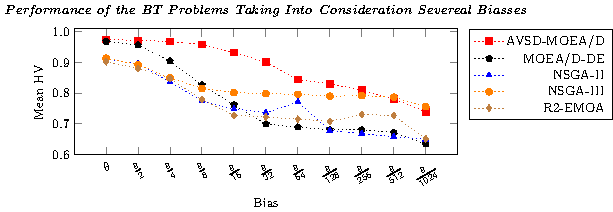
\includegraphics[width=0.85\textwidth]{images/BIAS_Full-figure0.eps} \\
\caption{Mean of \HV{} values for eight \BTS{} problems (y-axis) against several biasses ratios (x-axis). The \BT{}2 problem is not taken into consideration due that it suffers of numerical stability.}\label{fig:BT}
\end{figure}

\section{On the Convergence of \MOEAS{} in Test Problems with Bias Features}

As pointed out in~\cite{li2016biased, deb1999multi, huband2006review}, the bias feature is one of the most challenging difficulties that \MOEAS{} might face.
%
Recently, the \BTS{} test problems were proposed to facilitate the study of the ability of \MOEAS{} for dealing with biases.
%
In this context bias means that small variations in the decision space around the Pareto set cause significant changes in vicinities of some Pareto front solutions~\cite{huband2006review}.
%
Particularly, those problems are built with transformations that induce position-related bias and distance-related bias.
%
While the former means that a small change on the position-related variables of one solution in the Pareto set projects a significant change along the Pareto front.
%
The later imposes that a small variation on the distance-related variables of one solution in the Pareto set causes a significant deterioration on the convergence towards the Pareto front.
%

In order, to analyze the capability of the \MOEAS{} to deal with bias features the \BTS{} problems are taken into account.
%
Specifically, this section analyses the sensitivity of the algorithms imposing several levels of bias in the distance-related variables.
%
Initially, for each problem the position-related bias and distance-related bias ($\theta$) are kept exactly as the one proposed in the original work~\cite{li2016biased}.
%
Then, for each problem its initial distance-related bias value ($\theta$) is iterativelly decreased by a factor of two.
%
Specifically, the distance-related bias taken into account are $\{\theta, \frac{\theta}{2}, \frac{\theta}{4}, \frac{\theta}{8}, \frac{\theta}{16}, \frac{\theta}{32}, \frac{\theta}{64}, \frac{\theta}{128}, \frac{\theta}{256}, \frac{\theta}{512}, \frac{\theta}{1028}\}$.
%
Figure~\ref{fig:BT} shows the mean \HV{} ratio obtained with several distance-related biasses. 
%
Also note that the \BT{}2 problem is not taken into consideration due that increasing its bias values provokes numerical instability since that it incorporates a different bias transformation, nevertheless all the results can be consulted in the supplementary document.
%
Taking exactly the original configuration (bias of $\theta$)~\cite{li2016biased} \AVSDMOEAD{} is sigthly better than \MOEADDE{}, but as soon as the bias is decreased to $\frac{\theta}{32}$ the performance of \MOEADDE{} decays aggressively.
%
Furthermore, the performance of \AVSDMOEAD{} is superior than $0.9$ with biasses values upper or equal to $\frac{\theta}{256}$ which is quite superior than the state-of-the-art \MOEAS{} whose values at that point are approximately of $0.75$.
%
Figure~\ref{fig:attainment_BT} shows the 50\% of attainment surface of \BT{}6, \BT{}7 and \BT{}8 with a bias of $\frac{\theta}{32}$.
%
\BT{}6 and \BT{}8 have simple nolinear Pareto set while \BT{}7 has a complicated nolinear Pareto set.
%
\BT8{} is multimodal.
%
Although that \MOEADDE{} converged to a region of the Pareto front with \BT{}6 \AVSDMOEAD{} covered a huge region of the Pareto front, in fact this shows that for this problem promoting diversity in the decision space results in diversity in the objective space.
%
In addition, \AVSDMOEAD{} converges quite well in complicates nonlinear Pareto sets shown in the 50\% attained surface of \BT{}7 (Figure~\ref{fig:attainment_BT}).
%
Finally but not less important \AVSDMOEAD{} shows a superior behaviour with biased and multimodal problems as is the case of \BT{}8 whose attainment surfaces have converged much better to the Pareto front.




%% The Appendices part is started with the command \appendix;
%% appendix sections are then done as normal sections
%% \appendix

%% \section{}
%% \label{}

%% References
%%
%% Following citation commands can be used in the body text:
%% Usage of \cite is as follows:
%%   \cite{key}          ==>>  [#]
%%   \cite[chap. 2]{key} ==>>  [#, chap. 2]
%%   \citet{key}         ==>>  Author [#]

%% References with bibTeX database:

% \bibliographystyle{model1-num-names}

%% New version of the num-names style
\bibliographystyle{elsarticle-num-names}
\bibliography{bibtex/References.bib}

%% Authors are advised to submit their bibtex database files. They are
%% requested to list a bibtex style file in the manuscript if they do
%% not want to use model1-num-names.bst.

%% References without bibTeX database:

% \begin{thebibliography}{00}

%% \bibitem must have the following form:
%%   \bibitem{key}...
%%

% \bibitem{}

% \end{thebibliography}


\end{document}

%%
%% End of file `elsarticle-template-1-num.tex'.
